% region preamble
\documentclass[11pt]{article}
\usepackage{import}
\usepackage[margin=1in, top=1in]{geometry}
\usepackage[all]{nowidow}
\usepackage[hyperfigures=true, hidelinks, pdfhighlight=/N]{hyperref}
\usepackage[separate-uncertainty=true, group-digits=false]{siunitx}
\usepackage{graphicx,amsmath,physics,tabto,float,amssymb,pgfplots,verbatim,tcolorbox}
\usepackage{listings,xcolor,subcaption,caption,import,wrapfig,lipsum,tikz,dirtree}
\usepackage{minted,soul}
\usepackage[sorting=none]{biblatex}
\usepackage[version=4]{mhchem}
\usepackage[noabbrev]{cleveref}
\newcommand{\creflastconjunction}{, and\nobreakspace}
\newcommand{\mb}[1]{\mathbf{#1}}
\newcommand{\pt}{p_\mathrm{T}}
\newcommand{\Cppinline}[1]{\mintinline{c++}{#1}}
\numberwithin{equation}{section}
\numberwithin{figure}{section}
\numberwithin{table}{section}
\definecolor{stringcolor}{HTML}{C792EA}
\definecolor{codeblue}{HTML}{2162DB}
\definecolor{commentcolor}{HTML}{4A6E46}
\definecolor{LightGray}{HTML}{eaeaea}
\captionsetup{font=small, belowskip=0pt}
\usemintedstyle{vs}
\setminted{framesep=2mm,bgcolor=LightGray,fontsize=\footnotesize,linenos,breaklines}
\let\OldTexttt\texttt
\sethlcolor{LightGray}
\renewcommand{\texttt}[1]{\OldTexttt{\hl{#1}}}
\renewcommand{\lstlistingname}{Appendix}
\pgfplotsset{compat=1.17}
\addbibresource{bibliography.bib}
% endregion

\title{{\Huge A preliminary analysis of data from ALICE's new ITS and MFT detectors}}
\author{{\Large Miles Kidson}\\ \\
Supervisors: Prof. Zinhle Buthelezi, Dr. SV Fortsch, \& Prof. Tom Dietel\\
Assisted By: Dr. B Naik (Postdoctoral fellow)}
\date{\textbf{UCT Honours 2022}}

\begin{document}
\pagenumbering{roman}
\maketitle

\begin{figure}[h]
    \begin{center}
        
\includegraphics{Figs/UCT.jpg}
    \end{center}
\end{figure}

\begin{abstract}
    \centering
    We investigate pilot-beam data from proton-proton collisions in Run 3 at ALICE, tracing its journey through two of the new detectors (the Inner Tracking System and Muon Forward Tracker) and the new Online-Offline analysis framework. The data is analysed to assess the performance of the detectors with the expectation of isotropic emission of particles, taking their geometry into account. Recommendations for improvements to the analysis framework and documentation are given.
\end{abstract}

\newpage
\tableofcontents

\newpage
\listoffigures

\newpage
\pagenumbering{arabic}
\setcounter{page}{1}
\section{Introduction}\label{sec:Introduction}
The ALICE (A Large Ion Collider Experiment) detector is a detector experiment at the Large Hadron Collider (LHC) at CERN. Its primary goal is the investigation of ``strongly interacting matter at extreme energy densities, where a formation of a new phase of matter, the quark-gluon plasma, is expected''~\cite{ALICE_LOI}. It achieves this goal by studying the products of head-on collisions of heavy ions such as lead, called Pb-Pb collisions for short. It also studies proton-lead (p-Pb) and proton-proton (p-p) collisions. 

Run 3 is the latest period of data capture at the LHC, with an intended centre of mass energy per collision of $\sqrt{s}=\SI{13.6}{\tera\electronvolt}$ and increased luminosity of collisions---a factor 10 increase in integrated luminosity for Pb-Pb collisions. For Run 3, ALICE is moving from a triggered read-out system to a combination of triggered and continuous read-out. In order to achieve this, many detectors and their front-end electronics were upgraded, some new detectors were added, and the analysis framework was overhauled entirely. 

Of the upgrades to ALICE, the following are the subject of this report. The Inner Tracking System (ITS) was upgraded with an entirely new pixel detector technology, hoping to greatly increase the resolution when determining the primary collision vertex. The Muon Forward Tracker (MFT) is one of the new detectors added. Its primary use is to assist the Muon Spectrometer (MCH) with vertexing and tracking in the forward region of ALICE and uses the same technology as the ITS. To deal with the increased volumes of data, a new analysis framework was introduced called Online-Offline (O2). 

This report aims to introduce the detectors and the data they output, trace the path of that data through the new analysis framework until it arrives at our desk, and show the details of the analysis we performed to determine if the upgrades are working as expected. The data used in this report is from two proton-proton collision runs performed in October 2021, at a centre-of-mass energy of \SI{900}{\giga\electronvolt}. This is not an energy we expect to use for physics data analysis but is good enough for this purpose.

\section{Background \& Detector Theory}\label{sec:Background_Detector}
\subsection{Coordinates}
The coordinate system used at ALICE needs to be discussed in order to fully explain the scope of this report. A modified cylindrical coordinate system, shown in \cref{fig:coords}, is used as most detectors in the experiment are cylindrically symmetric about the beamline of the LHC. 

\begin{figure}[h]
    \begin{center}
        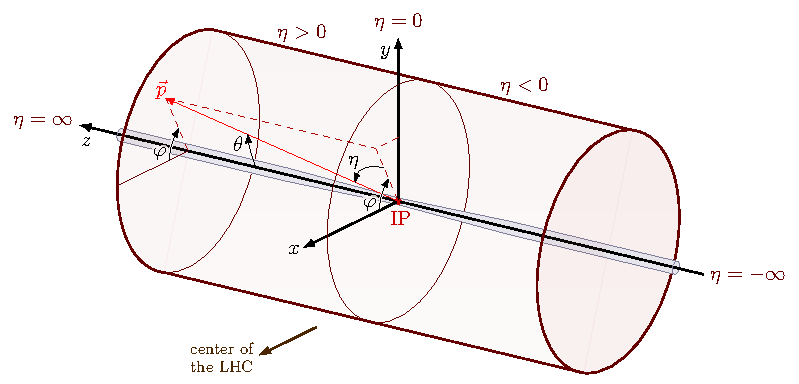
\includegraphics[width=.8\textwidth]{Figs/coords.pdf}
        \caption{Modified cylindrical coordinate system used at the LHC~\cite{coords}.}
        \label{fig:coords}
    \end{center}
\end{figure}

We place the $z$-axis along the beamline with its origin at the interaction point (IP). The IP is the point at which collisions happen, right in the center of the detector. The angle around the $z$-axis is called the azimuthal angle, denoted by $\varphi$. Sometimes in the literature $\varphi$ ranges from 0 to $2\pi$ and sometimes it ranges from $-\pi$ to $\pi$. We will try stay consistent and use the latter in this report, but we may need use the other convention at times. The angle from the $z$-axis to the $x$-$y$ plane is called the polar angle, denoted by $\theta$, and runs from 0 to $\pi$. We are interested in the standard 3-momentum of particles that we track in the detector, which we call $\vec{p}=(p_x,p_y,p_z)$, but we also define the transverse momentum as 
\begin{equation}
    p_{\mathrm{T}}=\sqrt{p_x^2 + p_y^2}.
    \label{eqn:transverse momentum}
\end{equation}
We define the rapidity, often denoted as $y$, as
\begin{equation}
    y=\frac 12 \ln\left(\frac{E+p_z}{E-p_z}\right)
    \label{eqn:rapidity}
\end{equation}
where $E$ is the total energy of the particle being considered and $p_z$ is the momentum in the $z$ direction~\cite{kar_exp_phys}. This quantity is useful as differences in rapidity are Lorentz invariant for boosts along the $z$-axis. One issue, however, is that the energy of a particle is hard to measure, so we instead use pseudorapidity, denoted as $\eta$. Rapidity and pseudorapidity are equivalent for massless particles, and near equivalent for particles with total 3-momentum magnitude $p$ much greater than their mass $m$. Pseudorapidity is much easier to measure as it is defined in \cite{kar_exp_phys} as
\begin{equation}
    \eta=-\ln\tan\frac{\theta}{2}.
    \label{eqn:pseudorapidity}
\end{equation}
From \cref{fig:coords} we see that for $z$ positive, $\eta$ is also positive, and similarly for $z$ negative. Confusingly, we define the ``forward region'' of the ALICE detector as the region for which $z$, and thus $\eta$, are negative. The forward region is where our interest lies.

The four coordinates that we use most often are $z$, $\varphi$, $p_\mathrm{T}$, and $\eta$. 

\subsection{ALICE Run 3}
In 2018, the LHC shut down for what was called Long Shutdown 2 (LS2). During this time, the ALICE experiment was being prepared for Run 3, where it will be taking data at higher energies and much higher luminosities than before, from 2022 until 2025~\cite{ALICE_Upgrade_LOI}. \Cref{fig:ALICE_Schematic} shows the detector configuration for Run 3. The intent of these upgrades was in large part to prepare ALICE for a higher luminosity of collisions in both Pb-Pb and p-p cases. 

Part of the upgrades for Run 3, the details of which can be found in \cite{ALICE_Upgrade_LOI}, were a whole new Inner Tracking System and a brand new detector called the Muon Forward Tracker. These detectors are both silicon-based and their primary purpose is tracking particles and determining the collision vertex, which is the best estimation of where the collision that resulted in these particles happened. 

The readout electronics for many detectors were upgraded to allow for continuous readout where necessary. The MCH also had its readout and front-end electronics upgraded but will still work on a triggered readout system.

\begin{figure}[h]
    \begin{center}
        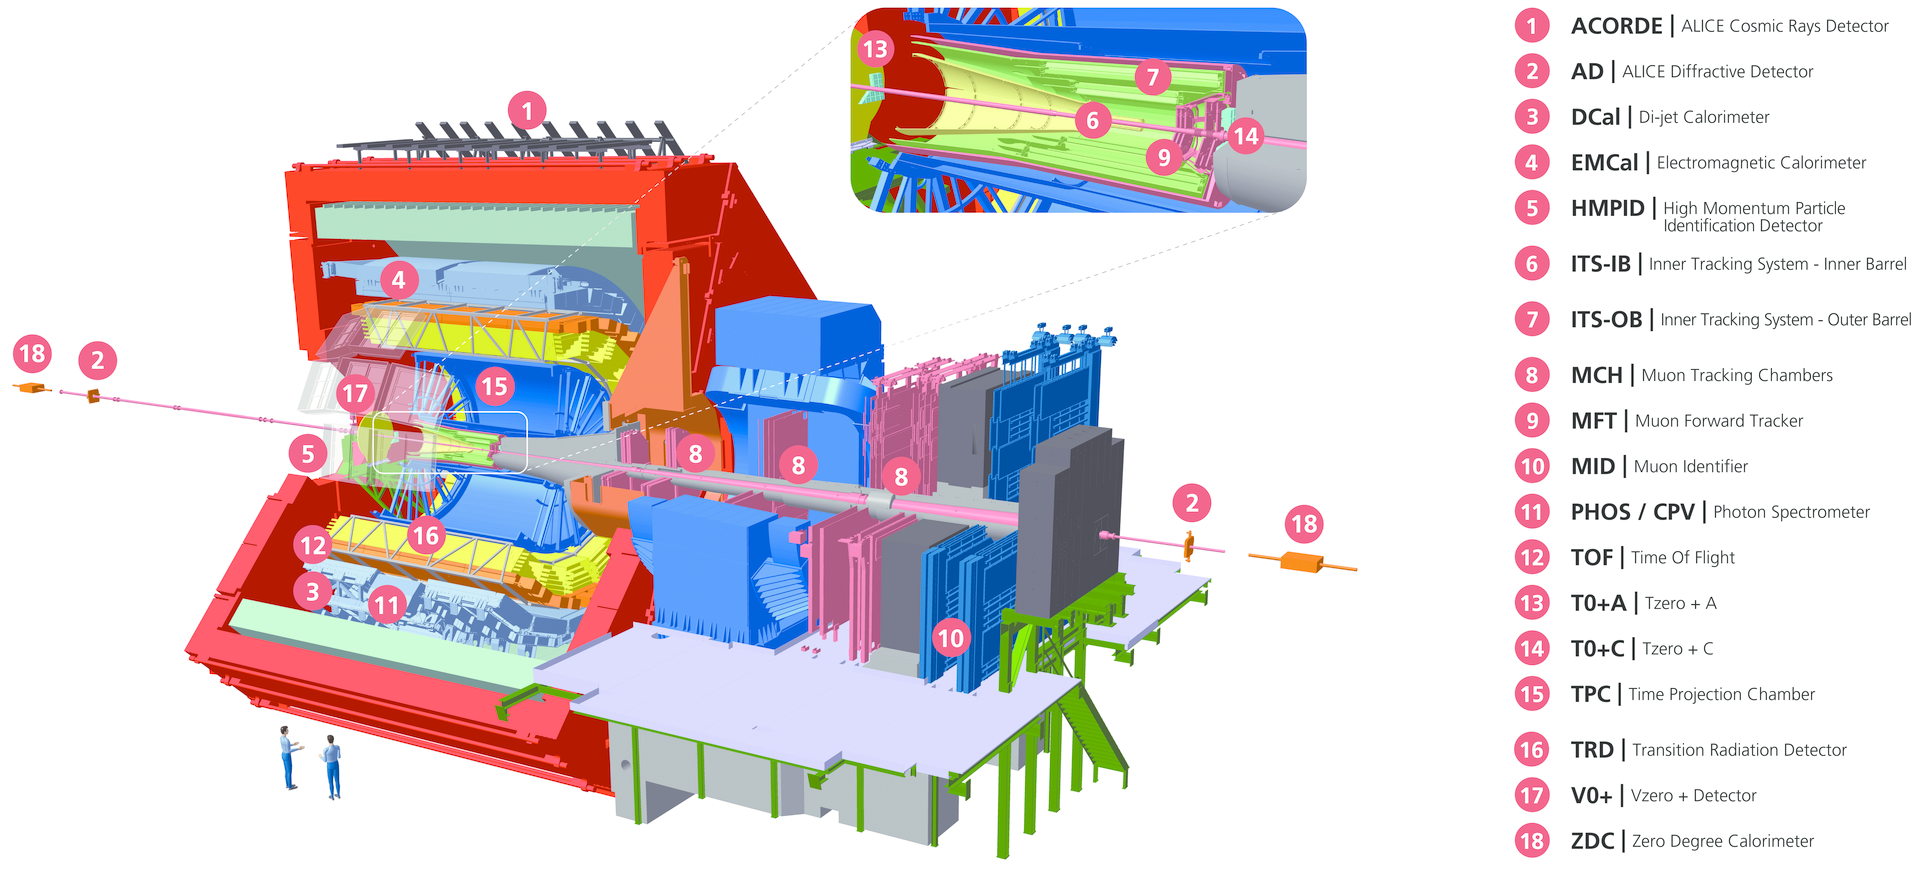
\includegraphics[width=\textwidth]{Figs/ALICE_RUN3_schematic.png}
        \caption{Schematic view of the ALICE detector setup for Run 3 of the LHC~\cite{ALICE_schematic_labels}. Note here that the MCH is shown separate from the MID, which act as the triggering mechanism for the MCH. For the purposes of this report, the MID will be considered part of the MCH. The ITS (6, 7), MCH (8), and MFT (9) are the focus of this report.}
        \label{fig:ALICE_Schematic}
    \end{center}
\end{figure}


\subsection{The Inner Tracking System}
The Inner Tracking System (ITS) sits in the main barrel of ALICE, as seen in \cref{fig:ALICE_Schematic}, and covers the range $|\eta|<1.22$~\cite{ITS_Upgrade_TDR}. For Run 3 it has been upgraded significantly by replacing the old detector with a new layout and new pixel detector technology, leading to an improvement in track position resolution at the primary vertex of a factor of 3 or greater~\cite{ITS_Upgrade_TDR}. The ITS's main purpose is to track the particles resulting from the collisions and determine the position of the primary vertex of collisions. It also serves to ``reconstruct secondary vertices, track and identify particles with low momentum, and improve the momentum and angle resolution for particles reconstructed by the Time Projection Chamber (TPC)''~\cite{ITS_Info}.

\begin{figure}[h]
    \begin{center}
        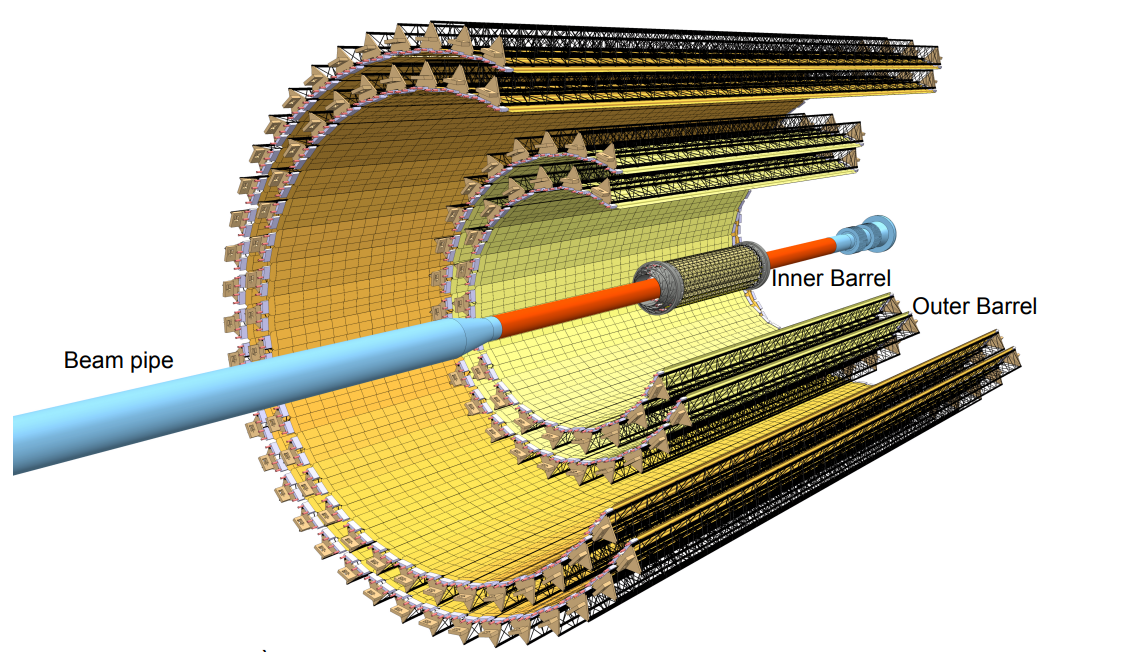
\includegraphics[width=.8\textwidth]{Figs/ITS_Schematic.png}
        \caption{Schematic view of the Inner Tracking System~\cite{ITS_Upgrade_TDR}. Note the thinner beam pipe and extremely close Inner Barrel.}
        \label{fig:ITS_Schematic}
    \end{center}
\end{figure}

The new ITS consists of 7 layers of pixel detectors; 3 in the ``Inner Barrel'' and 4 in the ``Outer Barrel''. The innermost layer sits at a radius of only \SI{22.4}{\milli\metre} from the IP thanks to a reduction in beam pipe radius for Run 3 and the outermost layer sits at a radius of \SI{391.8}{\milli\metre} from the IP. \Cref{fig:ITS_Schematic} shows the layout more clearly. 

The pixel detectors used are \SI{0.18}{\micro\metre} CMOS chips from TowerJazz. When a charged particle passes through the silicon in the active volume, it liberates the charge carriers in the material, which then collect on electrodes connected to the silicon, telling the detector that a particle has been detected. The fine segmentation of the detectors also allows the detector to determine the point at which the particle hit the detector, up to a resolution of \SI{4}{\micro\metre} in both the $r\varphi$ and $z$ directions~\cite{ITS_Upgrade_TDR}. The amount of charge deposited on the detector is dependent on the particle species and momentum (Bethe-Bloch). 

Two main methods of readout were considered for the ITS in the new continuous readout scheme. Firstly, a rolling shutter which continually loops through the rows of pixels and reads out the charge deposited on that pixel in the time since the last readout was considered. The time between readings, known as the integration time, for the first method is around \SI{30}{\micro\second}. The rolling shutter scheme lends itself to needing a small number of transistors within each pixel. The second scheme is known as ALPIDE, where each pixel has a comparator that signals when the pixel has an analogue signal greater than the comparator's threshold. The signalled pixels then get read out asynchronously, according to their priority in the chain. This scheme has an effective integration time of around \SI{4}{\micro\second} but has a larger material budget. 

\textbf{\textit{FIND OUT WHICH ONE WAS USED SMH}}




\subsection{The Muon Spectrometer}
The MCH sits in the forward region of ALICE, as seen in \cref{fig:ALICE_Schematic}, and covers $-4<\eta<-2.5$. It is designed to study heavy quark resonances through their single- and di-muon decay channels. As is shown in \cref{fig:Muon Spectrometer}, it is composed of a hadronic absorber, 5 tracking chambers, a dipole magnet, another absorber, and finally the 2 trigger chambers. The MFT is often also considered part of the MCH but is not shown in \cref{fig:Muon Spectrometer}. The section is adapted from the MCH Technical Design Report~\cite{MCH_TDR}.

\begin{figure}[ht]
    \begin{center}
        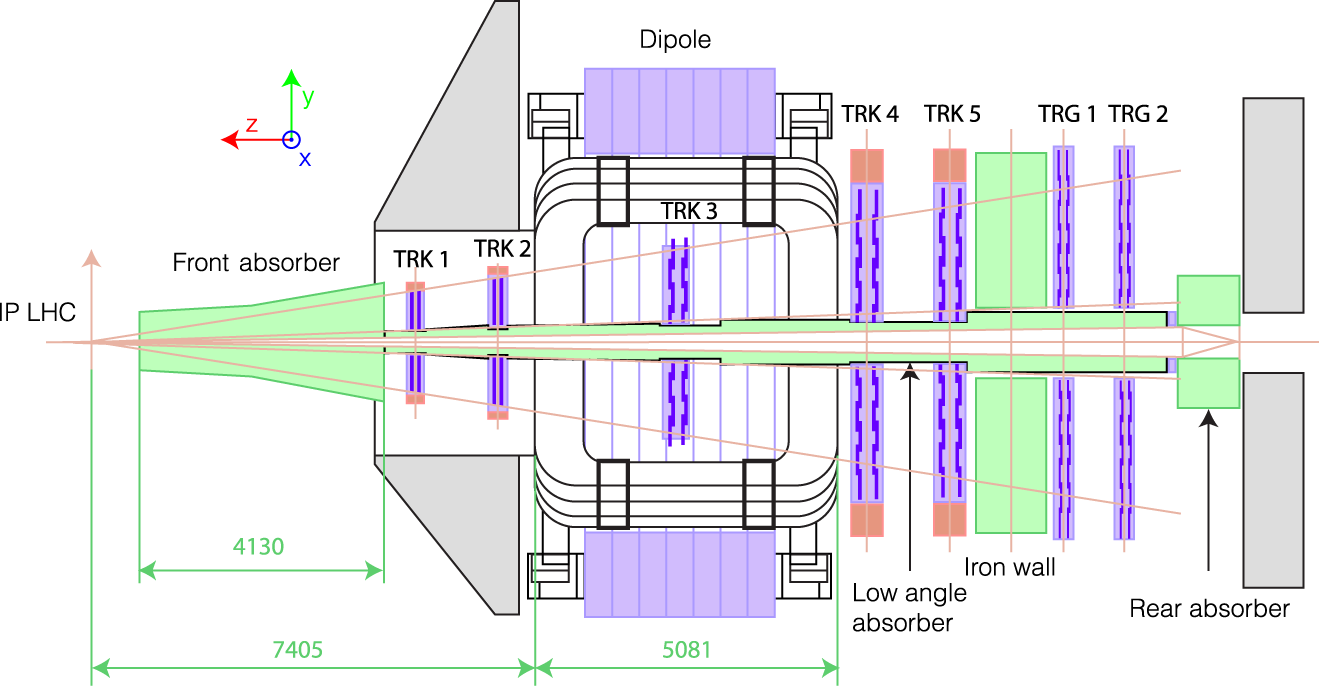
\includegraphics[width=0.8\textwidth]{Figs/MCH_schematic_pog.png}
        \caption{Diagram of the layout of the Muon Spectrometer~\cite{Muon_Spec_Schematic}. Muons pass through the absorber, are deflected by the dipole magnet, and hit the trigger chambers at the back. Importantly, all detector material sits behind the hadronic absorber, meaning the amount of data that can be used for tracking and vertexing is much lower than, say, the ITS.}
        \label{fig:Muon Spectrometer}
    \end{center}
\end{figure}

Muons don't tend to interact with matter much, especially when compared to hadrons and electrons. This makes studying muons easier, to some degree, since most other particles can be filtered out by making them pass through a large chunk of matter. As is shown in \cref{fig:Muon Spectrometer}, that is exactly what is done in the MCH. In front of any detector material (ignoring the MFT for now) sits the hadronic absorber, made primarily of carbon and concrete. This is intended to filter out all non-muon particles (mainly hadrons and photons) while not reducing the muon energy much so that they can still be studied. 

After the absorber are 5 sets of 2 cathode pad tracking detectors, situated around a large warm dipole magnet. Particles that make it through the absorber get picked up by the first two sets of detectors, then pass through the magnetic field and are deflected according to their charge, mass, and momentum. The third set tracks the particles during deflection and then the last two detect them after deflection. This set-up is particularly useful for studying di-muon events as the muons produced would be a muon-antimuon pair, which would deflect in opposite directions in the dipole magnet. This would leave a characteristic track signature that can be studied.

After the last tracking detector, particles pass through another absorber, which serves to further filter out muons from background, as well as filter out background muons. The muons produced in heavy quark resonances have considerably higher $\pt$ than those produced by background processes, so the job of the trigger system is to only trigger on muons with high enough $\pt$ to be interesting (this is defined per process) and the second absorber helps reduce the number of background muons incident on the trigger system. The trigger system is made of 2 stations of 2 Resistive Plate Chamber (RPC) detectors. Comparing the measurement of the same particle in the two stations, the $\pt$ can be determined. The decision to keep or reject an event takes about \SI{300}{\nano\second}.

In Run 1 and Run 2, the MCH performed all its own tracking and vertexing on the particles it studied. Particularly for vertexing, where the collision position is estimated, this was not optimal as most of the particles produced in the interactions didn't make it through to sensitive material. With the increased energy and luminosity of Run 3 a better system was needed to perform these tasks, so the MFT was added in front of the first absorber to take over the job.


\subsection{The Muon Forward Tracker}
The MFT is a brand new detector added to ALICE for Run 3 to assist the MCH with tracking and vertexing. It covers the range $-3.6<\eta<-2.45$ and was designed in conjunction with the ITS, using precisely the same CMOS pixel detectors. Due to the MFT being placed in front of the absorber, it detects a lot more particles than make it through to the MCH, allowing it to be much better at finding the primary vertex of collisions. \Cref{fig:MFT Schematic} shows the design of the MFT. The rest of this section is adapted from the MFT Technical Design Report~\cite{MFT_TDR}. 

\begin{figure}[h]
    \begin{center}
        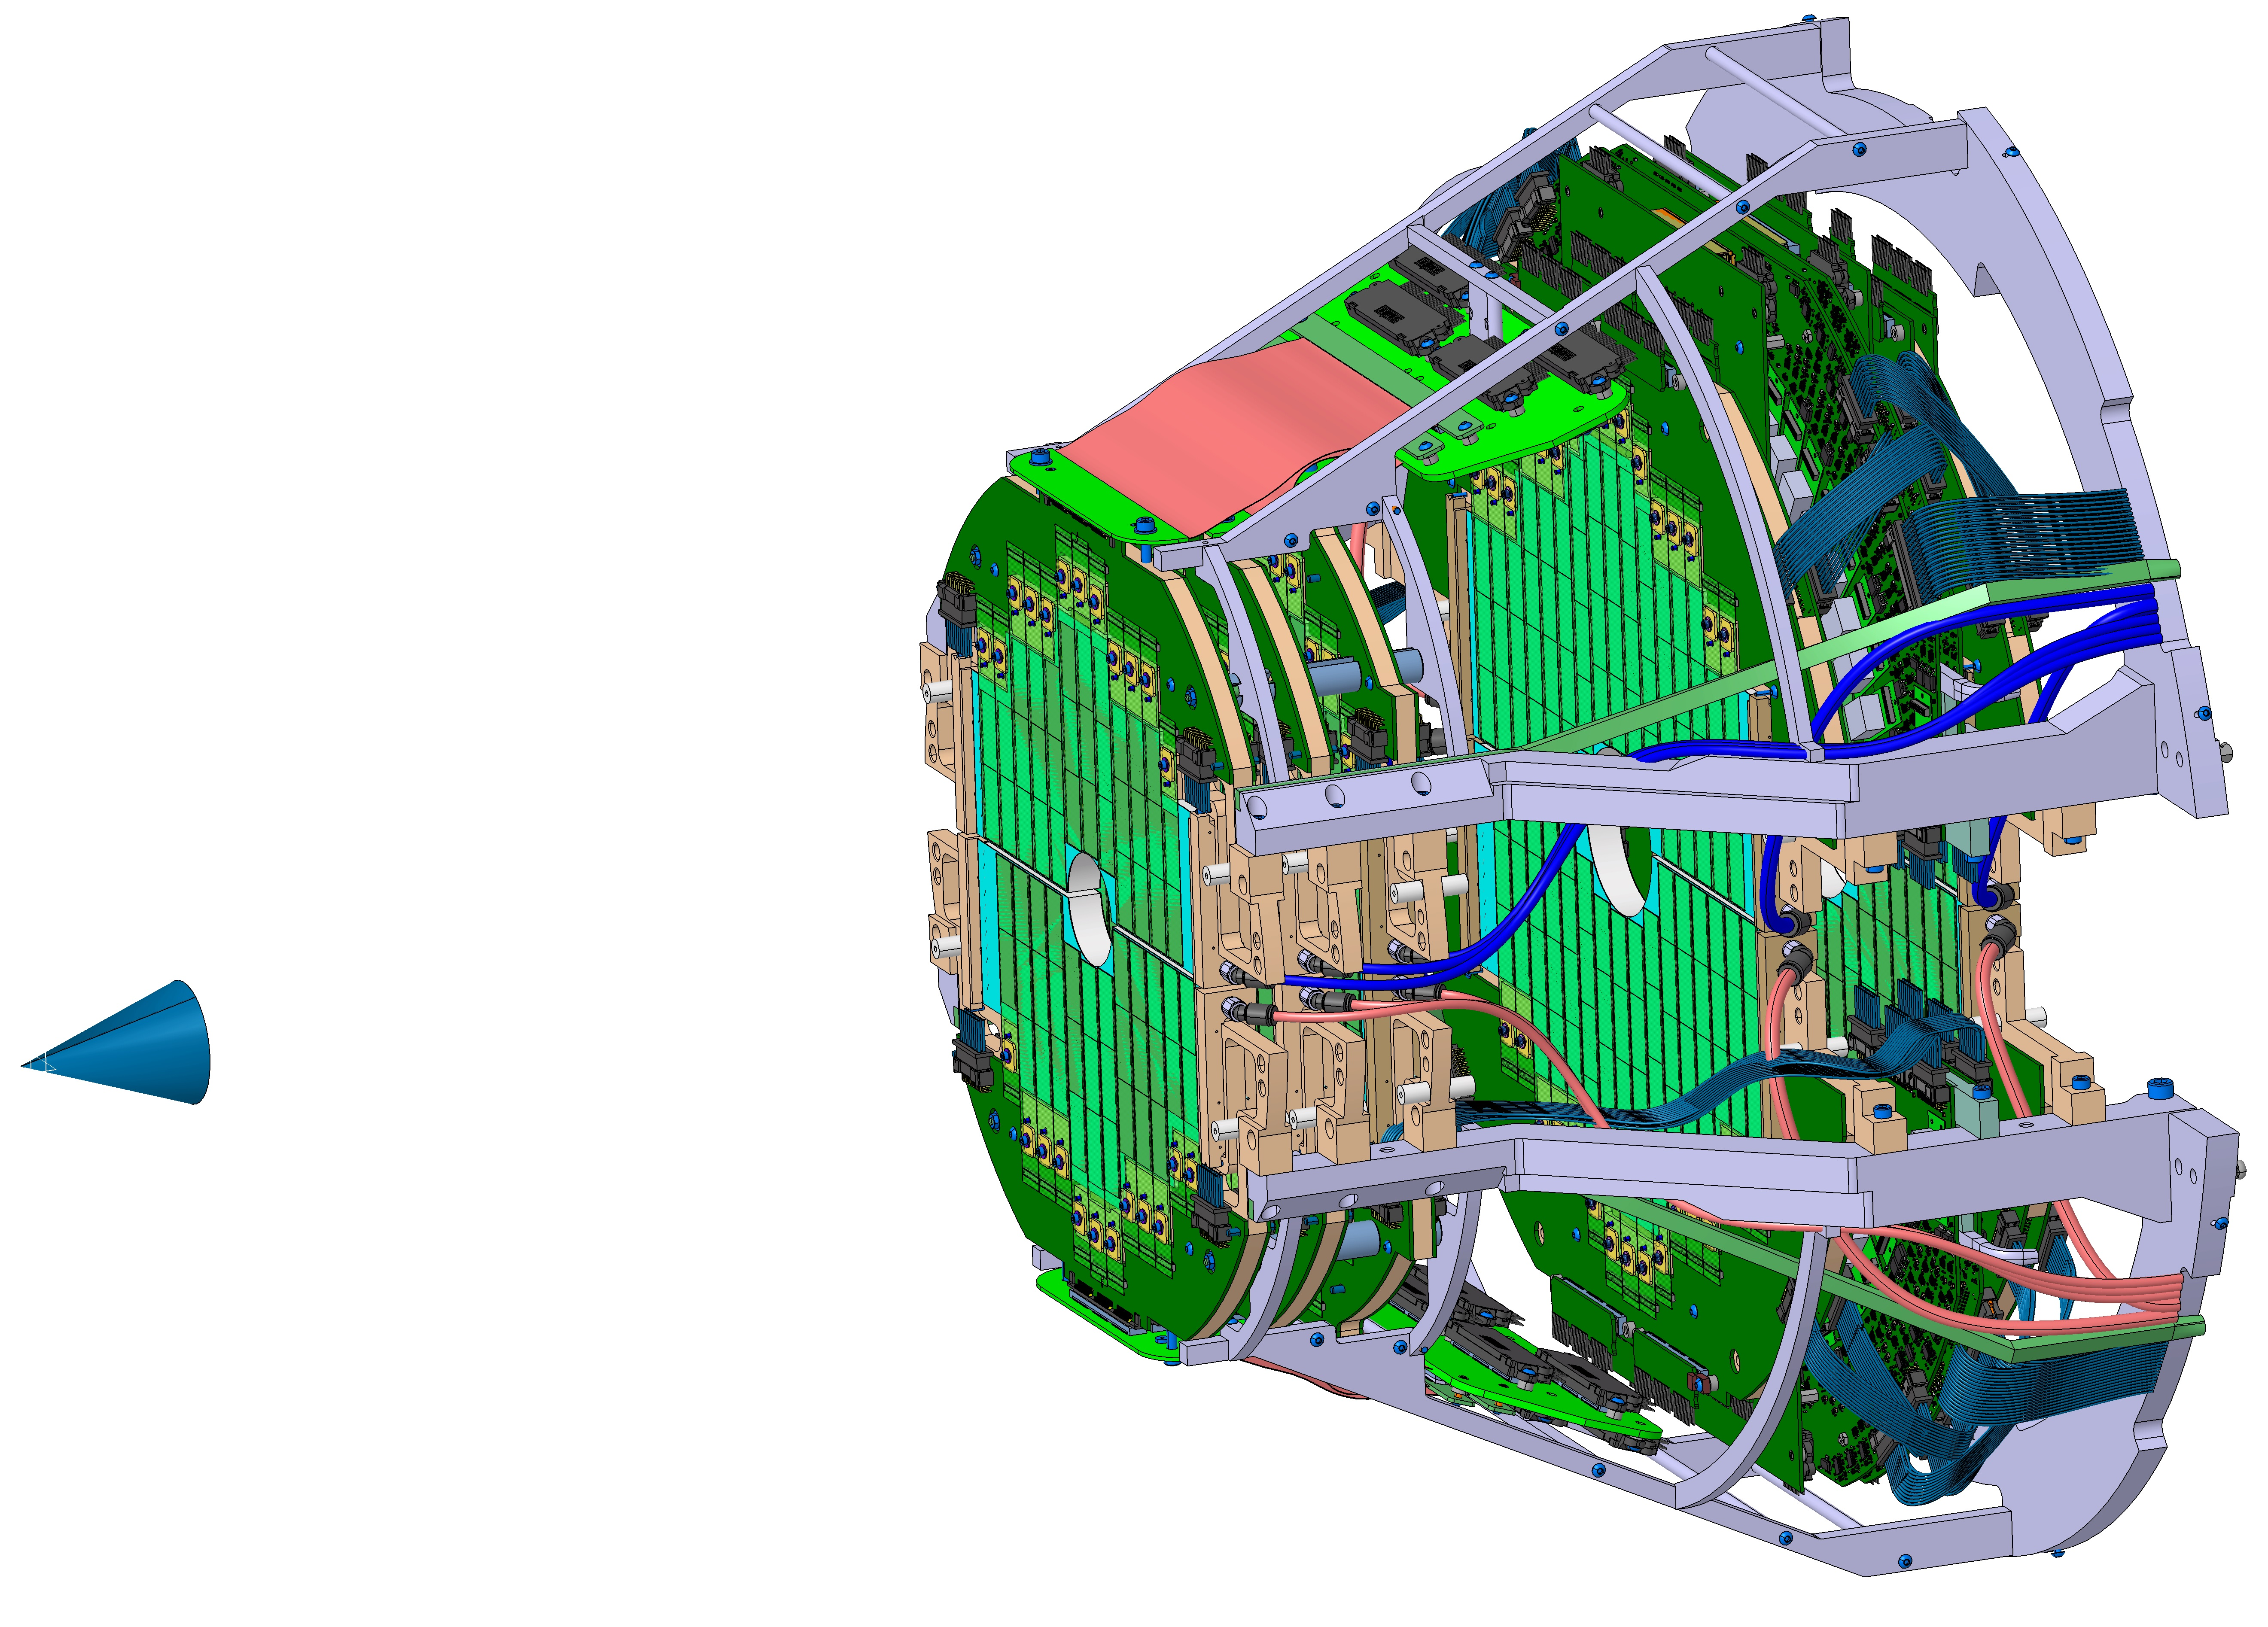
\includegraphics[width=.8\textwidth]{Figs/MFT_schematic.jpg}
        \caption{Schematic view of the Muon Forward Tracker~\cite{MFT_Schematic}. The small cone on the left shows the IP. Note that the 5 disks each have a front and back plane of pixel detectors, totalling 10 $z$-positions for the MFT to ``see'' particles at.}
        \label{fig:MFT Schematic}
    \end{center}
\end{figure}

The MFT is made of two identical half-cones sandwiching the beam pipe from above and below, each with 5 half-disks positioned at different distances from the IP along the $z$-axis. Each half-disk has a front and back detection plane totalling 10 detection planes. As the disks get further from the IP their radius increases in order to cover the same $\eta$ range, aside from the second disk, which is identical to the first. The disks sit at $z$-positions -46.0, -49.3, -53.1, -68.7, and -76.8 \si{\centi\metre} respectively and each disk is \SI{1.4}{\centi\metre} thick, leading to detector planes at $\pm \SI{0.7}{\centi\metre}$ from each of those positions.

\begin{figure}[h]
    \begin{center}
        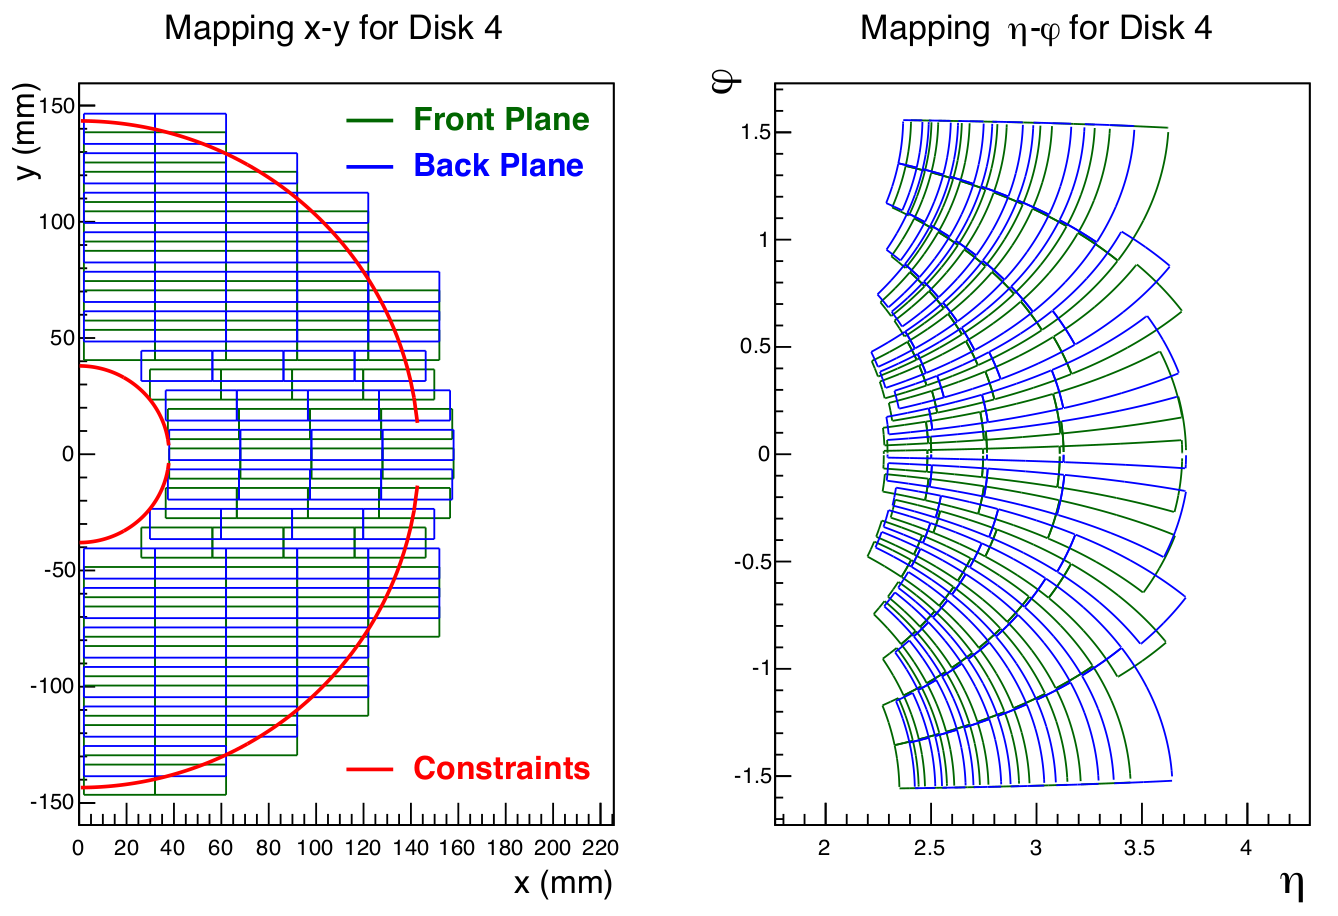
\includegraphics[width=.8\textwidth]{Figs/MFT_Disk4_mapping.png}
        \caption{The layout of pixel detector elements on the front and back plane of one of the half-disks of disk 4 in the MFT. Note that the front and back plane have layouts offset to each other by half the width of the pixel elements. \textbf{\textit{SOMETHING WEIRD ABOUT THIS PLOT. I THINK X AND Y ARE WRONG}} \cite[fig.~6.1]{MFT_TDR}}
        \label{fig:MFT_Disk4_mapping}
    \end{center}
\end{figure}

The half-disks are made from ladders of 2 to 5 rectangular pixel detector elements. \Cref{fig:MFT_Disk4_mapping} shows an example of the layout of the front and back planes of detector elements in both $x$-$y$ and $\eta$-$\varphi$. 




\subsection{The Online-Offline Analysis Framework}
With the increased interaction rate expected for Run 3, a new system for real-time processing, as well as offline analysis, needed to be constructed \cite{ALICE_Upgrade_LOI}. The Online-Offline (O2) framework was developed for this purpose. The ``Online'' portion of the framework is the real-time processing, where continuously captured data from ALICE is split into \SI{10}{\milli\second} chunks, called timeframes. These timeframes are then later processed, or ``reconstructed'' into Event Summary Data (ESD) and then Analysis Object Data (AOD) files---this is the ``Offline'' part---which contain only the data of interest. Different passes of reconstruction can be done for purposes and are often iterated upon if something was missed in a previous pass. Because of this, the same data can often look different between reconstruction passes. The AOD files can then be analysed---also Offline---through an ``Analysis Task'', written in C\OldTexttt{++} and ROOT. 

We distinguish between data taken in Run 3 and data taken in Run 1 and 2 by calling Run 3 AOD's ``AO2D'' files, and Run 1 and 2 just ``AOD'' files. The data is stored on the \OldTexttt{alimonitor} system, requiring a certificate to access, which is obtained by joining the ALICE collaboration. Access to all data and most analysis tools used in this report is restricted behind this wall. 

\begin{figure}[h]
    \begin{center}
        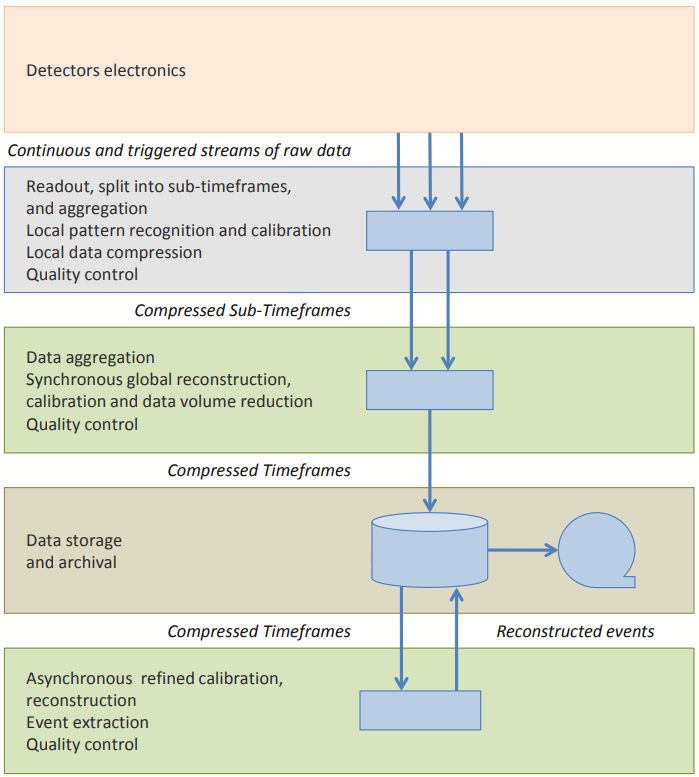
\includegraphics[width=.6\textwidth]{Figs/O2_flow.png}
        \caption{Functional flow of the O2 framework~\cite{O2_Upgrade_TDR}. Detectors output their signal continuously in the new configuration and this signal gets split into chunks called timeframes. These timeframes get processed a number of times, reducing the volume of data each time by only extracting the quantities that will be used for analysis. Many choices have to be made at each step to ensure that useful data makes it out the other side and so the details of this process are always in flux.}
        \label{fig:O2_flow}
    \end{center}
\end{figure}

The focus of the upgraded analysis framework was to reduce disk space usage when processing and analysing, as well as making sure all analysis takes advantage of all processing power available to it at all times. \Cref{fig:O2_flow} shows the general flow of data in the O2 processing pipeline from particle hits in detectors until usable data in the form of AOD files. 



\section{Analysing Using O2}\label{sec:AnalysingWithO2}
One of the main goals of O2 is to take away as much responsibility from the user as possible when it comes to managing memory, writing efficient code, and disk space usage. To this end, writing an analysis task in O2 is structured quite strictly. This section will outline the information needed when trying to analyse reconstructed data to produce, in our case, histograms of kinematic variables. 

It must be noted that learning how to do this, and how to deal with the idiosyncrasies of the O2 software, is what took up the majority of the time spent on this project. O2 is written to do one thing very, very well, but unfortunately that comes with the side-effect of it being extremely picky about the conditions in which the software will actually work. Lastly, a distinction needs to be made between O2 and O2Physics. O2 generally refers to the entire analysis framework, including both the online and offline parts. This encompasses O2Physics, which is used only for offline analysis. Despite this, in terms of the structure of the software, O2 and O2Physics are separate things but O2Physics sometimes depends on O2. For this reason it can become ambiguous when discussing O2 and O2Physics but we will try our best to keep them distinct. 

\subsection{AOD Structure}\label{sec:AODStructure}
The data that we use in our analysis comes in the form of Analysis Object Data. These get produced asynchronously and come in the form of ROOT files containing ``Dataframes''. These are organised in a tree structure where each tree contains a number of tables, for example a table containing collisions and a table containing tracks. The tables have columns which hold variables corresponding to each entry, or row, in the table. There are 4 types of column:

\begin{itemize}
    \item Static columns are saved to disk during the reconstruction process and are available at any time. The $z$-position of a collision vertex, for example, is a static variable.
    \item Dynamic columns are defined as functions with inputs from static variables (or variables input by the user). They will produce a result on demand in order to save memory and disk space. Momentum in the $x$-direction is a dynamic variable.
    \item Index columns point from one table to another, such as from a track to its associated collision. They can also refer to their own table, such as for an MC particle to refer to its mother or daughter particle after decay.
    \item Expression columns are similar to dynamic columns in that they get calculated on demand, but they get evaluated on all entries in a table upon requesting it and produce a column that can then be accessed as if it were a static column. Importantly, dynamic columns cannot be used as inputs to expression columns.
\end{itemize}

\subsection{Analysis Task Structure}\label{sec:TaskStructure}
Analysis tasks are written in C\OldTexttt{++} and need to be structured in a specific way so that O2Physics to use them properly. Each task is written as a \texttt{struct} object which is then called at the end of the task. Below is an outline of what is needed for a task.

\begin{minted}{c++}
#include "Framework/runDataProcessing.h"
#include "Framework/AnalysisTask.h"

using namespace o2;

struct MyTask {
  // Define things here, such as histogram registries, filters for data, or new tables

  void init(o2::framework::InitContext&) {
    // Here we initialise histograms and other things used in the analysis
  };
  // The arguments of the process function are where we subscribe to specific tables in the AOD that we're analysing. 
  void process(aod::Collision const& collision, aod::Tracks const& tracks) {
    // Here we can do any processing that we need, calculating things etc, and then fill the histograms we defined earlier
  };
};

// This is what O2 looks at to run the task
WorkflowSpec defineDataProcessing(ConfigContext const& cfgc)
{
  return WorkflowSpec{
    adaptAnalysisTask<MyTask>(cfgc),
  };
}
\end{minted}

\subsection{Table Features}
All variables associated with a track, for example, could be included in a single table. However, since we often only need a few of the variables, the tables are split up into sections that contain variables often used together. If needed, these tables can be joined together when doing analysis using \texttt{o2::soa::Join<Table1, Table2>}. Importantly, only tables which correspond row-to-row and have the same number of rows can be joined in this way.

We might also want to only access entries in a table that pass some filter, say having $|\eta| < 0.8$. We can do this by putting \texttt{Filter f = nabs(aod::track::eta) < 0.8;} somewhere before the \texttt{process} function and then instead of subscribing to \texttt{aod::Tracks} as we have done, we can put \texttt{soa::Filtered<aod::Tracks> const\& filteredTracks} in the \texttt{process} function call. Multiple filters can be defined and only compatible tables will be filtered. Once a table has been filtered, the unfiltered version cannot be accessed. 

Similar to filters are partitions, which we define like \texttt{Partition<aod::Tracks> leftEta = aod::track::eta < 0;}. This will create a separate table that we can subscribe to which will only contain tracks with the specified $\eta$ value. This is different to a filter as the original table can also be accessed at any time. 

Some tables have pre-defined iterators which can be used to more efficiently loop through all entries in the table. \texttt{Collisions}, for example, has an iterator called \texttt{Collision} that we subscribed to in the code example above. When a table has an index column relating to \texttt{Collisions}, as \texttt{Tracks} is, O2 will group the entries in \texttt{Tracks} by associated collision. 

\subsection{Histogram Registry}
Histograms are the eventual desired output of an analysis task and O2 has a class designed specifically to make creating and filling histograms easier. Before the \texttt{init} function we can define our histogram registry and then in the \texttt{init} function we can define the histograms we want and add them to the registry. We can then fill the histograms in the \texttt{process} function.

\begin{minted}{c++}
HistogramRegistry myRegistry{ // This name and the name in the next line need to be the same
  "myRegistry",
  {},   // Histograms could be defined here but we will do it in init()
  OutputObjHandlingPolicy::AnalysisObject,  // Tells the task which format to output in
  true,   // Sorts the output histograms alphabetically
  false   // Won't create a subdirectory for this registry. Set to true if more than one registry is being used
};

void init(o2::framework::InitContext&) {
  AxisSpec etaAxis = {nBins, binMin, binMax, title} // title is what gets printed on the axis

  myRegistry.add("myHist", "myHist", kTH1F, {etaAxis})  // Initialises the histogram. First argument is the name of the histogram, to use internally, and second gets printed as the title
};

void process(aod::Tracks const& tracks) {
  for (auto& track : tracks) {
    registry.fill(HIST("myHist"), track.eta());   // Fills the histogram with eta from all tracks
  };
}
\end{minted}

\subsection{Folder Structure}\label{sec:FolderStructure}
With the task written, it then needs to be compiled and added to O2Physics so that it can be run. O2Physics has a number of analysis tasks written by people at ALICE which get compiled automatically. These are sorted into physics working groups such as Heavy Flavour (PWGHF) and Jets (PWGJE). If we want to add our own task to O2Physics, we need to create our own folder with the same structure as the working groups. Below shows the structure of the file system.

\dirtree{%
  .1 alice.
  .2 alidist.
  .2 O2.
  .2 O2Physics.
  .3 Functional Things.
  .3 ....
  .3 myTasks.
  .4 CMakeLists.txt.
  .4 Tasks.
  .4 myTask1.cxx.
  .5 CMakeLists.txt.
  .5 myTask2.cxx.
  .5 ....
  .3 Other Working Groups.
  .3 ....
  .3 CMakeLists.txt.
  .2 sw.
}

Here \texttt{alidist} is the git repository that handles the versioning of O2 and O2Physics. O2 is what handles the backend of the analysis framework, compiling the tasks written in O2Physics. The \texttt{CMakeLists.txt} files are needed at every level of the O2Physics structure to tell O2 what to compile and which commands to use to refer to things. 

See below an example of what the \texttt{CMakeLists.txt} file in the \texttt{myTasks} folder would look like.

\begin{minted}{text}
add_subdirectory(Tasks)                 # Ensures O2 can see the Tasks folder
o2physics_add_dpl_workflow(my-task1     # The command assigned to the task. Note only lowercase letters, hyphens, and numbers are allowed
                  SOURCES myTask1.cxx   # The source file for the task
                  PUBLIC_LINK_LIBRARIES O2::Framework
                  COMPONENT_NAME Analysis)
\end{minted}

\subsection{Compiling O2Physics}\label{sec:CompileO2Physics}
O2 and O2Physics are built on your system using \texttt{aliBuild}~\cite{aliBuild_install}. They prefers to be built on UNIX systems and requires at least 8 GB of RAM, preferably more. We used both O2 and O2Physics as we wanted to create and run analysis tasks. 

Once they are built (those four words are doing some \textit{very} heavy lifting) we can enter the O2Physics environment with \texttt{alienv enter O2Physics} and this will place us in a new terminal shell. The magic of the software is that it compiles all the analysis tasks in O2Physics, as well as tools for simulation and the like, such that everything can be done by running commands in that shell. Before running our own tasks, however, we need to tell O2 to build our tasks into O2Physics. To do this we use \texttt{ninja}.

If we have our tasks written and files structured as shown in \cref{sec:TaskStructure}, we can enter an O2Physics environment and load ninja alongside using \texttt{alienv enter O2Physics ninja/latest}. In the shell we can then navigate to the build of O2Physics, which should be in \texttt{alice/sw/BUILD\-/O2Physics-latest/O2Physics} and run \texttt{ninja install myTasks/all} which will rebuild only those parts of O2. 

Ninja is the quick and dirty way of doing things so every now and then it's a good idea to rebuild O2 and O2Physics entirely, pulling the latest release. We can do this while also making sure our own tasks don't get overwritten using the following steps. We first need to make sure that git knows our files are there with \texttt{git add path/to/files} and then committing with \texttt{git commit -m "commit message"}. With that done, we can systematically update \texttt{alidist}, \texttt{O2}, and \texttt{O2Physics} by navigating to each and running \texttt{git pull --rebase}. Finally we can rebuild by navigating to \texttt{alice} and running \texttt{aliBuild build O2Physics --defaults o2 --debug}. This will take a few hours to complete (if it's even successful) and then will be able to be used again.

\subsection{Running a Task with O2}\label{sec:RunO2}
Once we have our tasks created and built in O2Physics, we can then run them. For our purposes, the only commands we need to know are how to run a task and the options that come along with that. All analysis tasks in O2Physics get assigned a unique command that can be used to run that task. They all begin with \texttt{o2-analysis...} followed by the name assigned to it in the relevant \texttt{CMakeLists.txt} file as shown in \cref{sec:FolderStructure}. In the case of that task, we would run it with \texttt{o2-analysis-my-task1}. 

Most analysis tasks are run on \texttt{AOD.root} or \texttt{AO2D.root} files so in order to tell the task which file to use, we use the flag \texttt{--aod-file AO2D.root}. We could also supply a list of files in a text file and use \texttt{--aod-file @AO2D\_list.txt} where \texttt{AO2D\_list.txt} contains the path to the files we want to run on, one on each line. 

Often we want to run multiple tasks in succession on the same data, feeding the output of one into another. To do this, we simply use the pipe symbol \texttt{|} between the tasks: \texttt{o2-analysis-trackselection | o2-analysis-my-task1 --aod-file AO2D.root}. Here the ordering of the tasks doesn't matter as the input and output format of a task is known before it runs, so O2 does some quick thinking to arrange the workflow such that the tasks get fed the correct format of data.

The \texttt{o2-analysis-trackselection} task above is an example of a helper task. These are specifically designed to use the available data to produce tables that are needed in analysis tasks. This is done once again in the interest of saving disk space as calculating the values needed is much less resource-heavy than storing them for all time. A list of helper tasks and the tables they produce can be found at \url{https://aliceo2group.github.io/analysis-framework/docs/datamodel/helperTaskTables.html}. Note that when running a workflow with multiple tasks, if a configuration file is needed, or some other option, the flag needs to be provided before the pipe symbol for each task that gets called.

For the most part, the output of an analysis task is either a \texttt{AnalysisResults.root} file or a \texttt{QAResults.root} file, with the former being the most common. This output type is chosen when defining the histogram registry. If all goes well (which is a rare occurrence) the ROOT file produced can be opened with TBrowser some lovely histograms should pop up. These can be saved as is or output using ROOT macros. 

\section{Our Analysis}\label{sec:OurAnalysis}
The intention of this report is to investigate preliminary data coming from the ITS and MFT in Run 3. The order of the discussion in this section will follow the order that we tackled things. This is done to show both the progression of our knowledge as well as to try to clarify some of the explanations in previous sections as the only way to truly understand some things is through example. 

\subsection{The Data}
The data analysed in this report was taken in October 2021, where protons were collided at a centre of mass energy of \SI{900}{\giga\electronvolt}. This is not an energy that we expect to use for physics research but it allows us to look at how the detectors are performing with more lightweight data, simply because there will be fewer particles created in the collisions and thus less data to work with. We are using runs 505548 and 505645. In this case, a run specifies a period of data taking for which all global settings remain the same. All further plots, unless specified otherwise, will include both runs. The data was downloaded from the ALICE GRID using the script in \cref{apx:Downloading_Data}.


\subsection{Initial MFT Analysis}

\begin{figure}[h]%
    \centering
    \begin{subfigure}[t]{.49\linewidth}
        \centering
        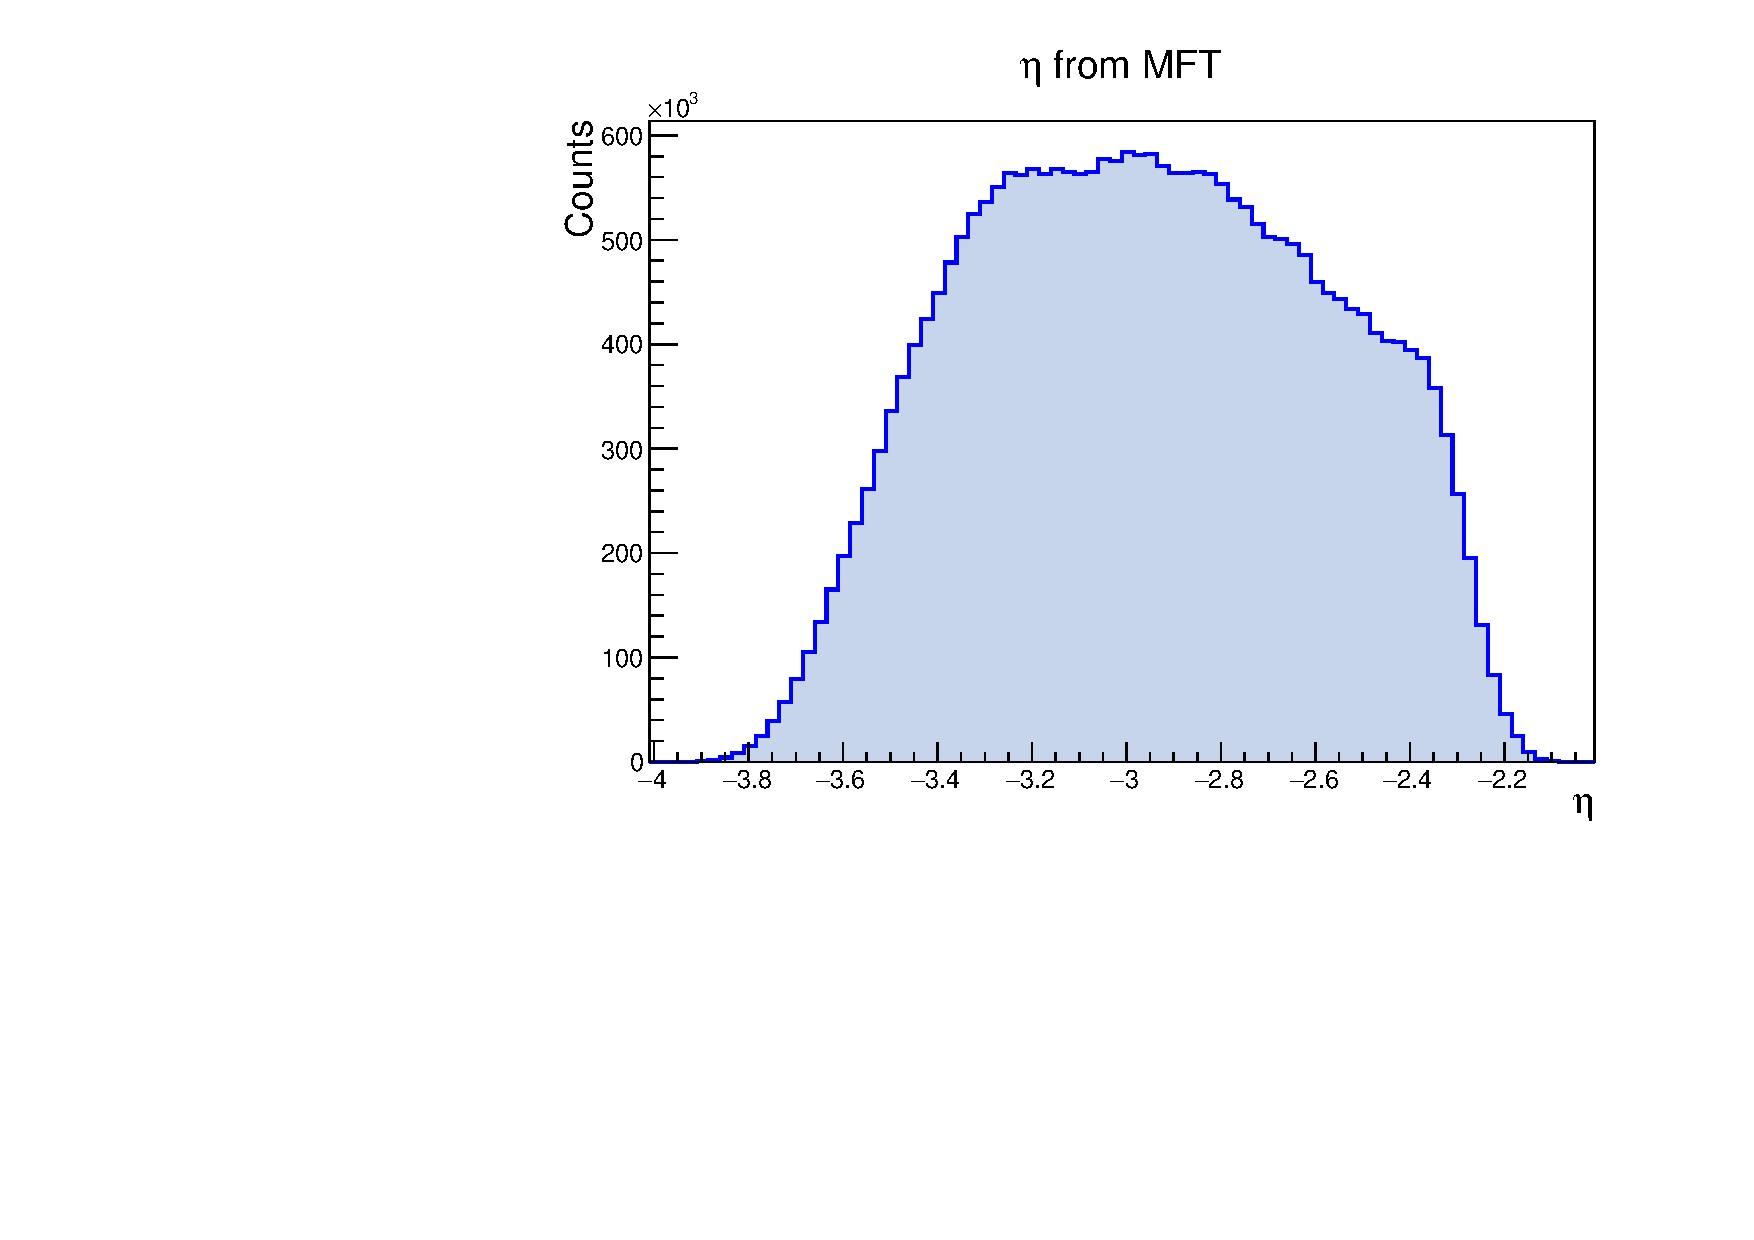
\includegraphics[width=\linewidth]{Plots/pass3_MFT/MFTeta_pass3.pdf}
        \caption{$\eta$ of tracks detected in the MFT. }
        \label{fig:MFTeta_pass3}
    \end{subfigure}
    \hfill
    \begin{subfigure}[t]{.49\linewidth}
        \centering
        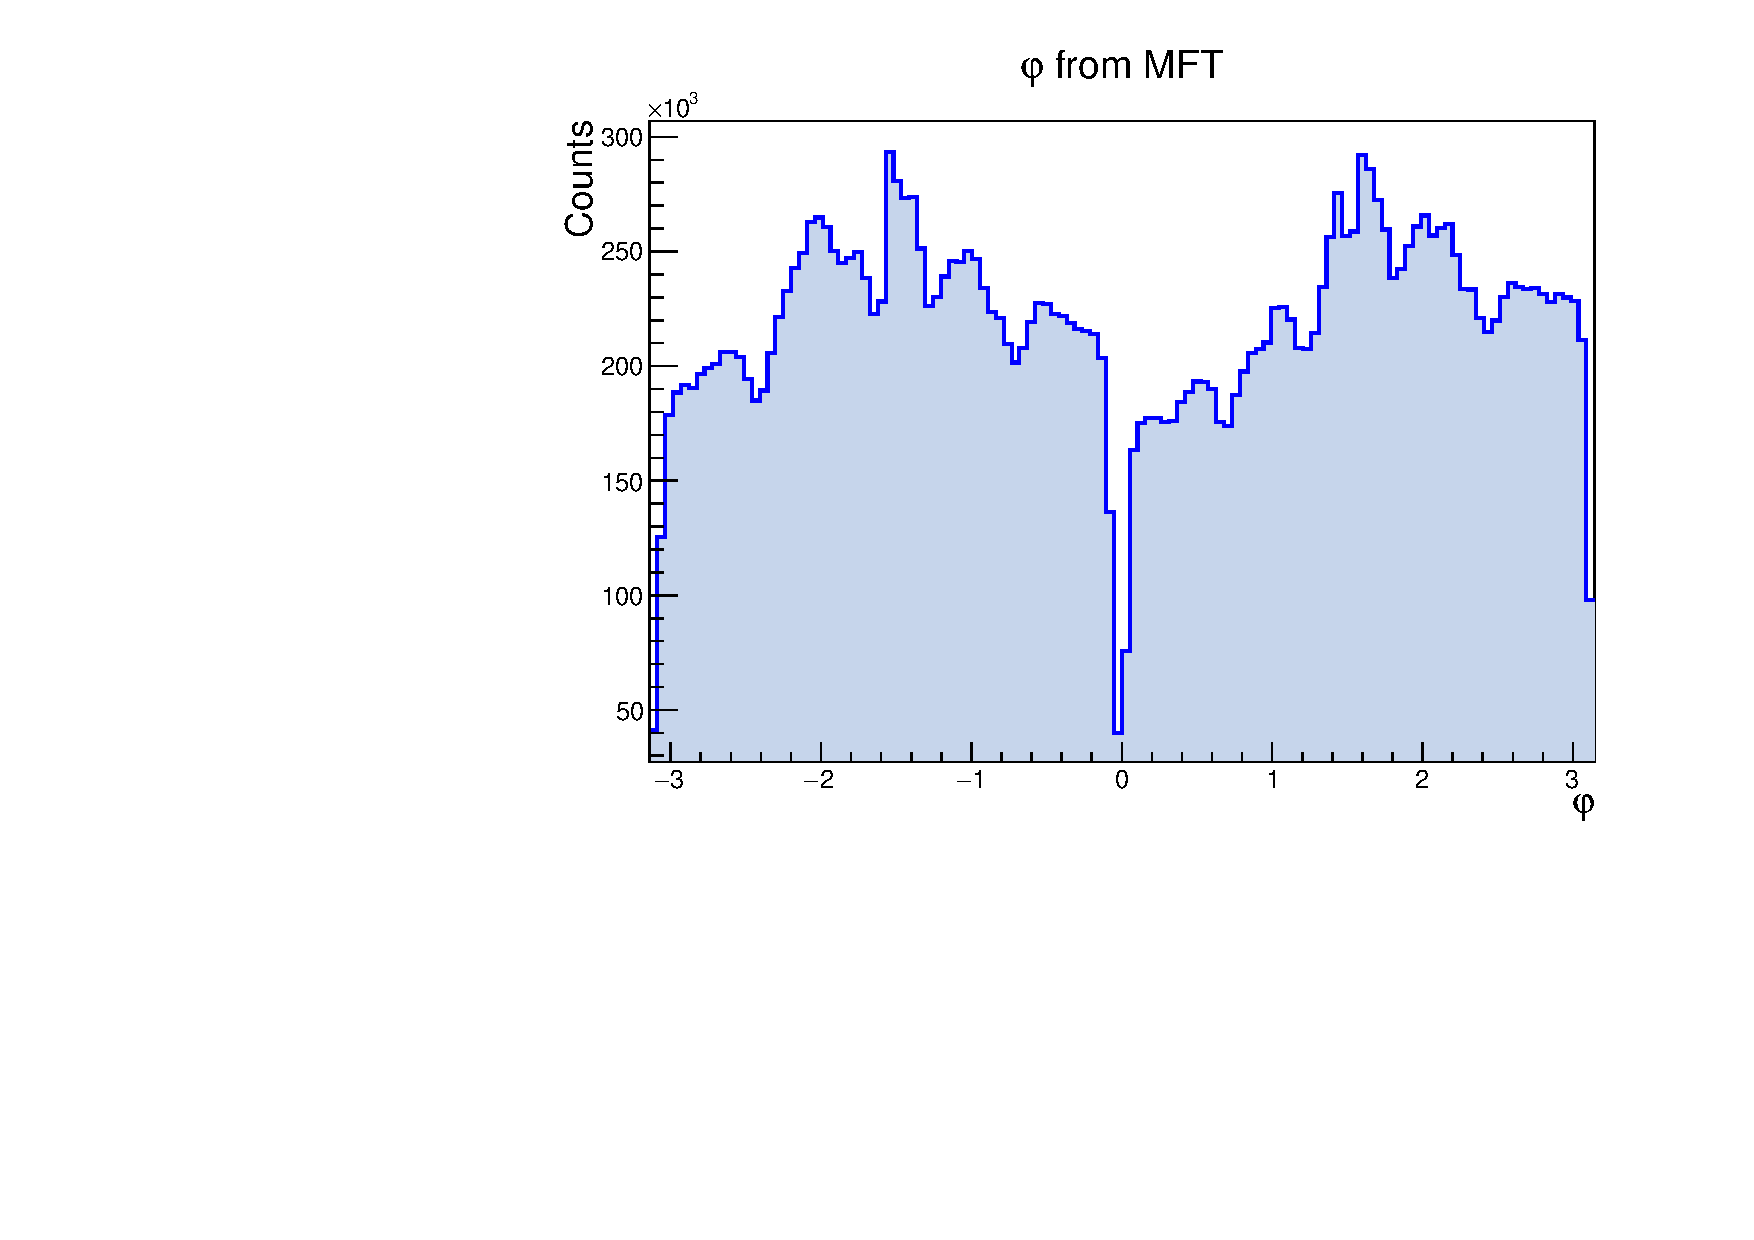
\includegraphics[width=\linewidth]{Plots/pass3_MFT/phi_pass3.pdf}
        \caption{$\varphi$ of tracks detected in the MFT. Note the range of $\varphi$.}
        \label{fig:MFTphi_pass3}
    \end{subfigure}
    \begin{subfigure}[t]{.49\linewidth}
        \centering
        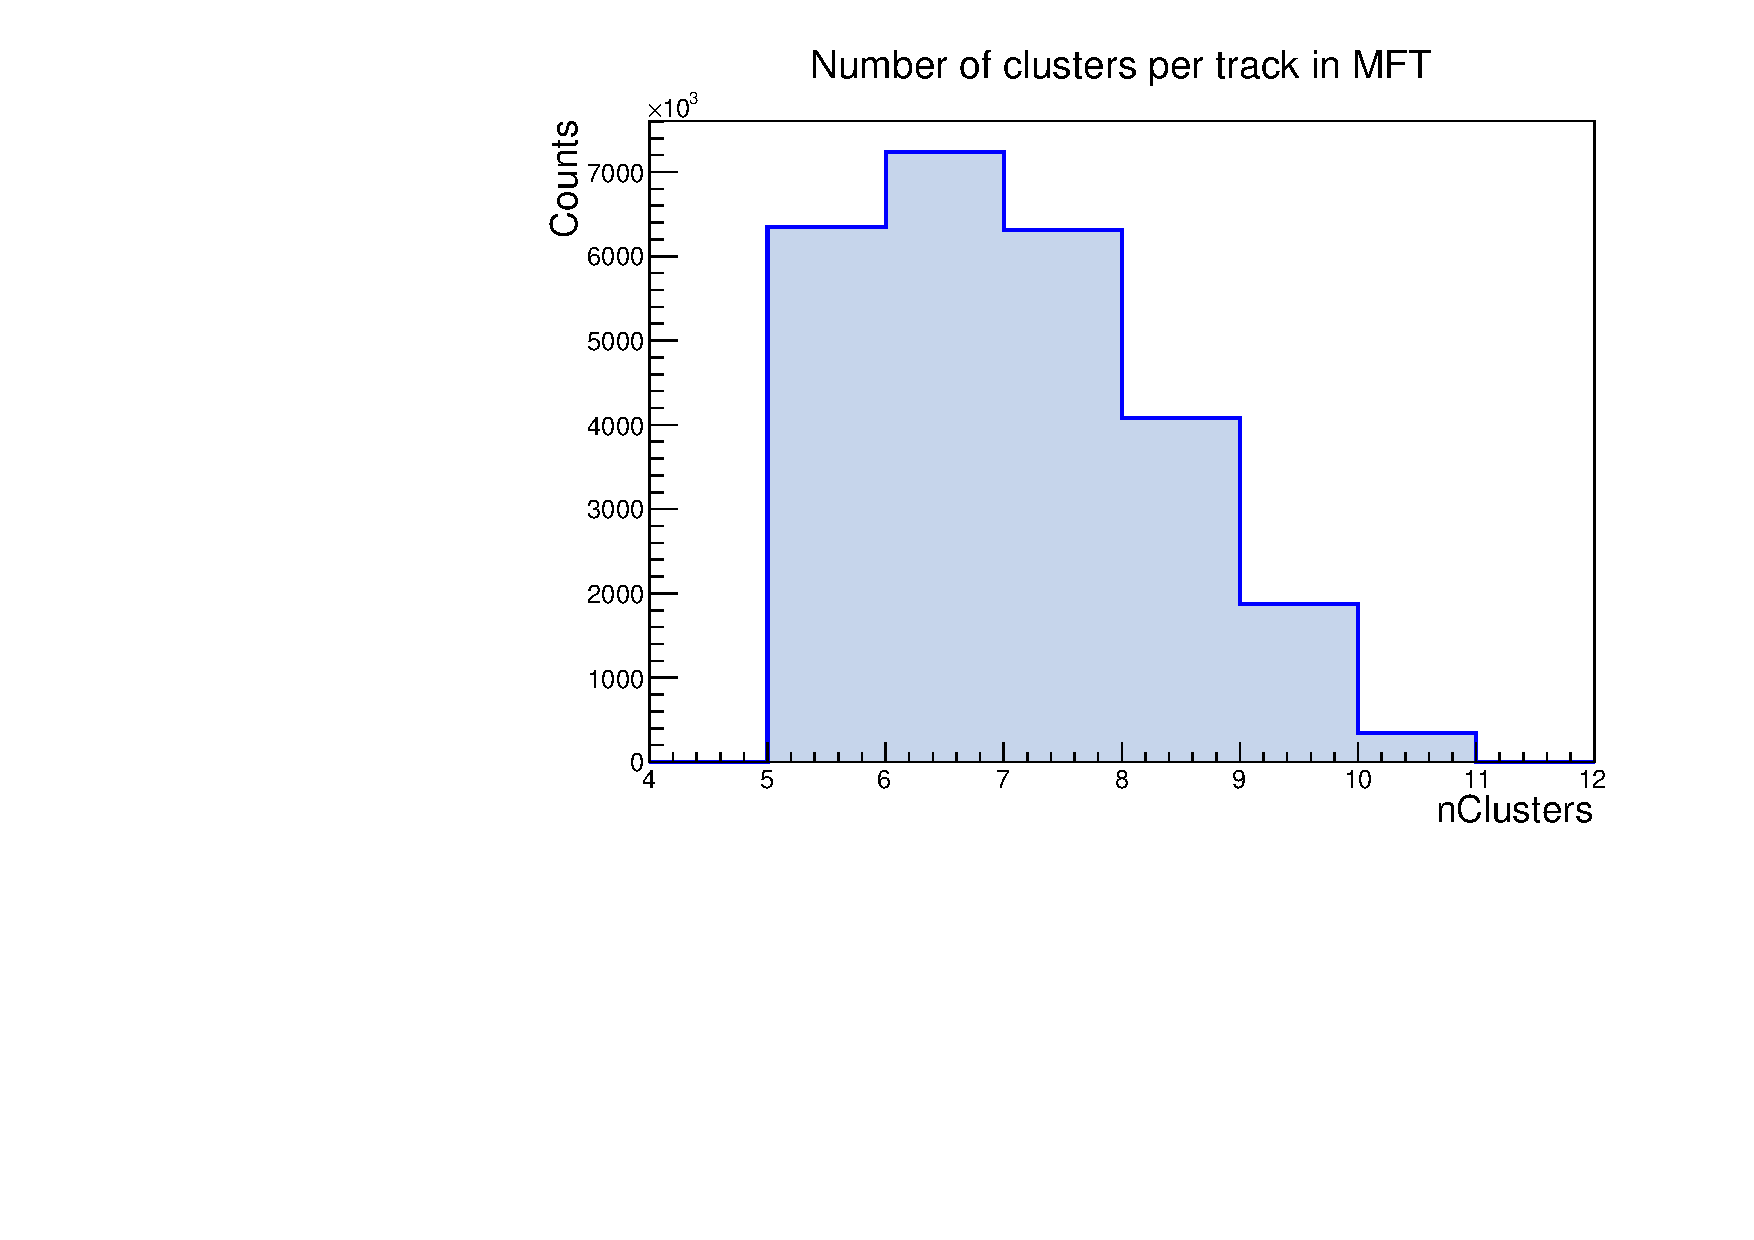
\includegraphics[width=\linewidth]{Plots/pass3_MFT/nClusters_pass3.pdf}
        \caption{Number of clusters per track detected in the MFT. Note the cut-off at 5.}
        \label{fig:MFTnClusters_pass3}
    \end{subfigure}
    \hfill
    \begin{subfigure}[t]{.49\linewidth}
        \centering
        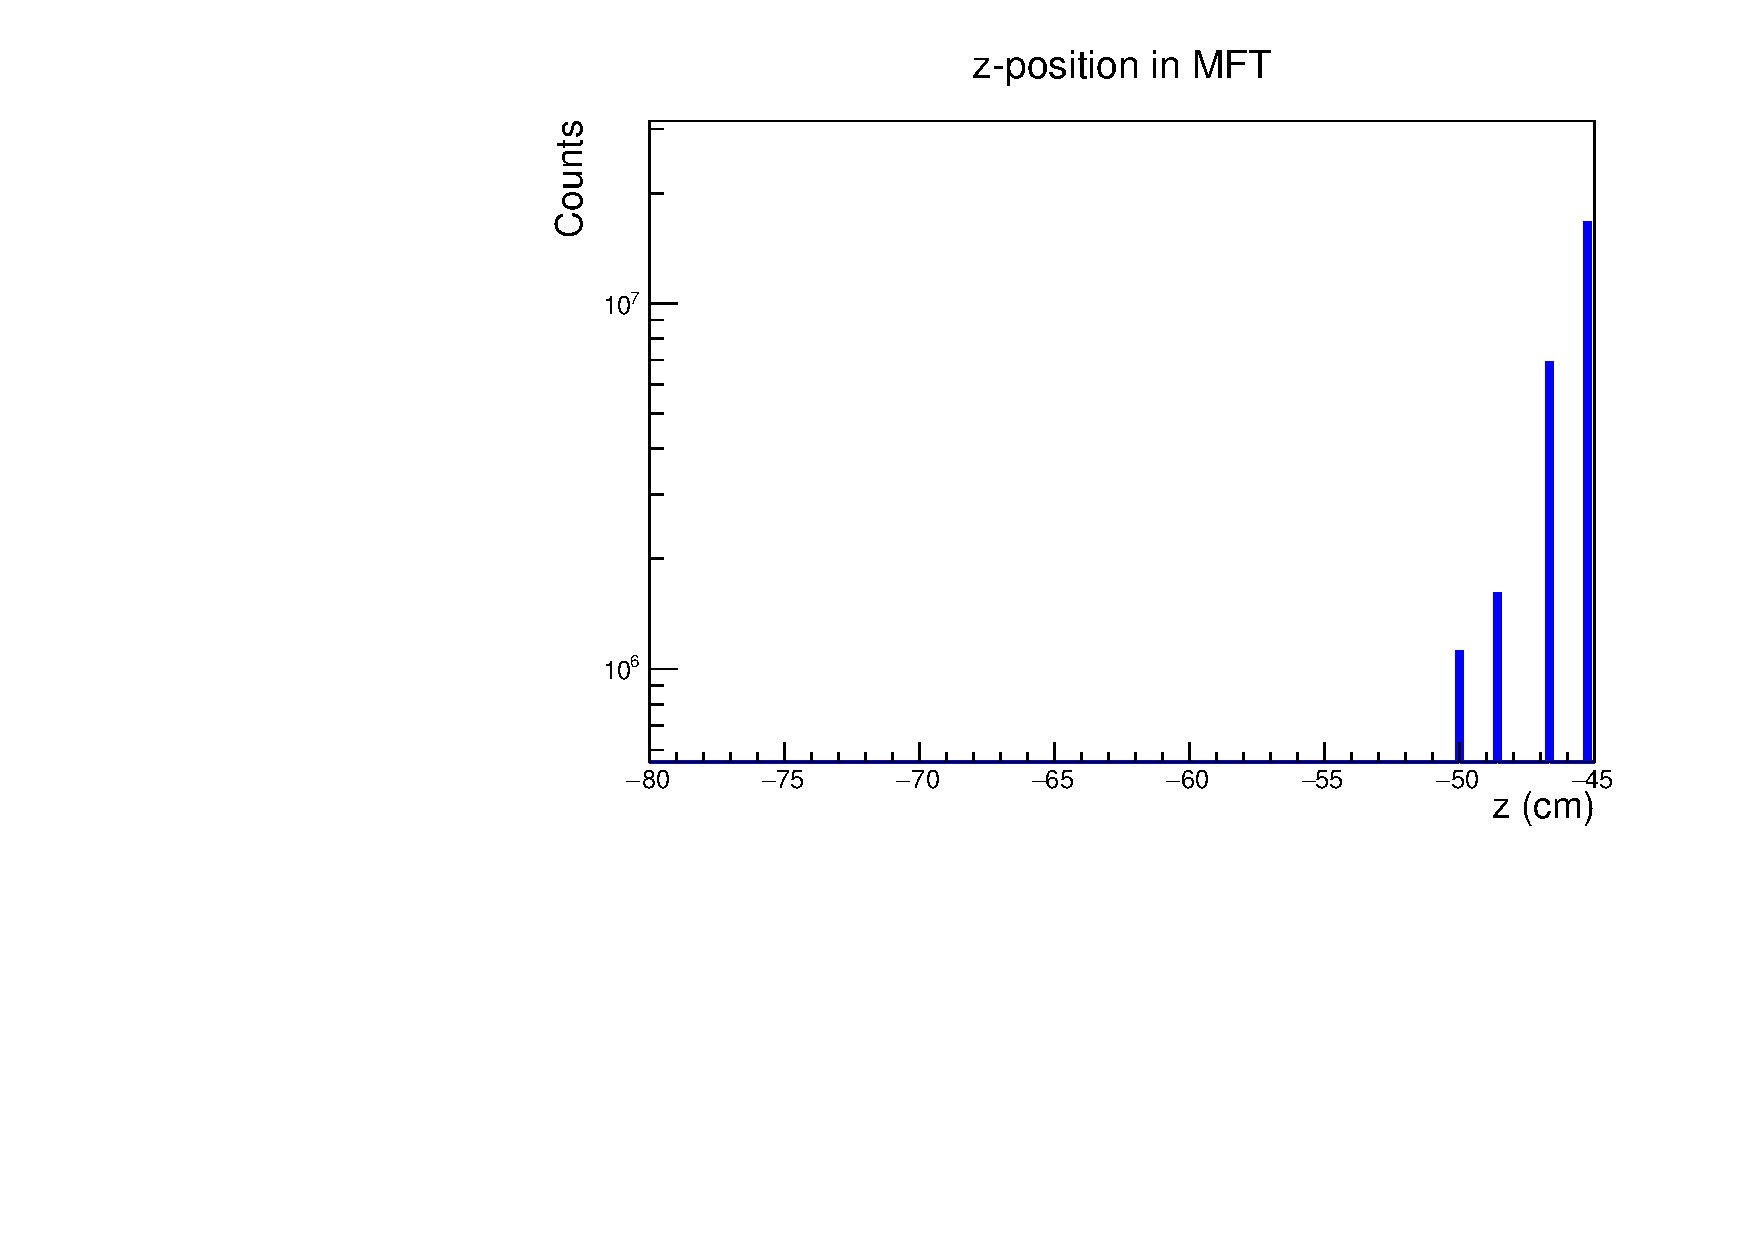
\includegraphics[width=\linewidth]{Plots/pass3_MFT/Z_MFT_pass3.pdf}
        \caption{$z$-position of first hit in the MFT. Note how the $z$ range covers the whole MFT but only the first 4 detector planes have hits.}
        \label{fig:Z_MFT_pass3}
    \end{subfigure}
\caption[Gistograms of $\eta$, $\varphi$, \OldTexttt{nClusters}, and $z$ for tracks from pass 3 in the MFT]{1-D histograms for some kinematic variables as well as the number of clusters per track in the MFT. Data from reconstruction pass 3. }
\label{fig:MFT_1D_pass3}
\end{figure}

In the AOD data model there is a table called \texttt{MFTTracks} which contains the tracks detected in the MFT. When we began this analysis, only two reconstruction passes had been run on the data and while the MFT was switched on for the runs, the \texttt{MFTTracks} table had not been populated. We thus had to wait for pass 3 and we spent that time getting familiar with the analysis framework as described in \cref{sec:AnalysingWithO2}. With pass 3 available, the plots in \cref{fig:MFT_1D_pass3} were able to be created. The variables plotted are all available as static or dynamic columns in the AOD structure so no complicated analysis was needed to obtain them. 

Starting with $\eta$, we see the distribution is lopsided to the lower $\eta$ values but it's not as smooth in the middle as we might expect from a detector with continuous sensitive material in those regions. We will investigate this more in \cref{sec:Comparing}. The $\varphi$ plot shows the structure of the MFT quite well. The valley at the centre shows the gap between the top and bottom half-disks and the spikes come from the fact that the sensitive area of each disk is not perfectly circular, so there will be directions that can detect more tracks than others. 

The number of clusters per track is interesting. As was mentioned in \cref{sec:MFT_Theory}, the MFT requires a track to be detected in 4 out of the 5 disks, by default, in order to be considered a track. The translation of that statement into number of clusters per track is a bit unclear but we might expect that the minimum number of clusters per track should be 4 as each disk has 2 planes but the track only needs to have a cluster in one of them to count towards the 4 out of 5. However, what we see in \cref{fig:MFTnClusters_pass3} is a minimum of 5 clusters per track. This might be down to a choice made in the reconstruction process to instead require that all 5 disks detect the track before it is accepted. It could also be due to a physical limitation where it's simply not possible for 4 disks to detect a track and not see clusters in 5 disks. At the point of writing, we have not been able to determine the reason for this as the details of reconstruction are near impossible to find.

Interpreting \cref{fig:Z_MFT_pass3} was its own adventure. The documentation for the AOD data model is unclear about what gets calculated for the $z$ column in the \texttt{MFTTracks} table, but we believe that it represents the $z$-position of the first hit (or cluster) of a given track in the MFT. We see that after the fourth plane, i.e. the second disk, there is no data. This supports the fact that 4 out of 5 disks are required to accept a track as having a first hit in the third disk will obviously never result in a track hitting 4 disks. This information seems to be contradicting the information from \cref{fig:MFTnClusters_pass3} but we regrettably have no resolution to the situation.

\bigskip

Out of interest, we can look at the $x$ and $y$ positions of the hits in the first 4 layers that we saw in \cref{fig:Z_MFT_pass3}. This is shown in \cref{fig:MFT_x_y_pass3} and the structure of the ladders of pixel detectors can clearly be seen. As with the $z$ plot, there is no further data for the other layers in the MFT. It would be useful to be able to see the positions of all of the hits for a track, but we are restricted to what is added to the AOD and at this point, this is all we have to work with. 

The blank regions in the $x$-$y$ plots are likely areas where the data has been masked. This is most likely to be because the detector had high noise levels in those areas, which would blow out the rest of the data. Looking at the first two plots, we can see how the front and back planes of the first disk are offset from each other, as we saw in \cref{fig:MFT_Disk4_mapping}. We also see an increased number of hits closer to the centre of the disks. This can be explained by the fact that, assuming particles are emitted isotropically from the IP, there will be a drop-off in density of particles as the distance from the IP increases and since the disks are flat, the larger the radius on the disk, the further its outer points are from the IP. Thus the density of hits should decrease as the disk radius increases. 

\bigskip

The last interesting plot from reconstruction pass 3 is a 2-D histogram of $\eta$ and $\varphi$. \Cref{fig:eta_phi_pass3} shows this and we can immediately see the resemblance to the layout in \cref{fig:MFT_Disk4_mapping}. As with \cref{fig:MFTphi_pass3}, we can see the gap in between the half-disks. 

\begin{figure}[H]%
    \centering
    \begin{subfigure}[t]{.45\linewidth}
        \centering
        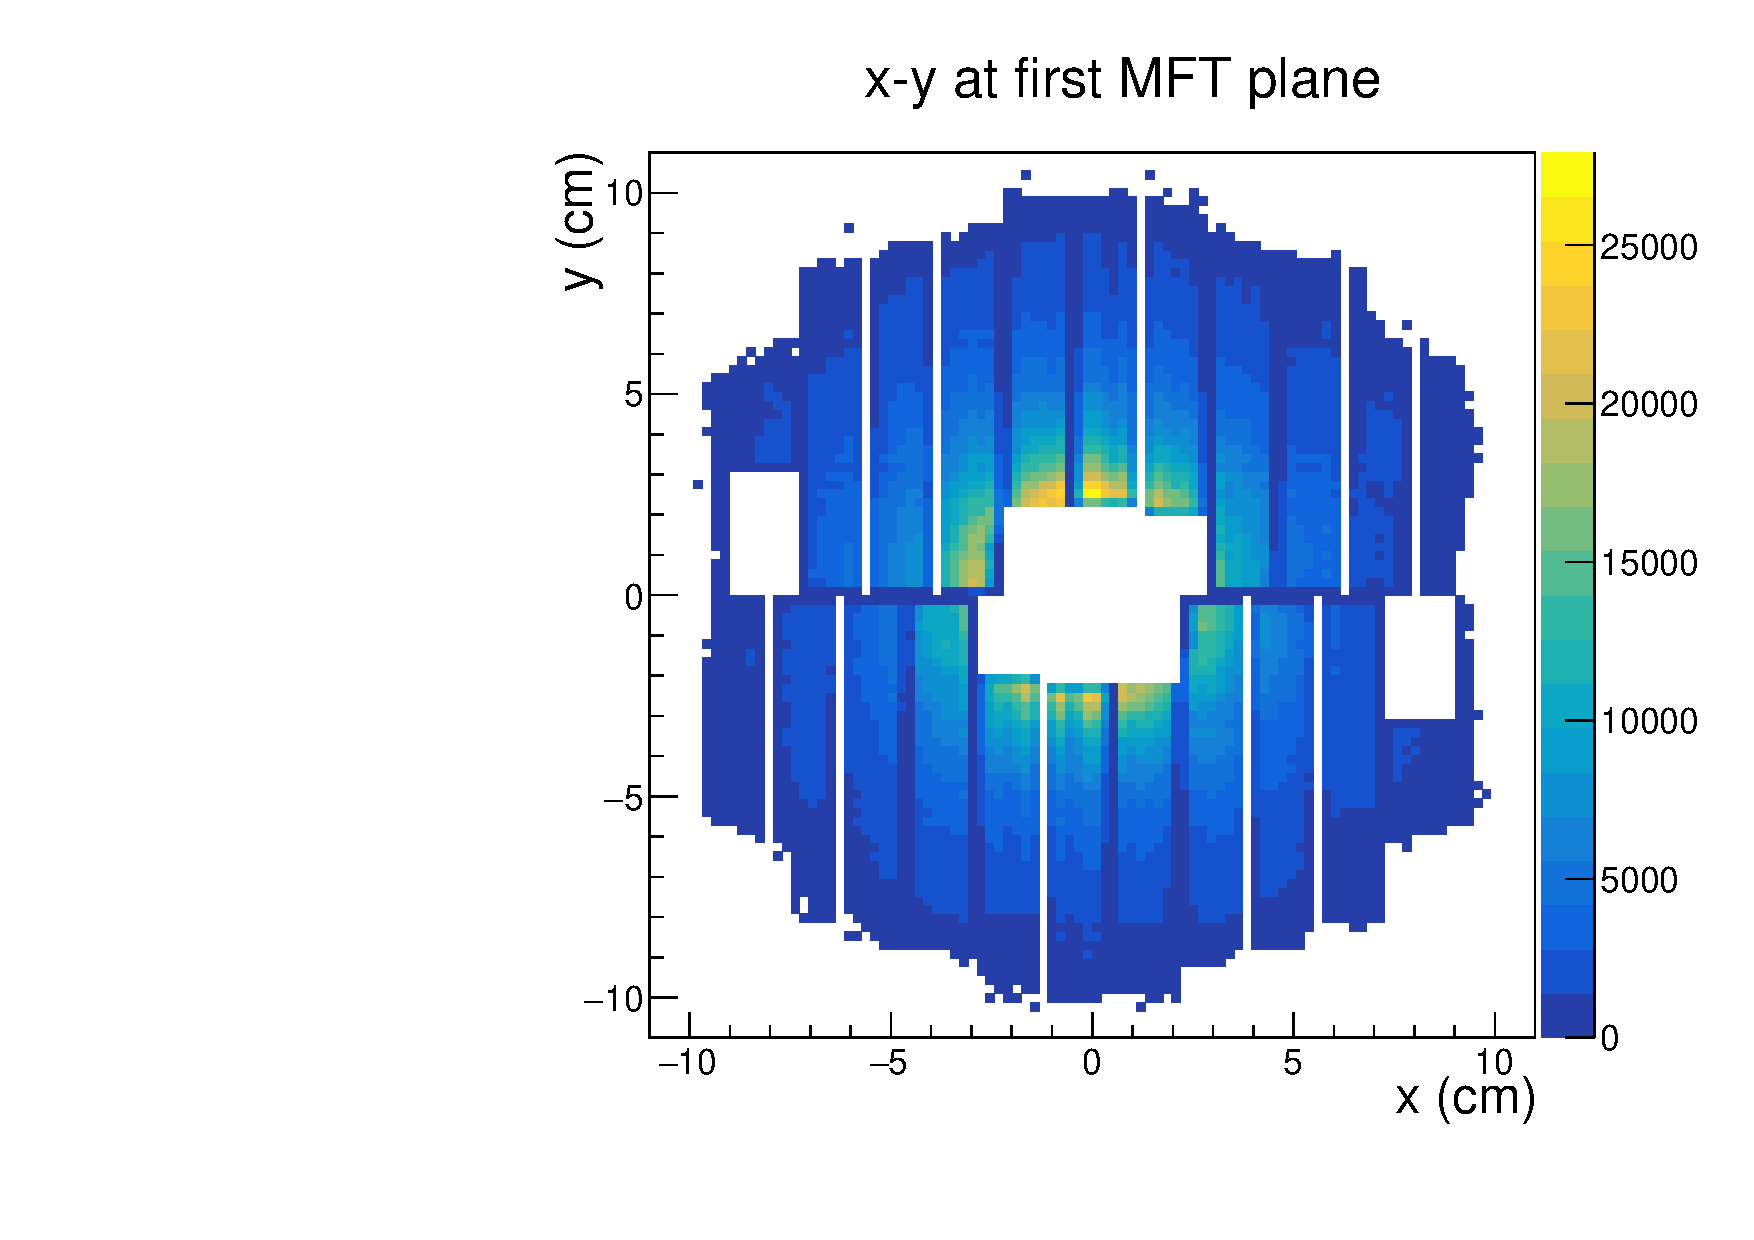
\includegraphics[width=\linewidth]{Plots/pass3_MFT/x_y_1_pass3.pdf}
        \caption{}
        \label{fig:x_y_1_pass3}
    \end{subfigure}
    \hfill
    \begin{subfigure}[t]{.45\linewidth}
        \centering
        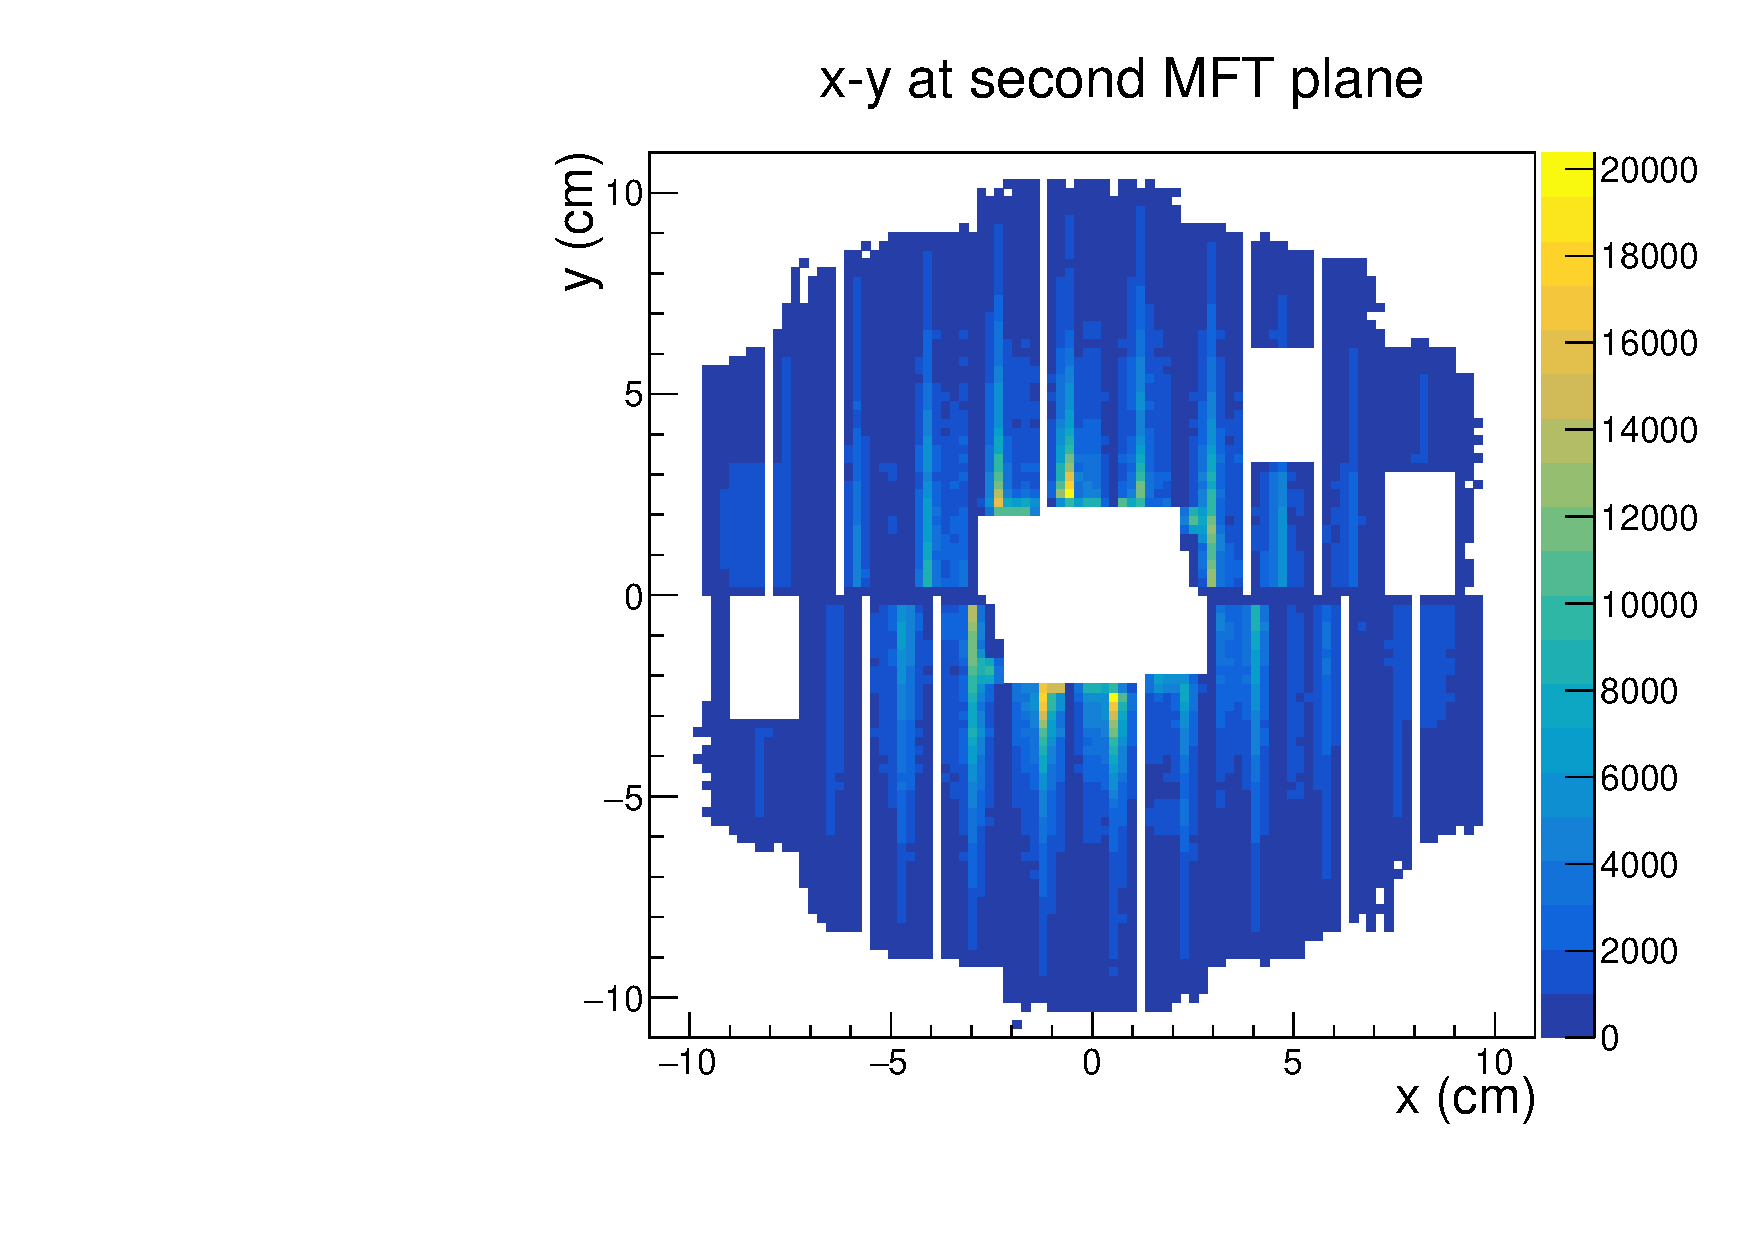
\includegraphics[width=\linewidth]{Plots/pass3_MFT/x_y_2_pass3.pdf}
        \caption{}
        \label{fig:x_y_2_pass3}
    \end{subfigure}
    \begin{subfigure}[t]{.45\linewidth}
        \centering
        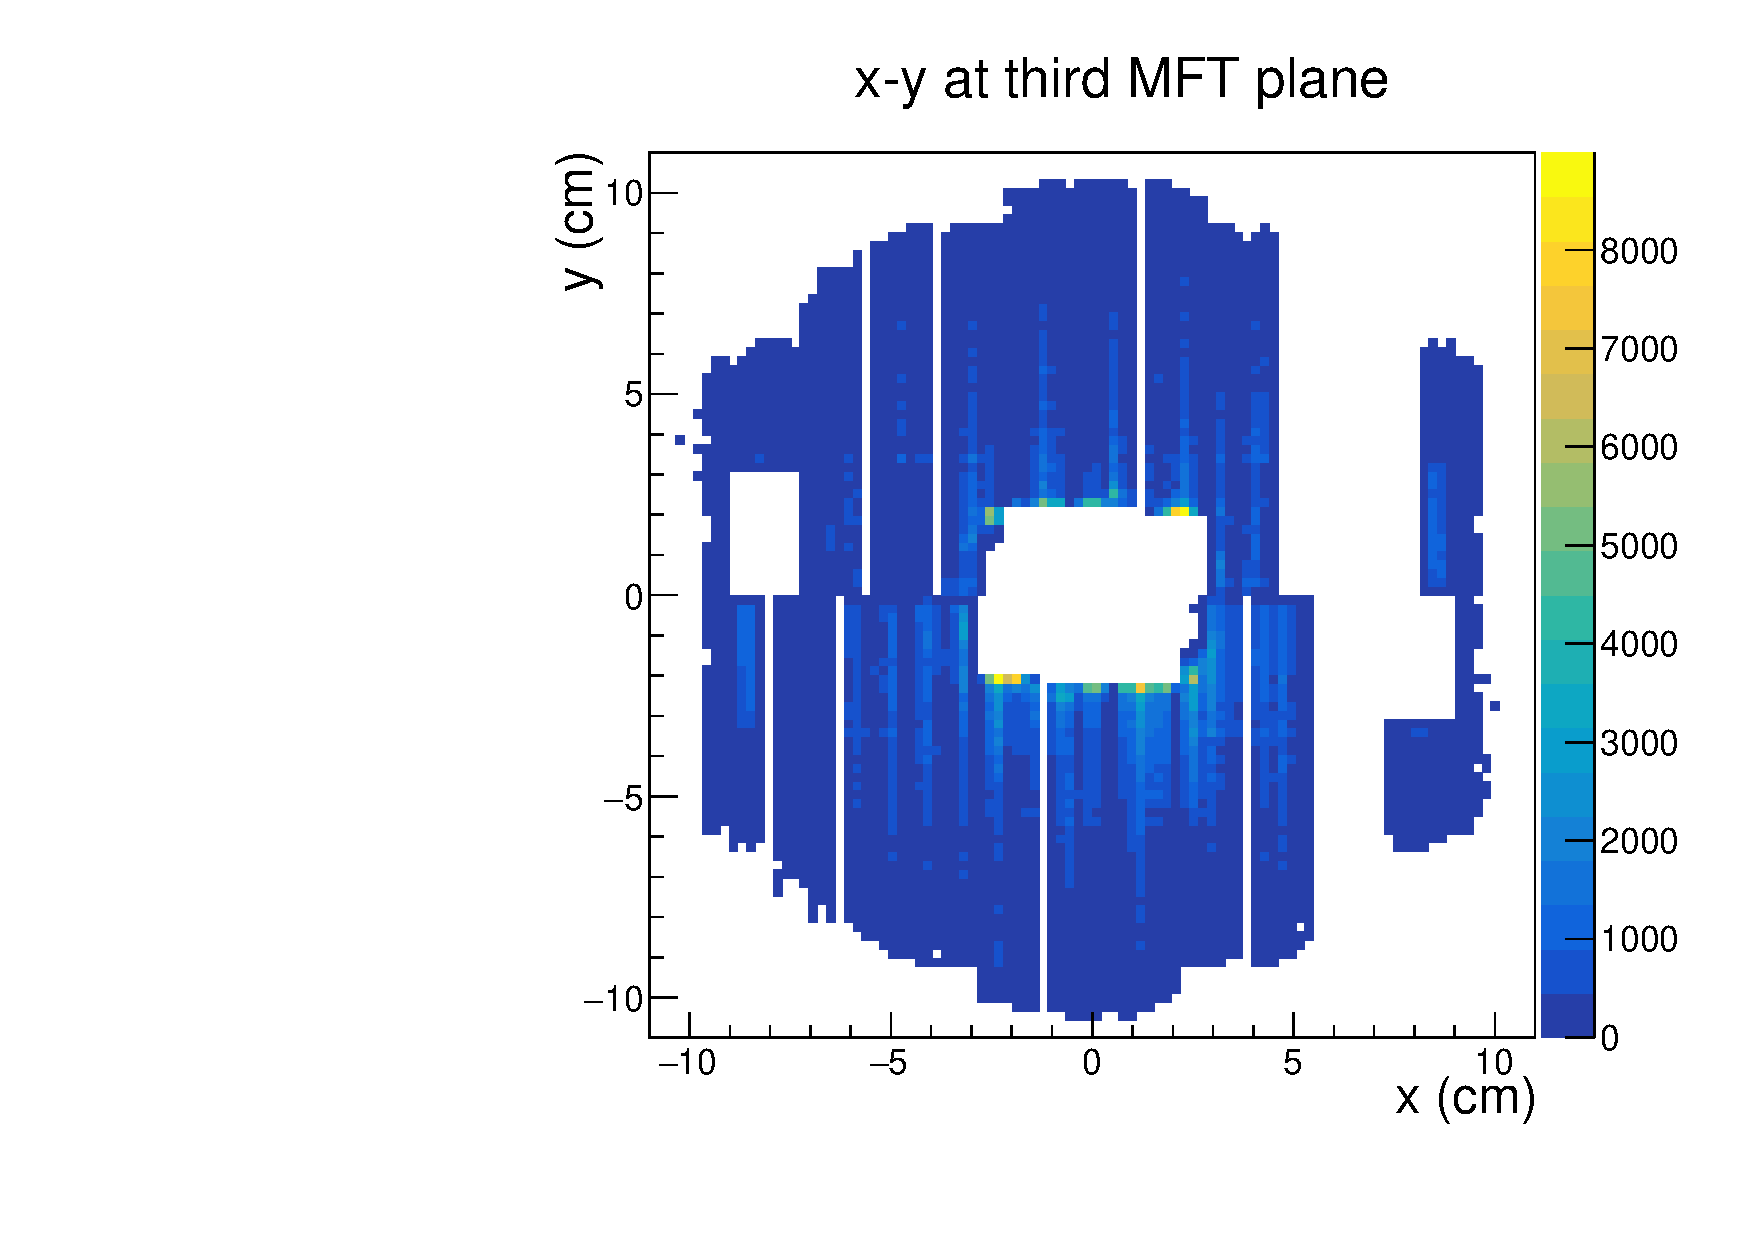
\includegraphics[width=\linewidth]{Plots/pass3_MFT/x_y_3_pass3.pdf}
        \caption{}
        \label{fig:x_y_3_pass3}
    \end{subfigure}
    \hfill
    \begin{subfigure}[t]{.45\linewidth}
        \centering
        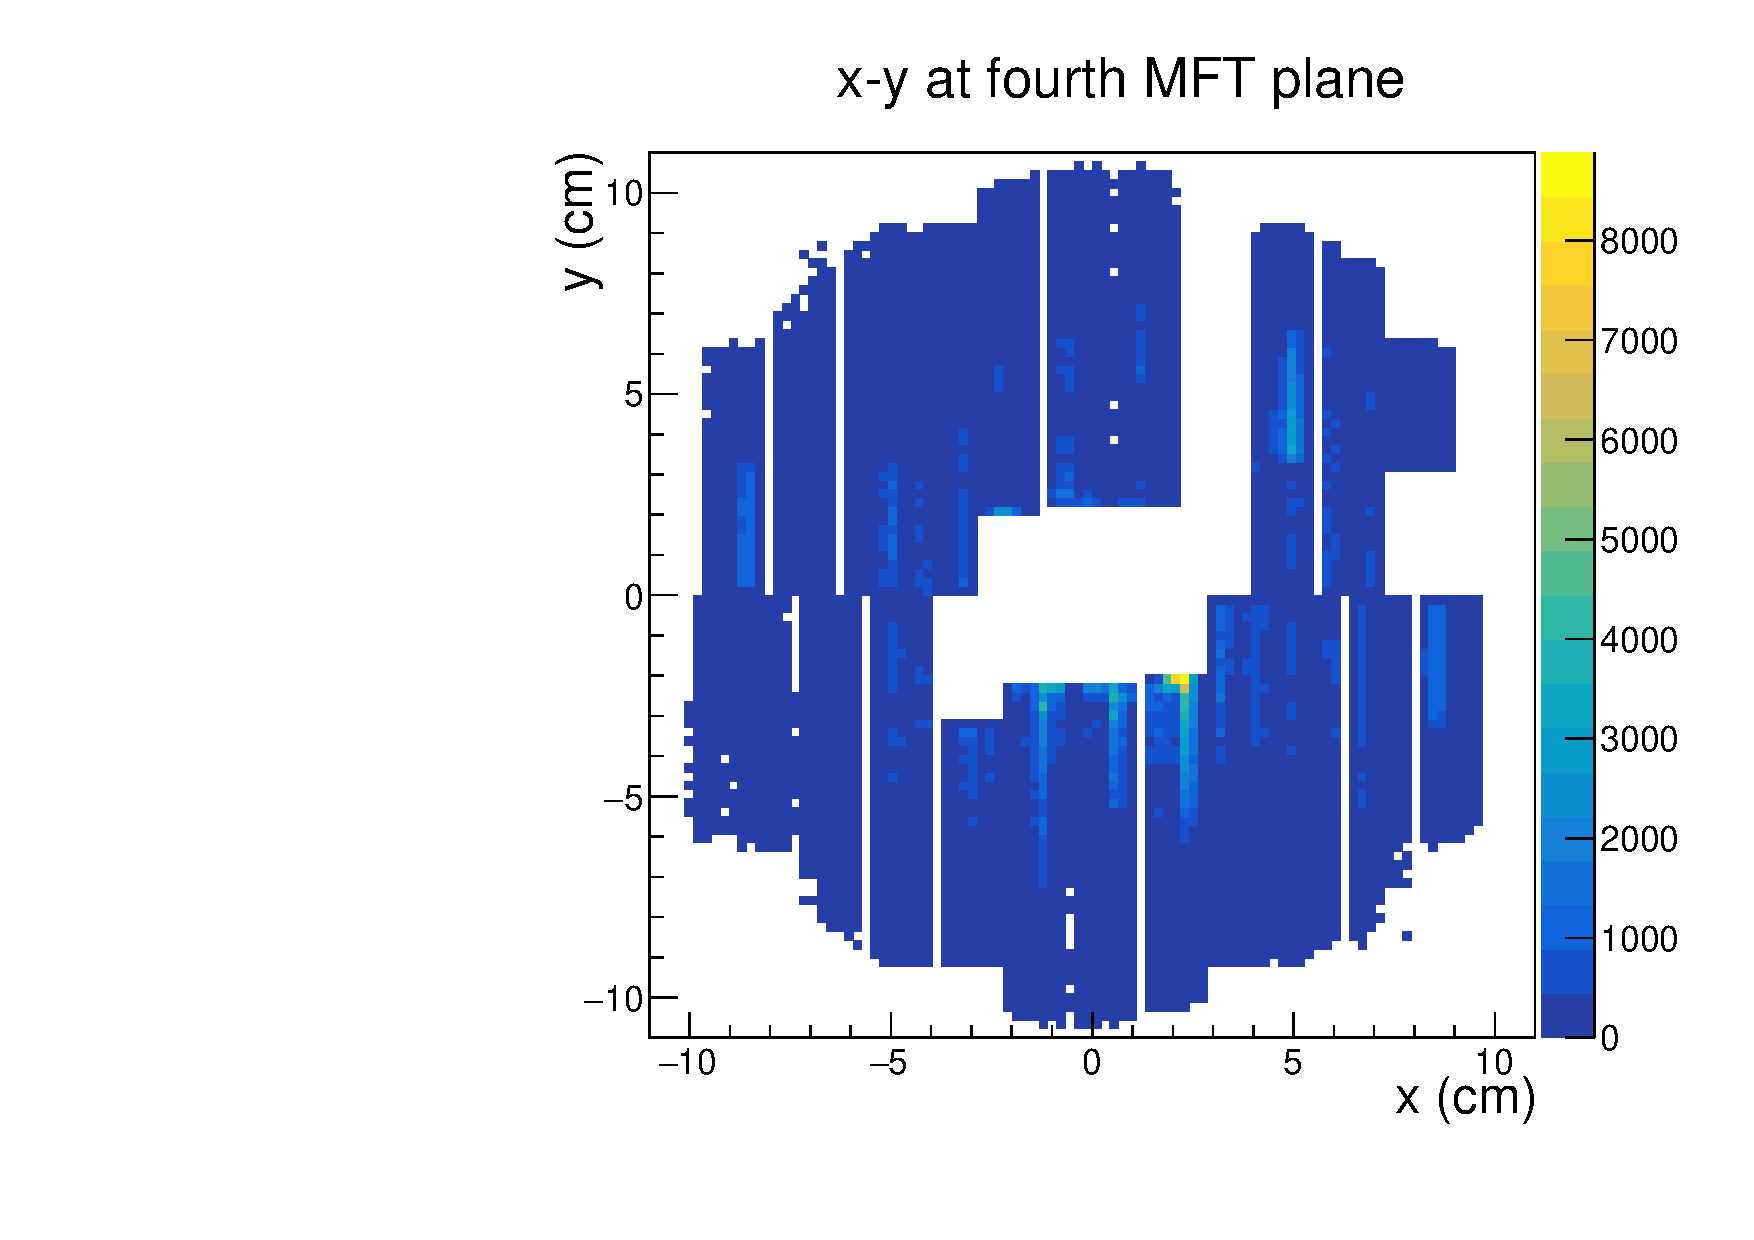
\includegraphics[width=\linewidth]{Plots/pass3_MFT/x_y_4_pass3.pdf}
        \caption{}
        \label{fig:x_y_4_pass3}
    \end{subfigure}
\caption[$x$-$y$ histograms of tracks at different planes of the MFT]{$x$ and $y$ positions of hits in the first 4 layers of the MFT. This is related to \cref{fig:Z_MFT_pass3} as these are the first hits for a given track, so looking at the later layers yields no data. The sections with no data have likely been masked out to remove regions of abnormally high noise. Important to note how at the centre of the disk we see a higher hit density than further out.}
\label{fig:MFT_x_y_pass3}
\end{figure}

\begin{figure}[h]
    \begin{center}
        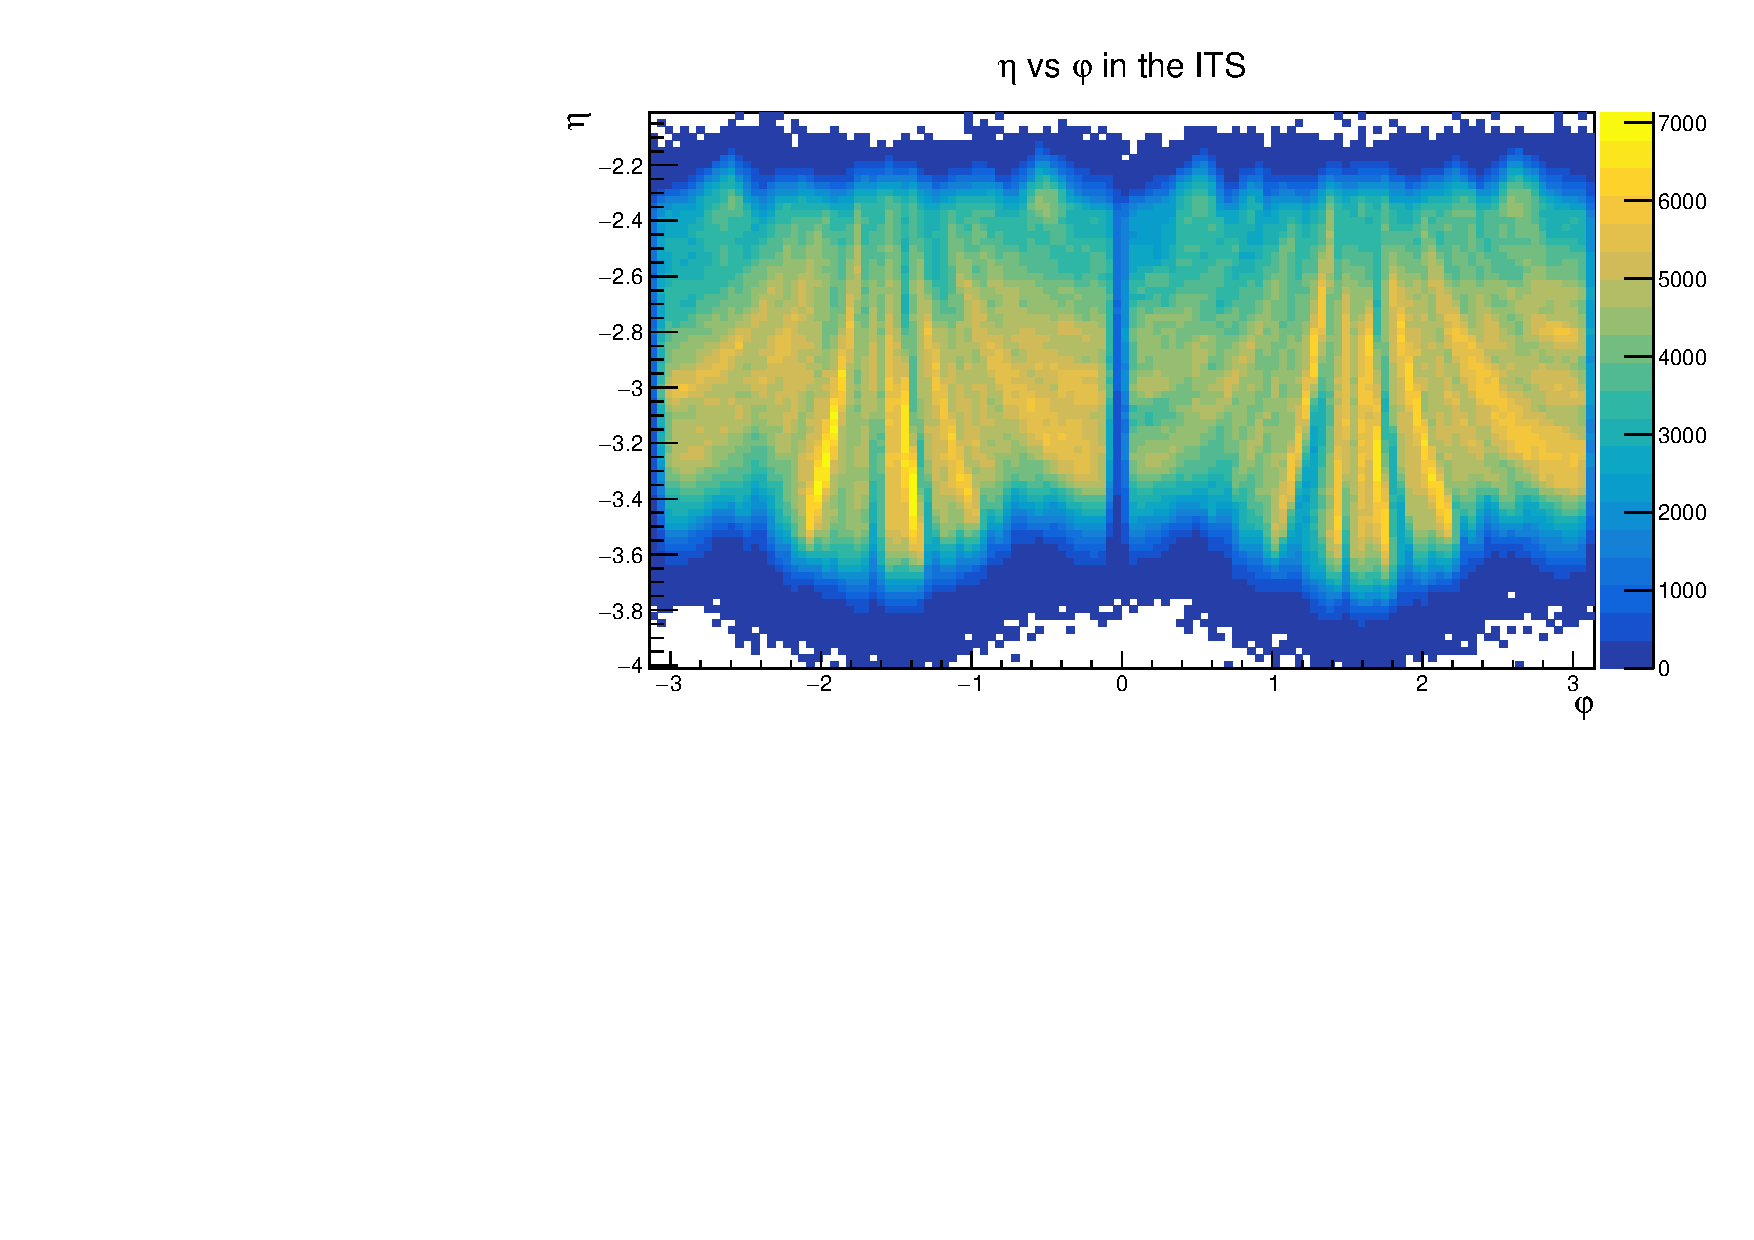
\includegraphics[width=.8\textwidth]{Plots/pass3_MFT/eta_phi_pass3.pdf}
        \caption[$\eta$-$\varphi$ histogram for tracks from pass 3 in the MFT]{Histogram of $\eta$ and $\varphi$ for tracks in the MFT from reconstruction pass3. The half-disk structure can clearly be seen when comparing to \cref{fig:MFT_Disk4_mapping}. }
        \label{fig:eta_phi_pass3}
    \end{center}
\end{figure}

\subsection{Comparing pass 3 to pass 4}\label{sec:Comparing}
In \cref{fig:MFTeta_pass3} we can see that the distribution looks slightly jagged from about -2.4 to -3.4, especially when compared to the section between -3.4 and -4. There isn't any reason to expect a non-smooth distribution there, and that viewpoint is supported by looking at the distribution after reconstruction pass 4. Some issues were identified with pass 3 so pass 4 was performed and we have plotted the two $\eta$ distributions in \cref{fig:pass3_pass4_eta} for comparison.

\begin{figure}[H]
    \begin{center}
        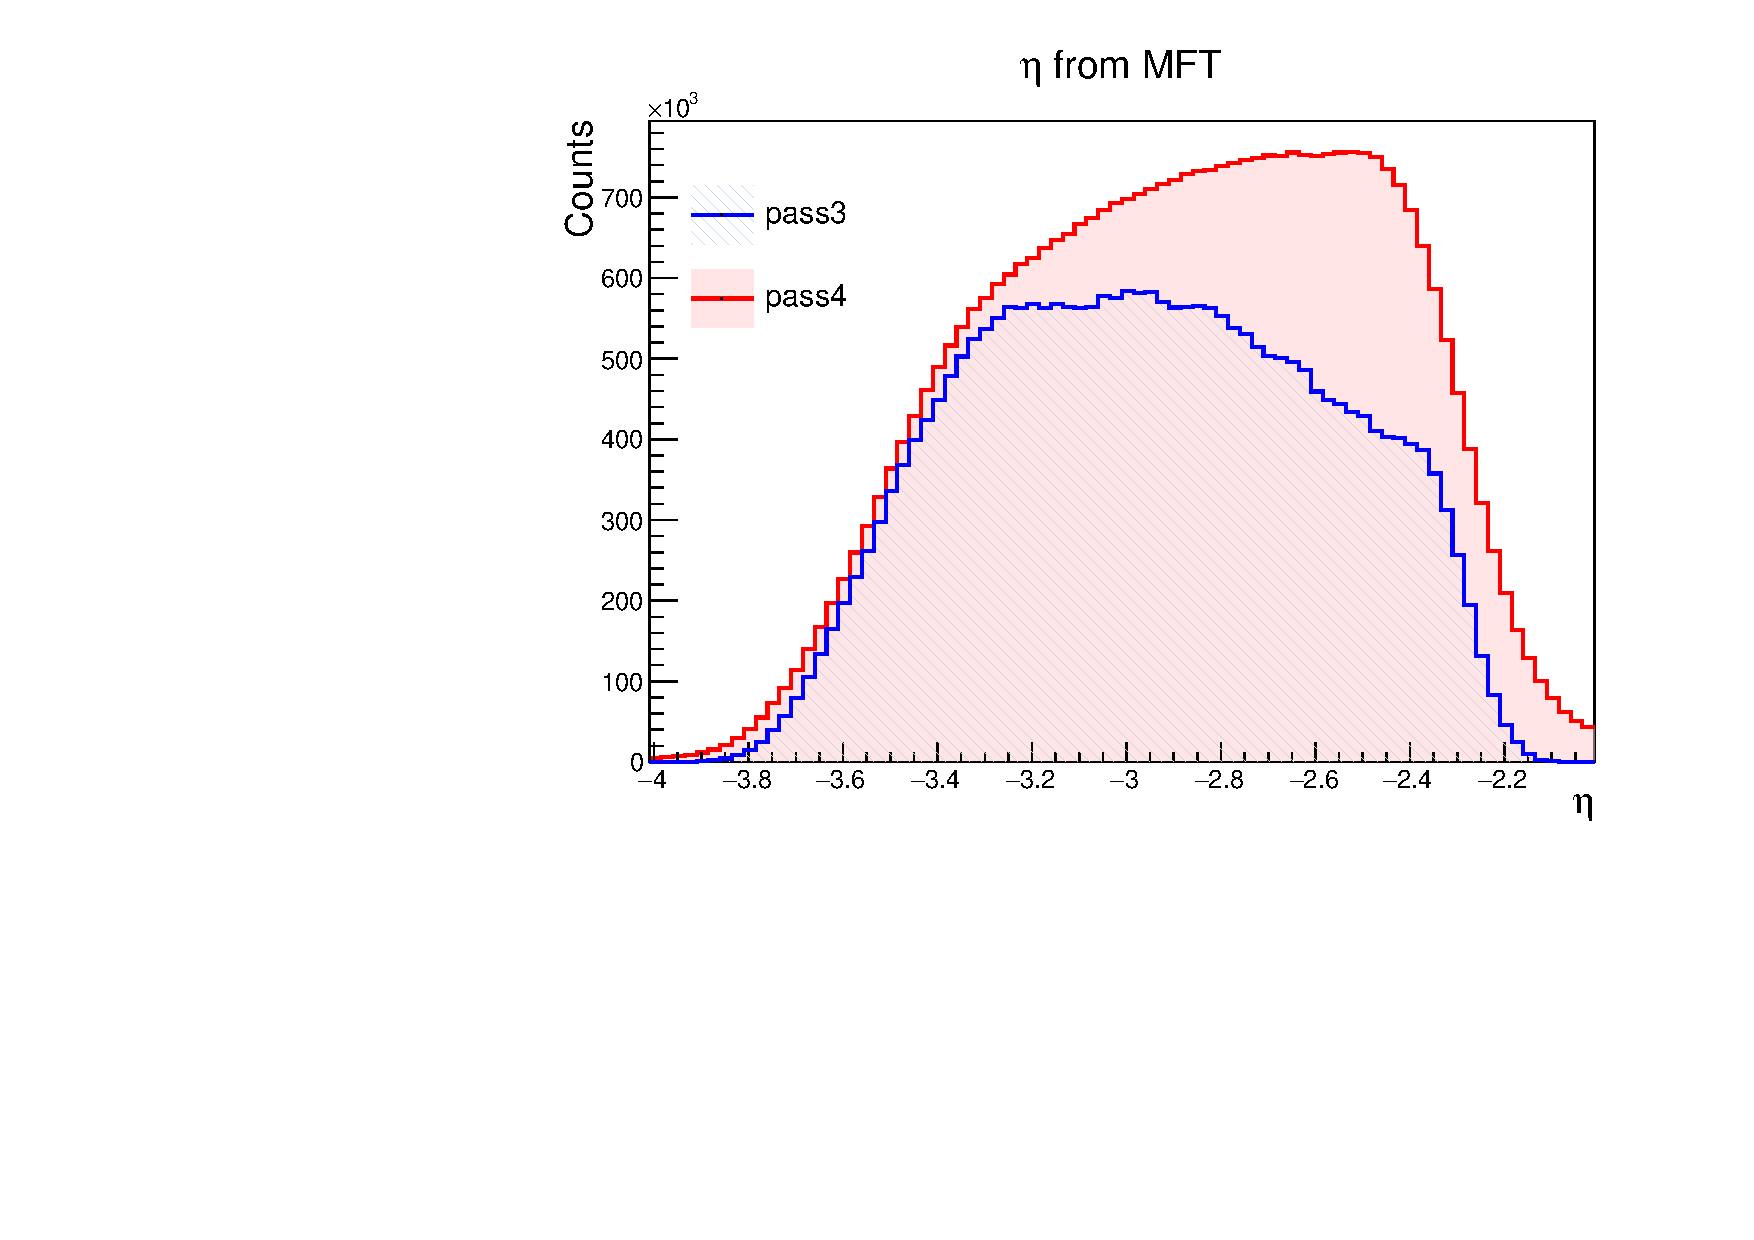
\includegraphics[width=.8\textwidth]{Plots/pass3_pass4.pdf}
        \caption[Comparison of $\eta$ distributions of tracks from pass 3 and pass 4 in the MFT]{Comparison of the distribution of $\eta$ per track for reconstruction pass 3 and pass 4. We notice that there is an overall increase in number of tracks, as well as a large number of tracks added in one region, leading to an overall more smooth distribution in pass 4. Note also how there seems to be a higher density of tracks in the smaller $\eta$ range before it drops off outside the range of the MFT.}
        \label{fig:pass3_pass4_eta}
    \end{center}
\end{figure}

What we can see in \cref{fig:pass3_pass4_eta} is that pass 3 seems to have missed a large chunk of tracks in one specific $\eta$ region compared to pass 4. The reason for this is unclear as the details of reconstruction are very hard to find but it could be due to the reconstruction now considering MCH tracks and connecting them to MFT tracks. These new tracks, and resultant $\eta$ distribution, seem to contradict the conclusion drawn from the $x$-$y$ plots in \cref{fig:MFT_x_y_pass3}, where we saw a higher density of tracks closer to the centre of the disks, i.e. with a larger rapidity. This tension is, however, resolvable through a discussion of the definition of $\eta$. We define $\eta$ in \cref{eqn:pseudorapidity} and it is very clearly a nonlinear function of $\theta$. This means that two slices of $\eta$ that have the same size will not necessarily cover the same size range of $\theta$ and since we expect tracks uniformly distributed in $\theta$, we don't necessarily expect a uniform distribution in $\eta$.

\bigskip

Lastly in comparing pass 3 to pass 4, we can have a look at the $\eta$-$\varphi$ histogram, noting the more uniform distribution overall while still showing the structure we expect from \cref{fig:MFT_Disk4_mapping}. The uniformity in the histograms for pass 4 is an indicator that the detector is working properly as we expect isotropic emission of particles from the IP. More histograms for pass 4 can be found in \cref{apx:Additional_Plots}.

\begin{figure}[h]
    \begin{center}
        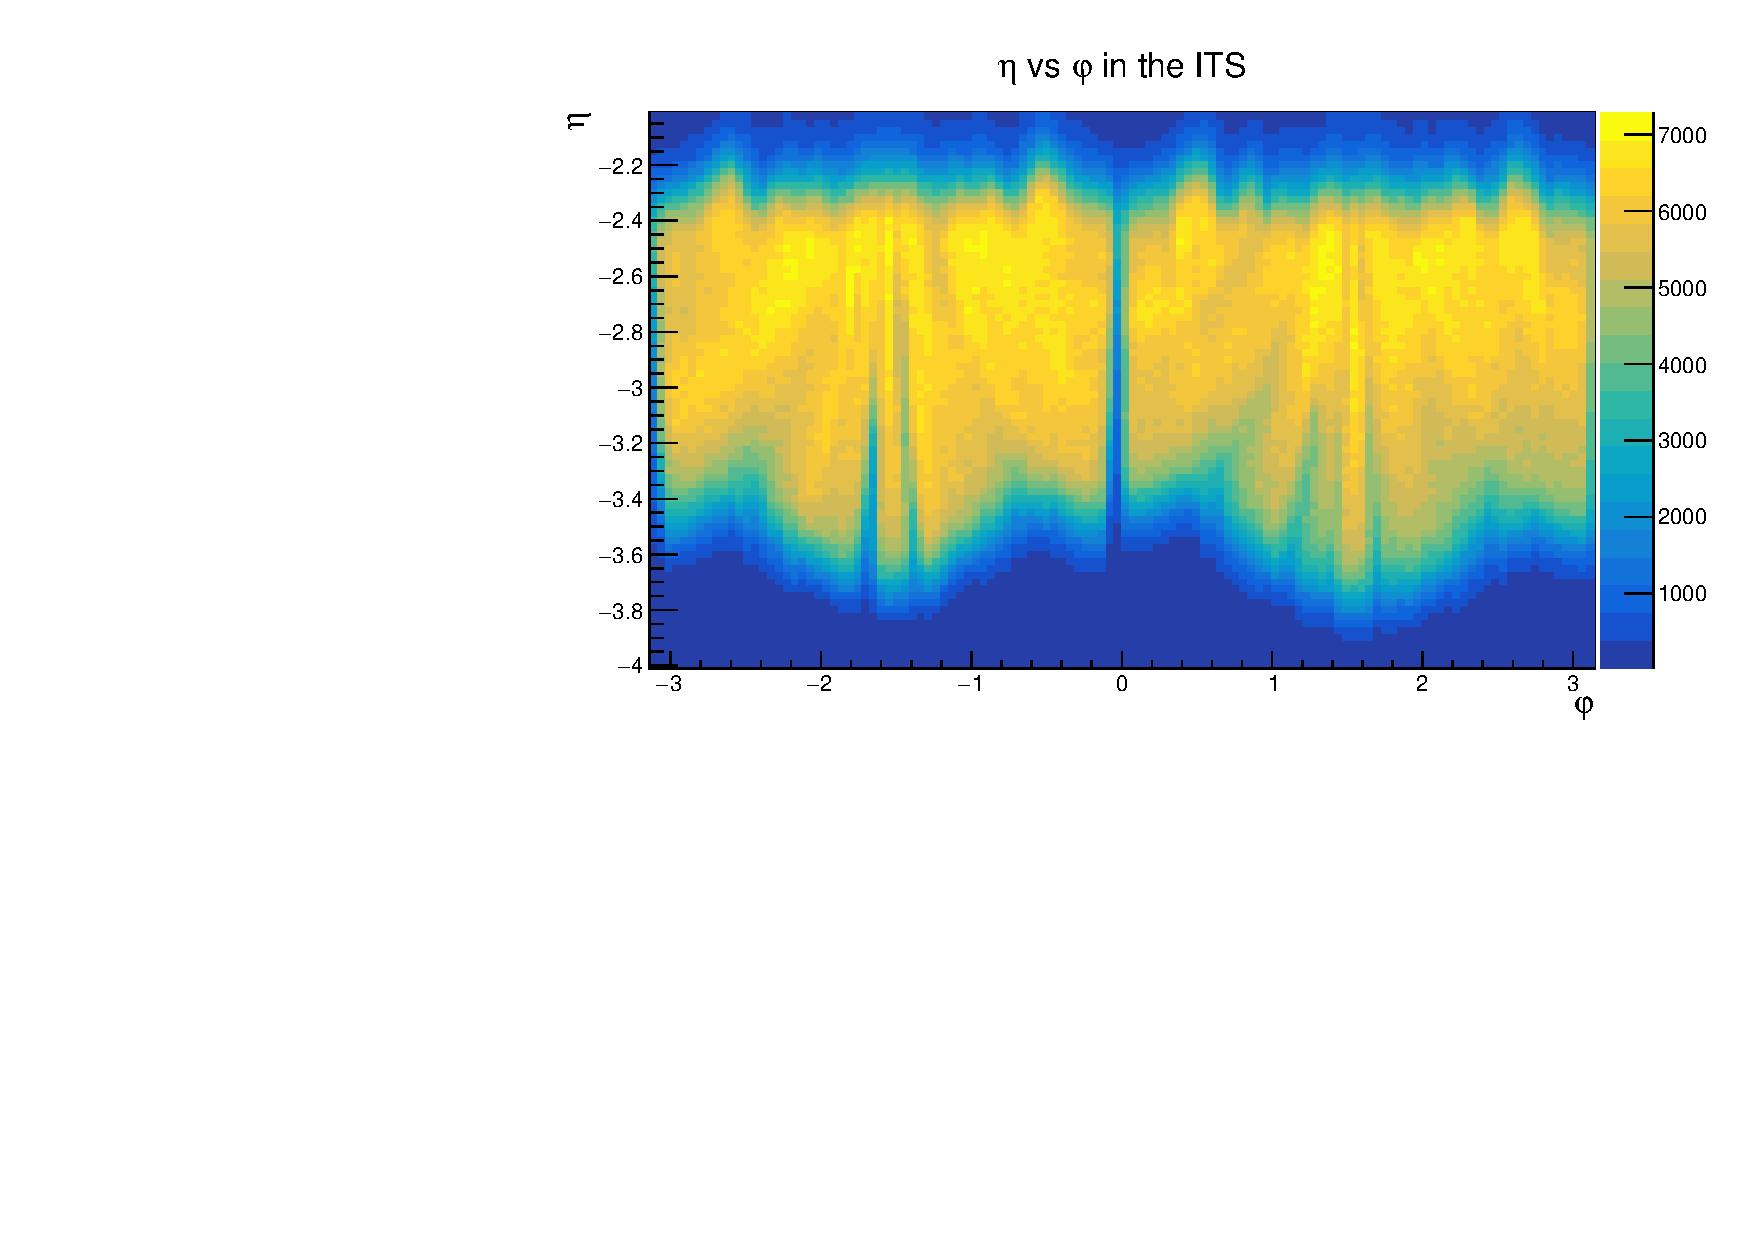
\includegraphics[width=.8\textwidth]{Plots/pass4_MFT/eta_phi_pass4.pdf}
        \caption[$\eta$-$\varphi$ histogram for tracks from pass 4 in the MFT]{Histogram of $\eta$ and $\varphi$ for tracks in the MFT from reconstruction pass 4. The overall increase in tracks can clearly be seen, as well as a more uniform overall distribution.}
        \label{fig:eta_phi_pass4}
    \end{center}
\end{figure}

\subsection{ITS Analysis}
After looking at the MFT, we turned our attention to the ITS. The first step was to look at the same variables as with the MFT. We would expect that the distributions be uniform in some sense, and unlike the MFT they should be cylindrically symmetric. The first issue, though, is making sure the data we're looking at is only coming from the ITS. The table that contains tracks from the central barrel is \texttt{aod::Tracks}, but since this has tracks as determined by all the detectors in the central barrel, such as the TPC and TOF, we had to narrow things down so we could study the ITS alone. In order to make sure only ITS tracks are considered, we used the table \texttt{aod::TracksIU} (Innermost Update) alongside the flag \texttt{hasITS}. The table returns the tracks determined at the innermost update, which is not always the ITS, so we use the \texttt{hasITS} flag to make sure that it is. This method is not foolproof but in the rigidly structured data model it was the best we could do without reworking the entire thing or undertaking the reconstruction ourselves.

\Cref{fig:ITS_1D_nohasITS} shows some histograms of the data before using the \texttt{hasITS} flag. The red histograms are without any modification and the green is choosing all tracks that are NOT seen in the ITS. These should be discussed in conjunction with the histograms of just the ITS tracks, which are presented in \cref{fig:ITS_1D}.

\begin{figure}[h]%
    \centering
    \begin{subfigure}[t]{.49\linewidth}
        \centering
        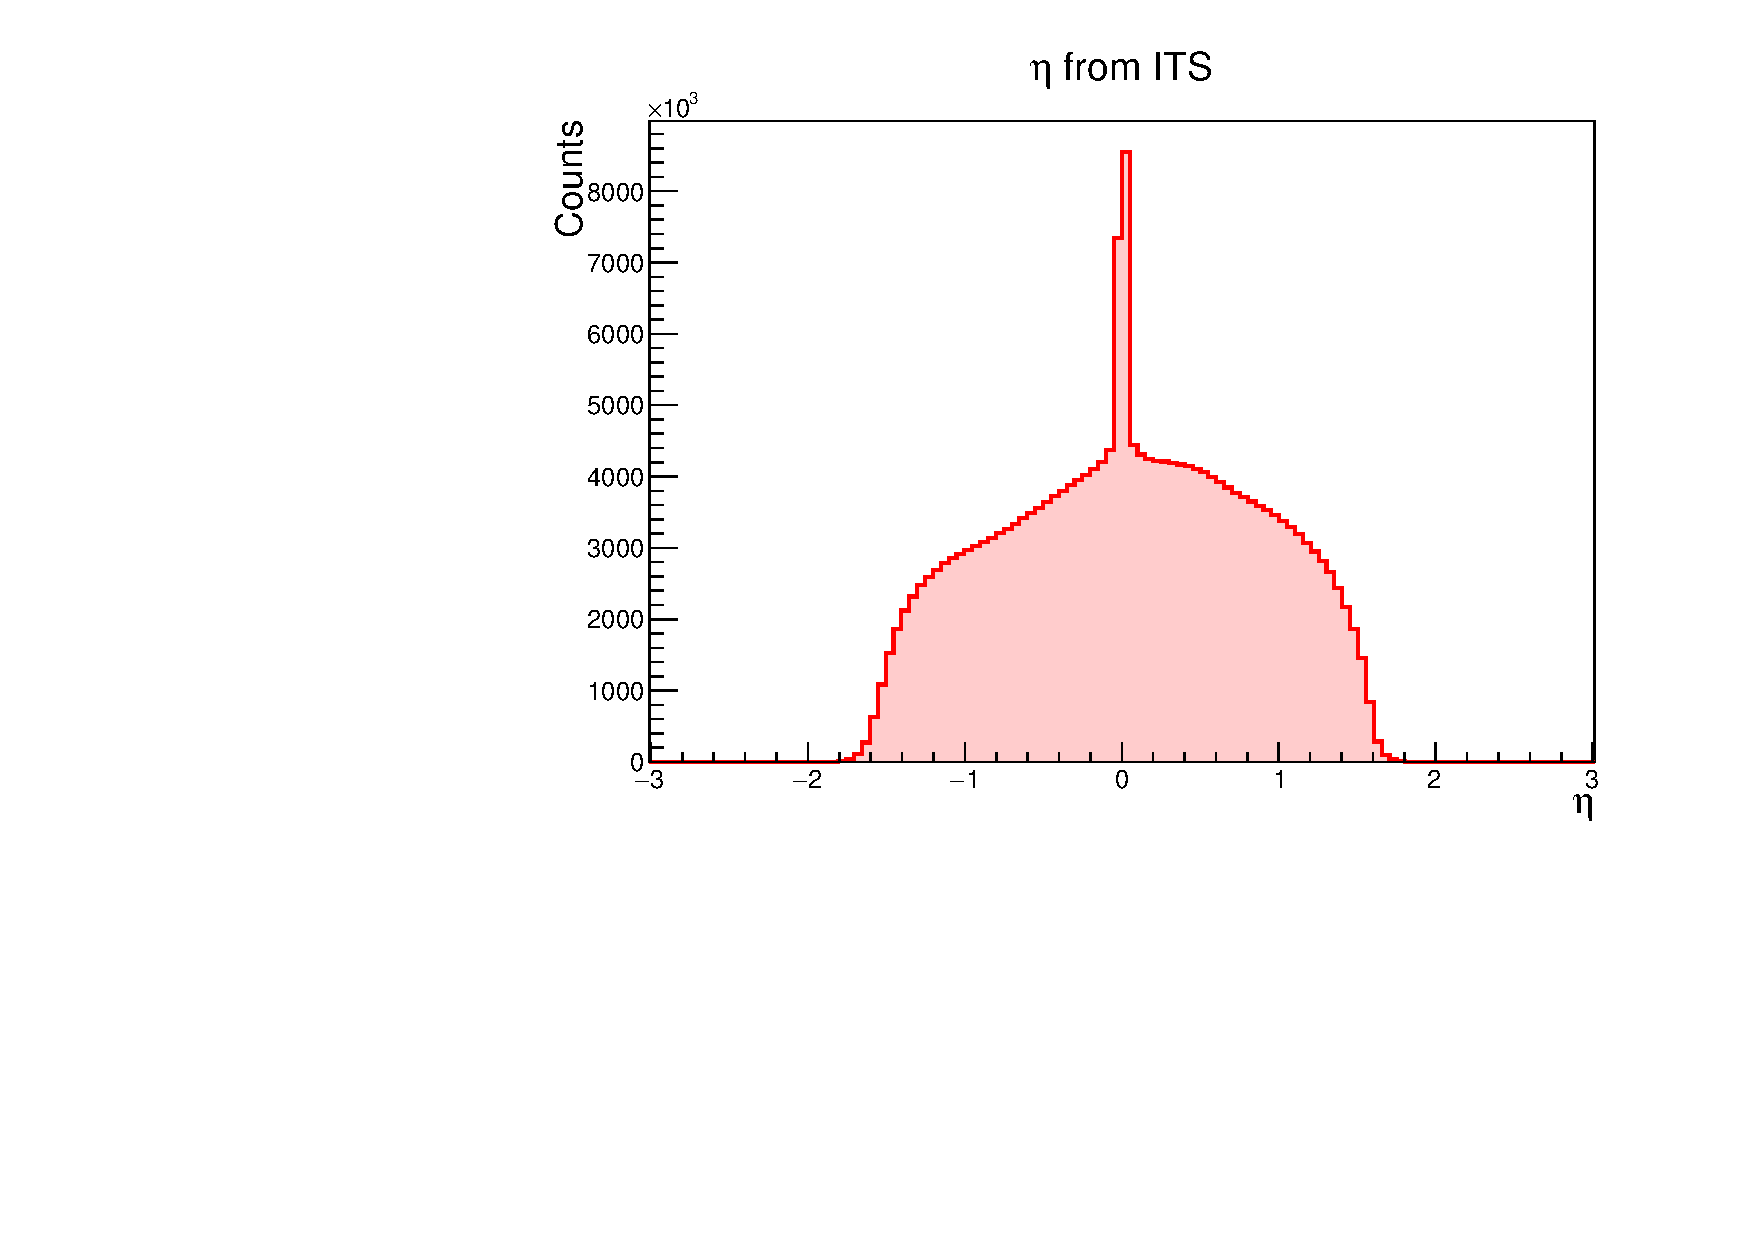
\includegraphics[width=\linewidth]{Plots/pass4_TracksIU_nohasITS/eta.pdf}
        \caption{Histogram of $\eta$ for tracks detected in the central barrel. Note the lopsided distribution and large spike at the centre.}
        \label{fig:nohasITS_eta}
    \end{subfigure}
    \hfill
    \begin{subfigure}[t]{.49\linewidth}
        \centering
        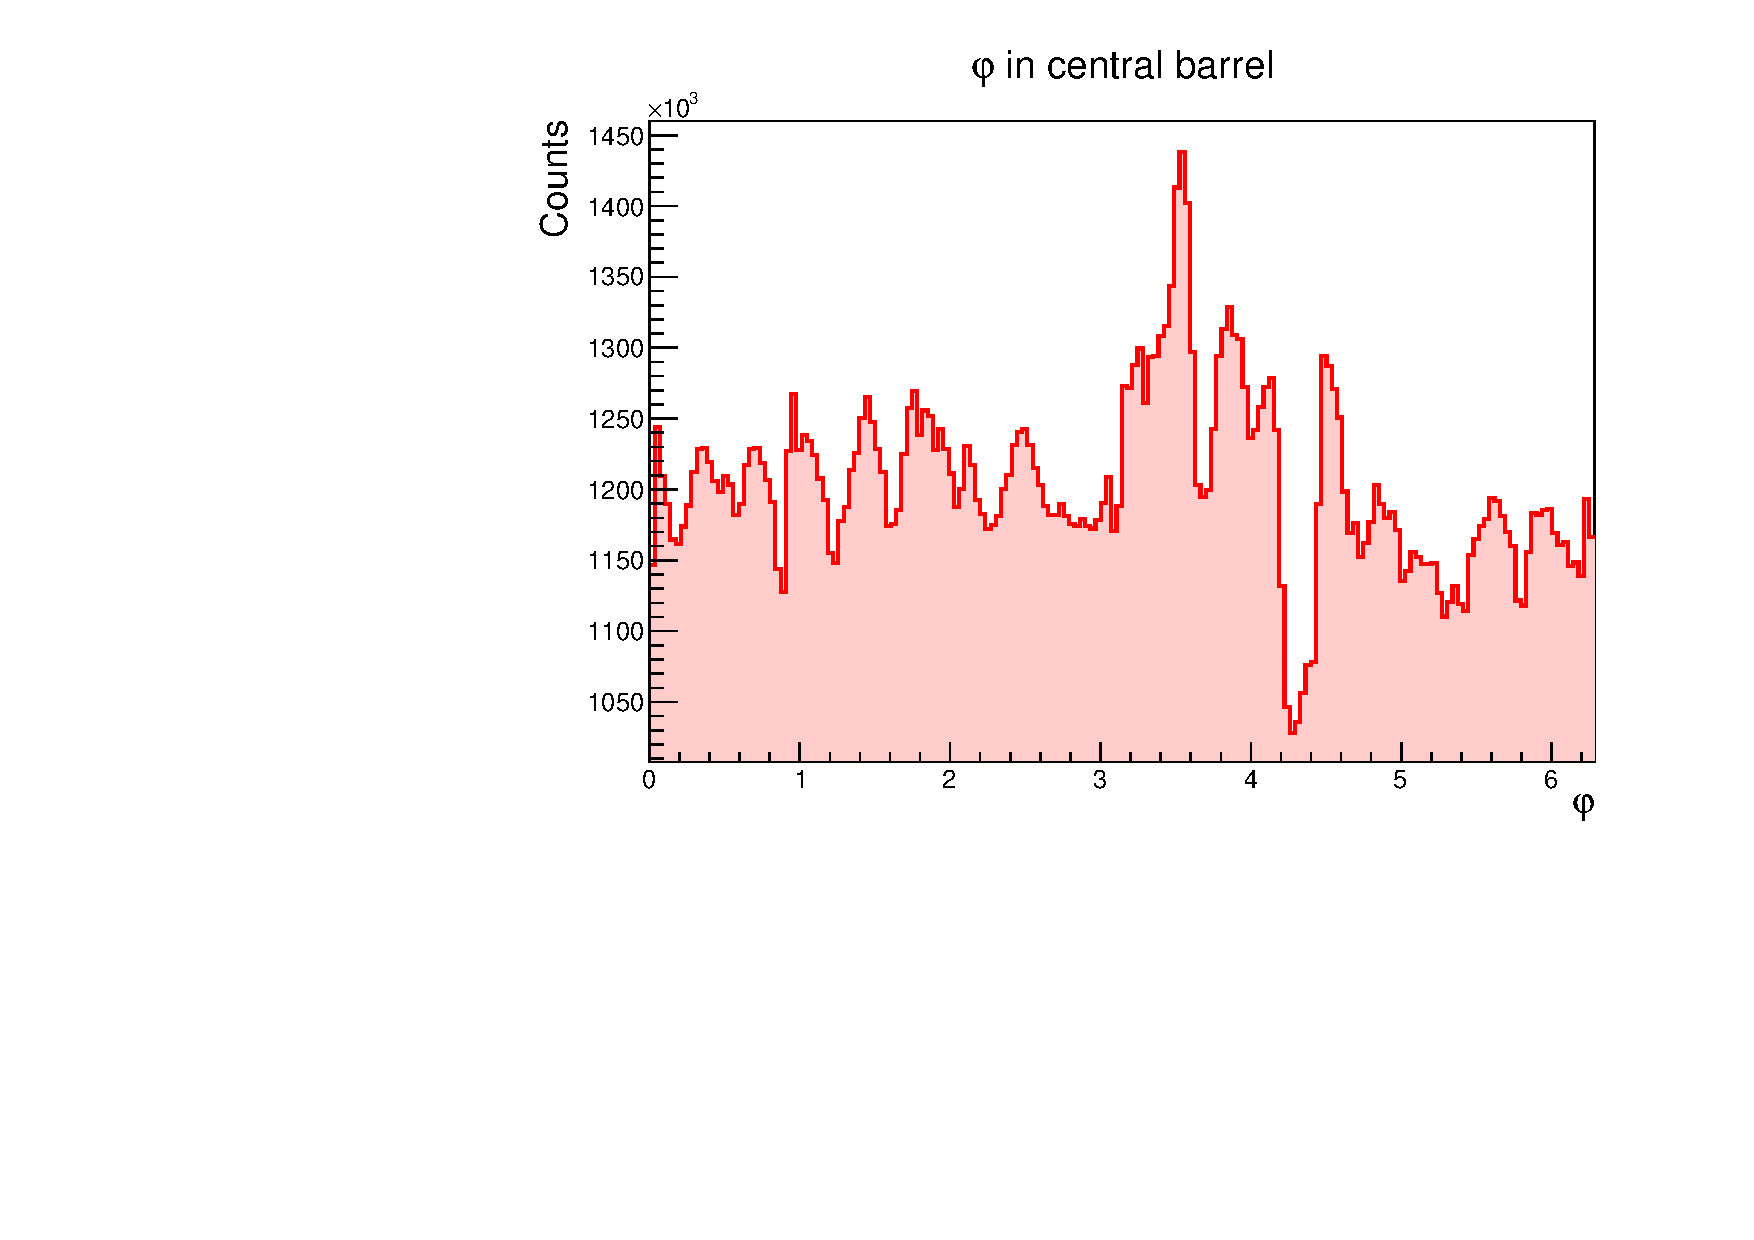
\includegraphics[width=\linewidth]{Plots/pass4_TracksIU_nohasITS/phi.pdf}
        \caption{Histogram of $\varphi$ for tracks detected in the central barrel.}
        \label{fig:nohasITS_phi}
    \end{subfigure}
    \begin{subfigure}[t]{.49\linewidth}
        \centering
        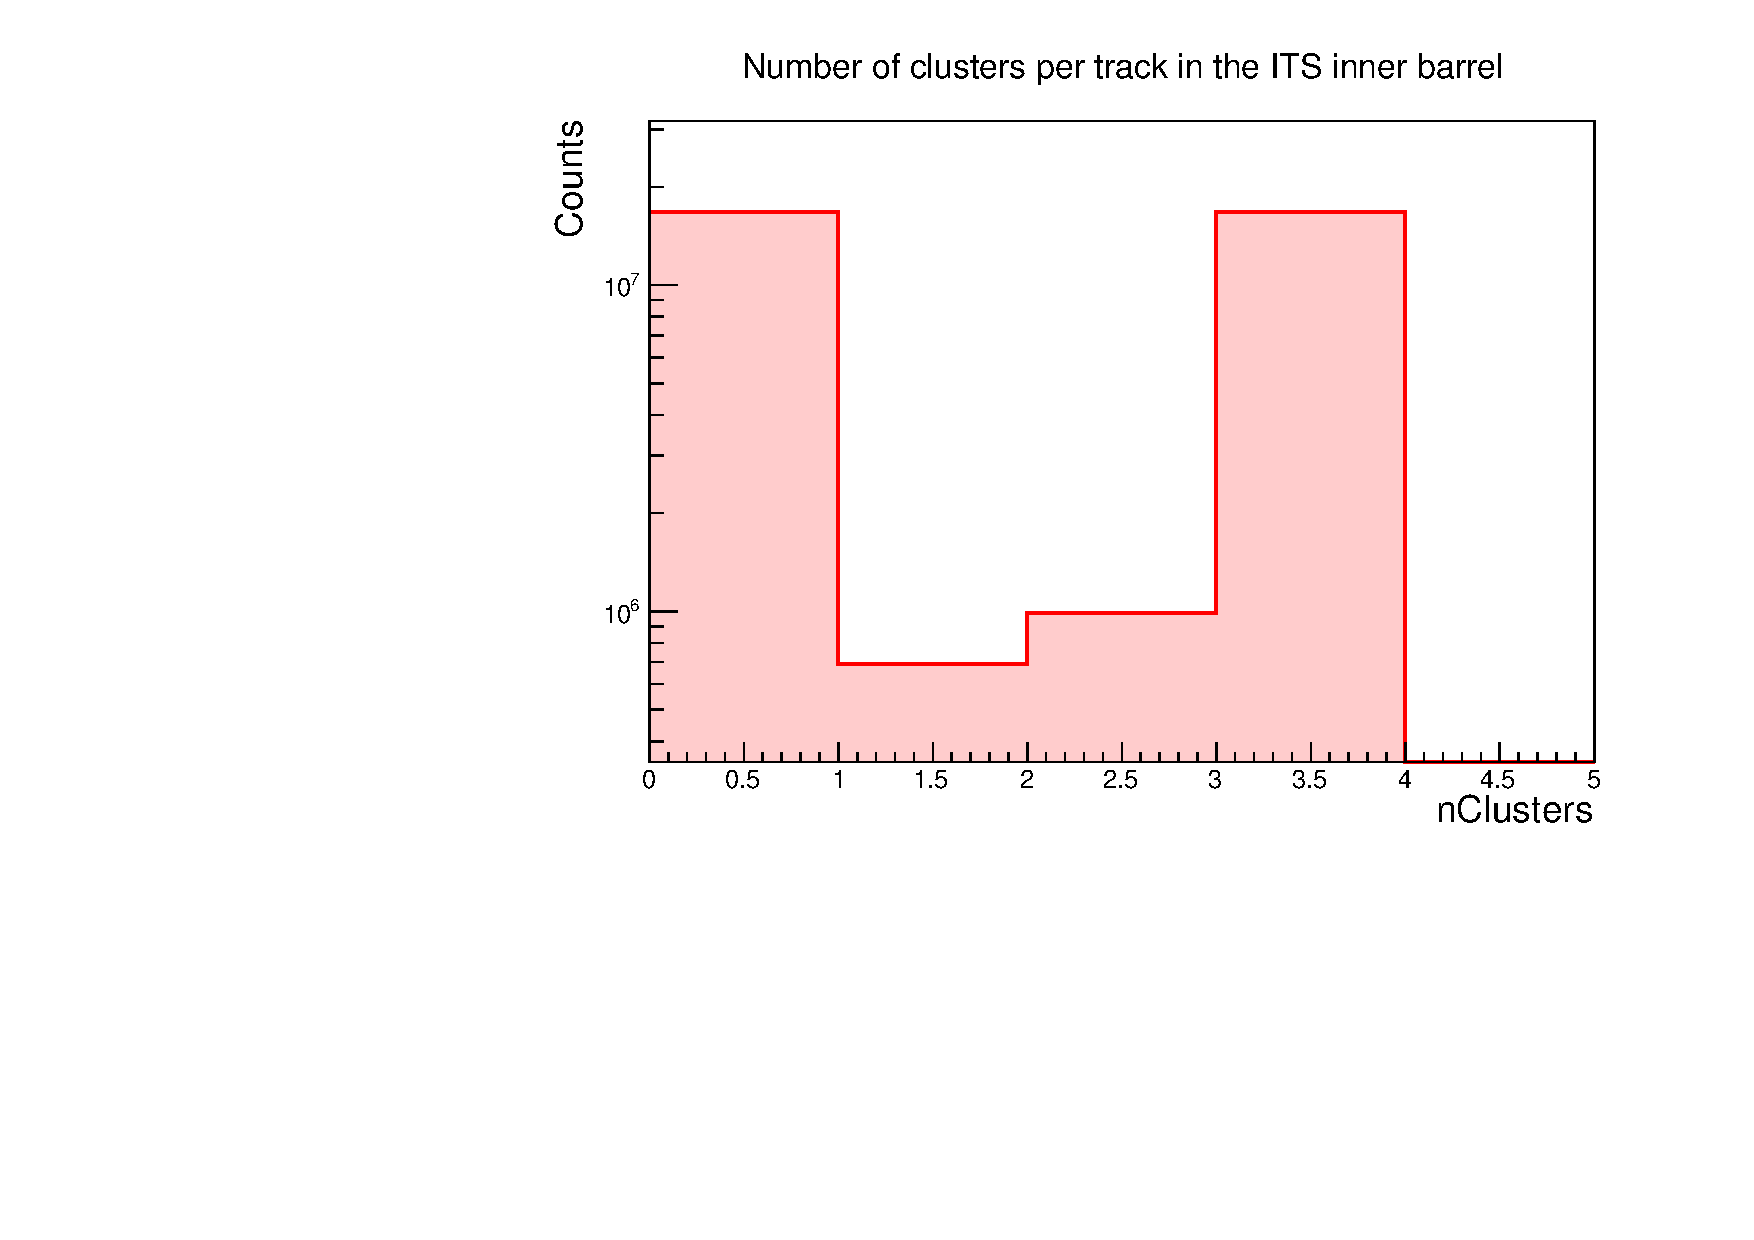
\includegraphics[width=\linewidth]{Plots/pass4_TracksIU_nohasITS/itsNClsInnerBarrel.pdf}
        \caption{Histogram of the number of clusters in the ITS inner barrel that contribute to a given track. Note here the relatively large number of tracks with 0 clusters in the inner barrel.}
        \label{fig:nohasITS_NCls_InnerBarrel}
    \end{subfigure}
    \hfill 
    \begin{subfigure}[t]{.49\linewidth}
        \centering
        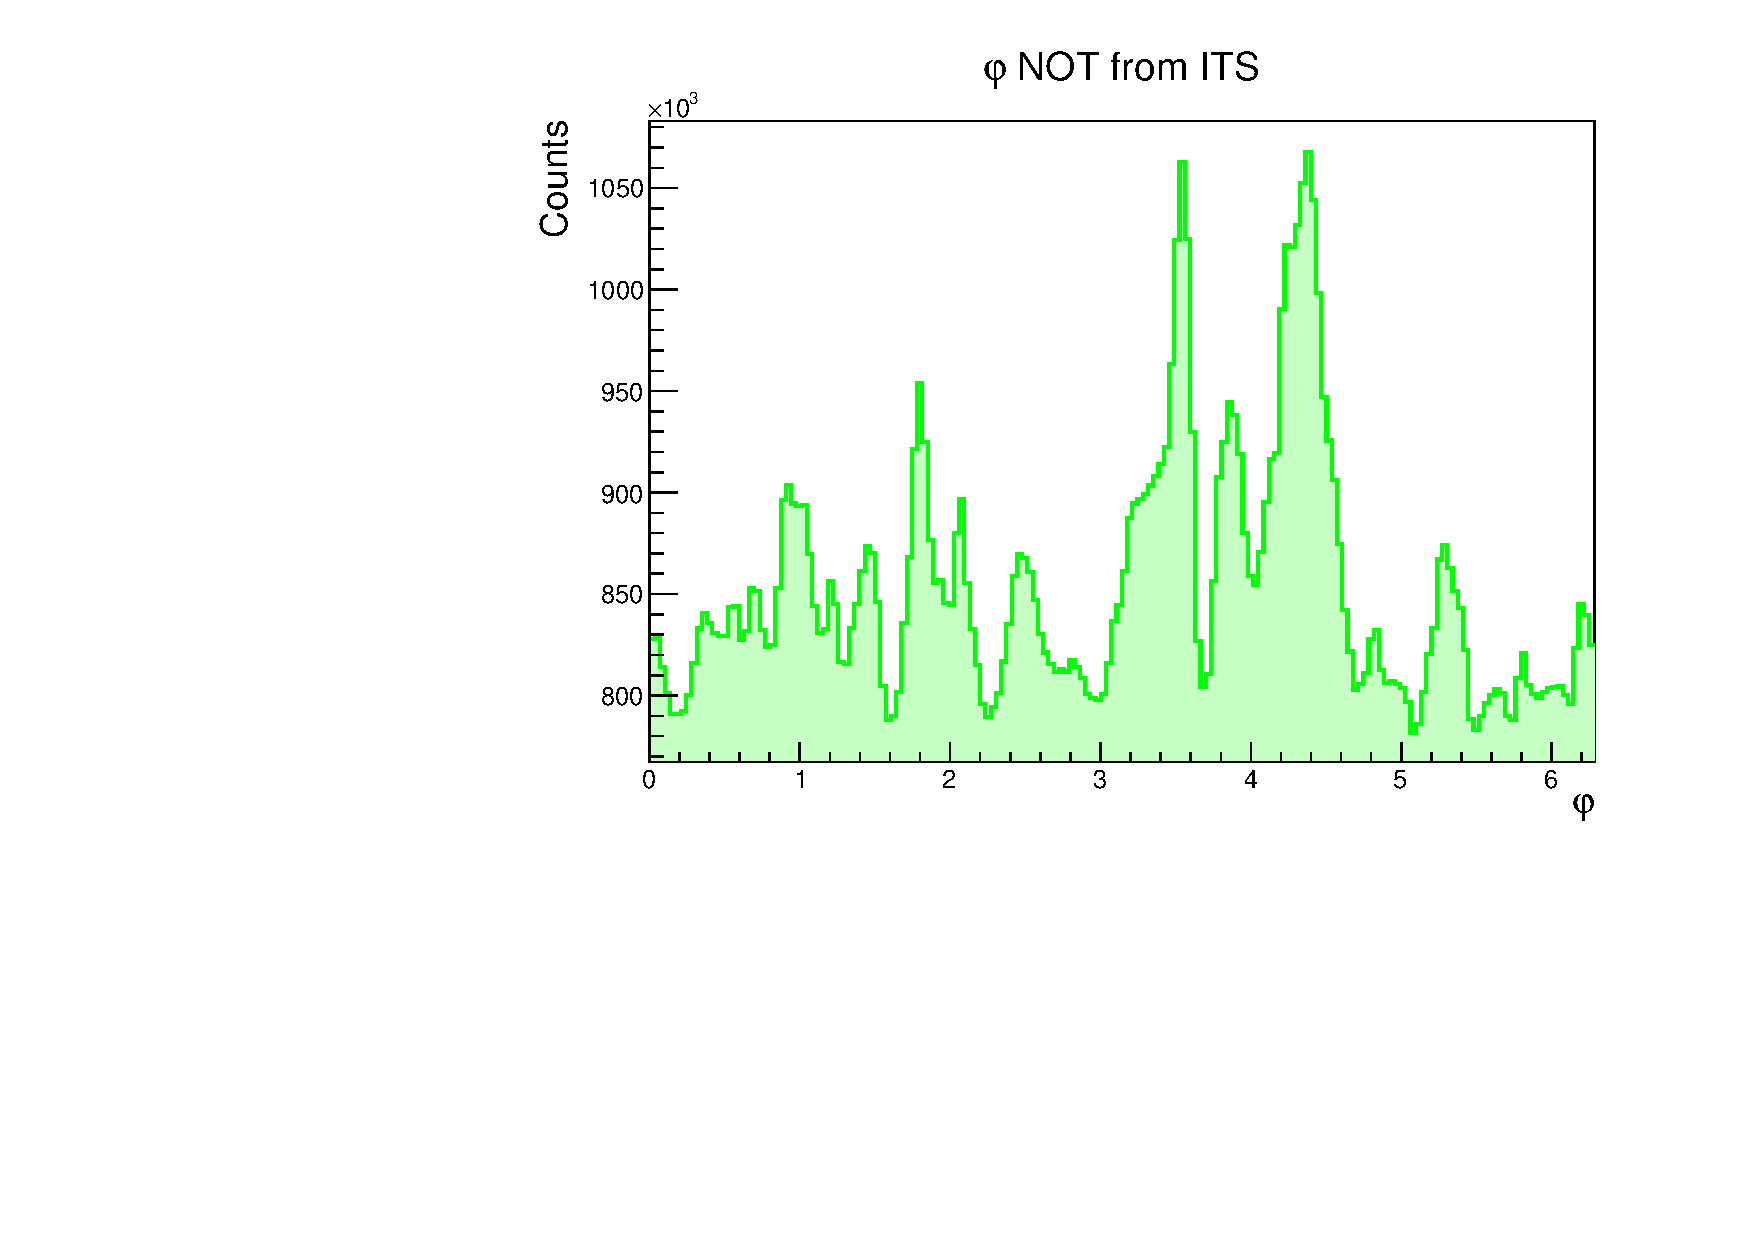
\includegraphics[width=\linewidth]{Plots/phi_no_ITS.pdf}
        \caption{Histogram of $\varphi$ for tracks detected in the barrel but specifically those that were not detected in the ITS.}
        \label{fig:nohasITS_phi_no_ITS}
    \end{subfigure}
\caption[Histograms of $\eta$, $\varphi$, and ITS inner barrel \OldTexttt{nClusters} for tracks in the central barrel]{Some histograms of kinematic variables of tracks detected in the central barrel. This is data for the tracks at their innermost update, but that does not necessarily mean the tracks are only from the ITS. Uniform and symmetric distributions (aside from the number of clusters) are expected but not seen.}
\label{fig:ITS_1D_nohasITS}
\end{figure}

Upon seeing the ITS tracks, a few questions arise. Firstly, we see how the $\eta$ distribution is remarkably uniform and symmetric, especially considering the form of \cref{fig:nohasITS_eta}. However, there is clearly a dip in the middle, which contradicts our reasoning for the lopsided distribution in the MFT as we would expect a distribution peaked at the centre and slowly decreasing as it goes outwards. This might be explained by the number of tracks at that pseudorapidity being so large that pile-up or overloading occurs, leading to missed tracks. \Cref{fig:nohasITS_eta} supports our expectations as it is sharply peaked at the centre. This is requires more investigation alongside the read-out architecture.

\begin{figure}[H]%
    \centering
    \begin{subfigure}[t]{.49\linewidth}
        \centering
        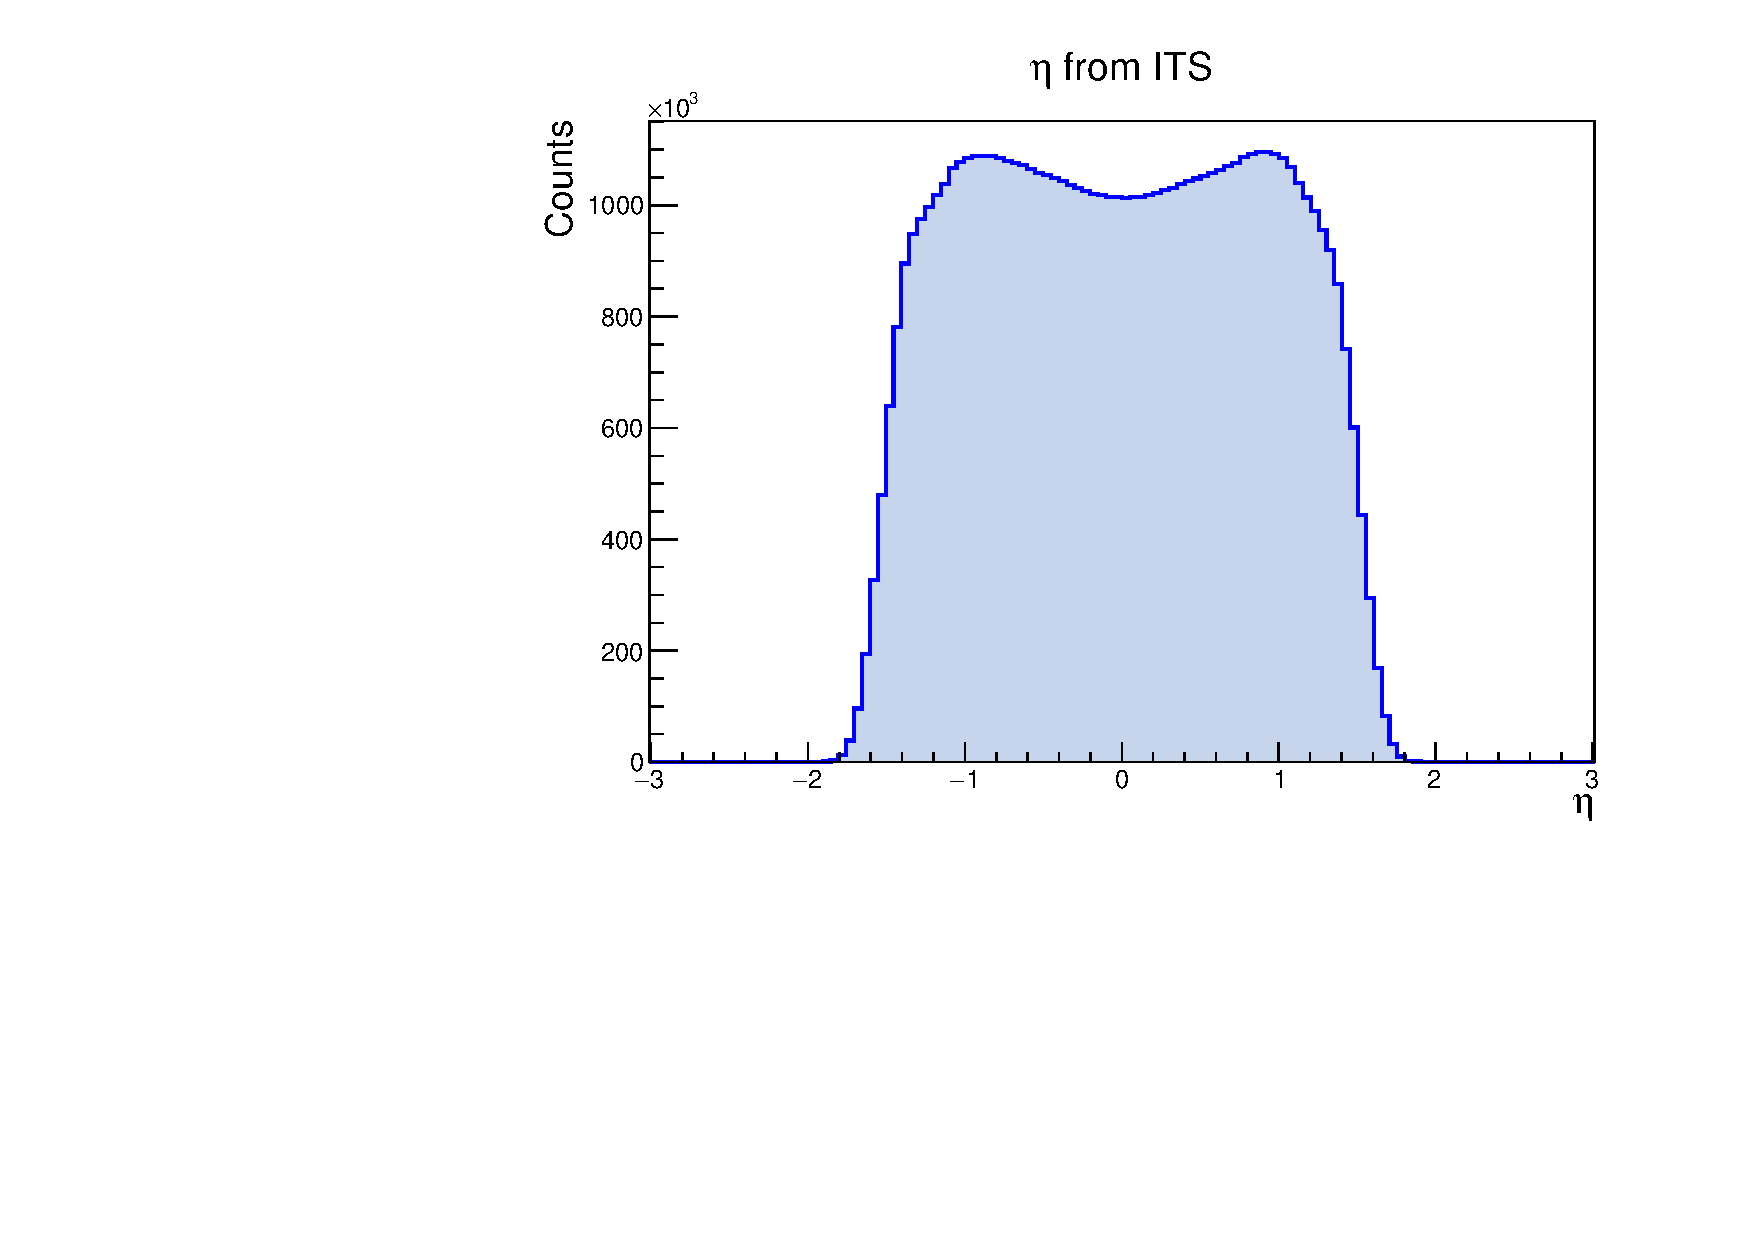
\includegraphics[width=\linewidth]{Plots/pass4_TracksIU/eta.pdf}
        \caption{Histogram of $\eta$ for tracks detected in the ITS. Note the uniform and symmetric distribution, but with a valley in the centre.}
        \label{fig:ITS_eta}
    \end{subfigure}
    \hfill
    \begin{subfigure}[t]{.49\linewidth}
        \centering
        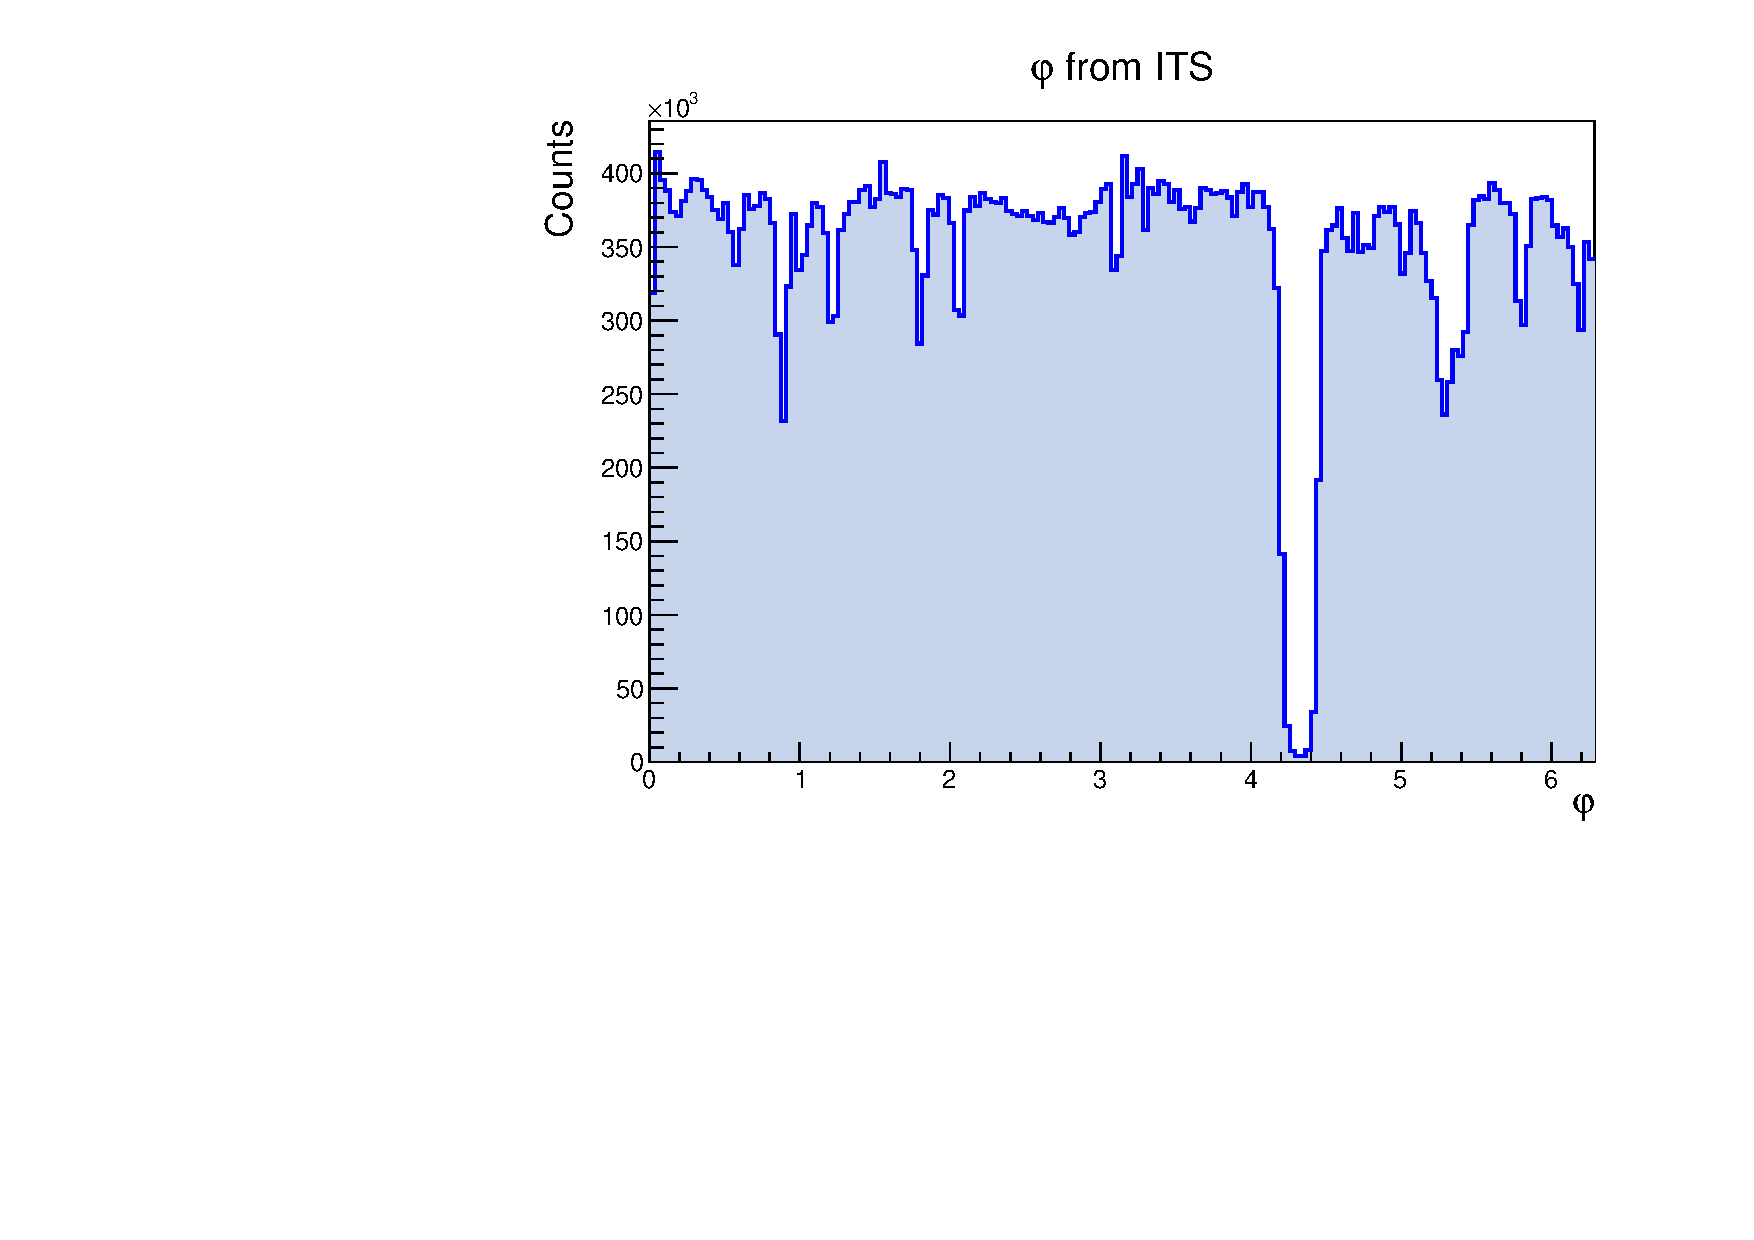
\includegraphics[width=\linewidth]{Plots/pass4_TracksIU/phi.pdf}
        \caption{Histogram of $\varphi$ for tracks detected in the ITS. Note how the distribution is overall much more uniform, but with a large valley around 4.3.}
        \label{fig:ITS_phi}
    \end{subfigure}
    \begin{subfigure}[t]{.49\linewidth}
        \centering
        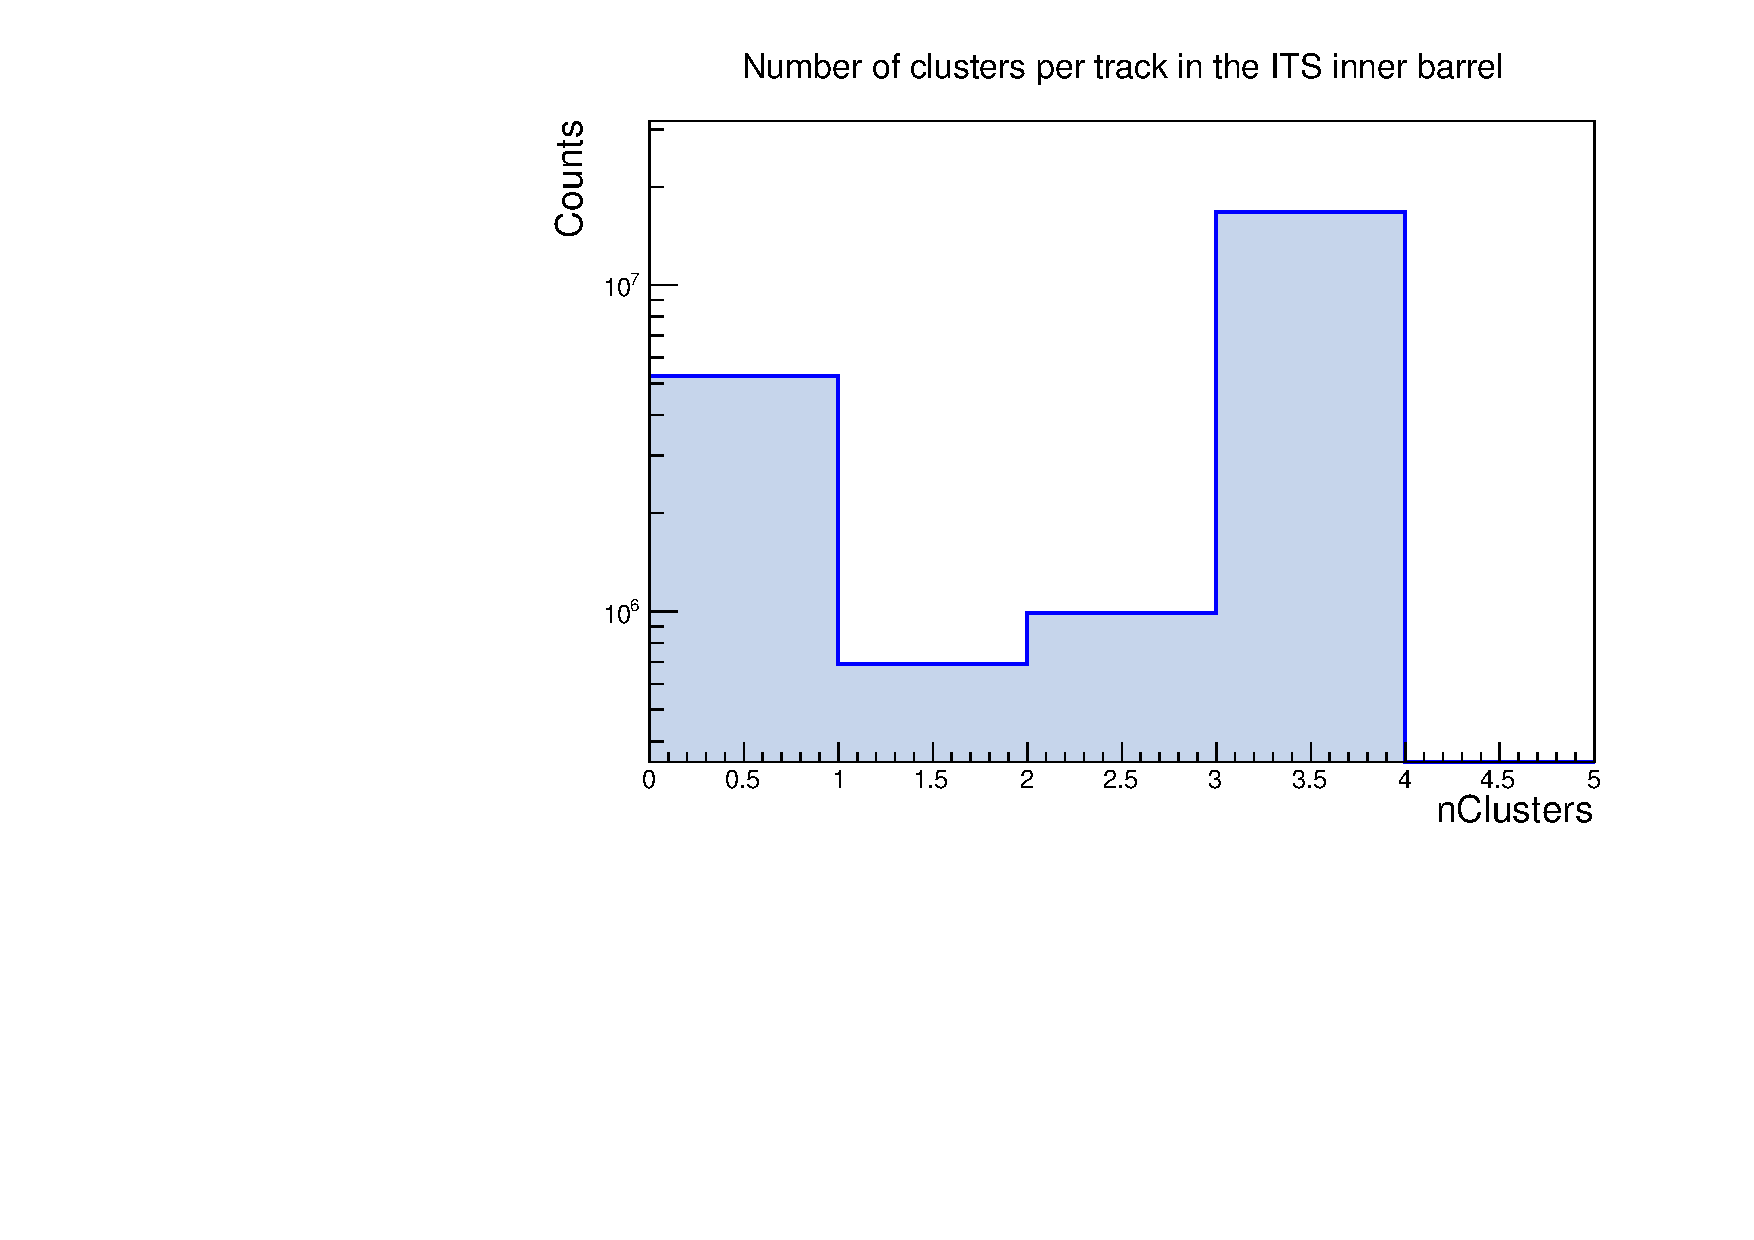
\includegraphics[width=\linewidth]{Plots/pass4_TracksIU/itsNClsInnerBarrel.pdf}
        \caption{Histogram of number of clusters in the ITS inner barrel that contribute to a given track. The number of tracks with 0 clusters is far fewer than in \cref{fig:nohasITS_NCls_InnerBarrel}}
        \label{fig:ITS_NCls_InnerBarrel}
    \end{subfigure}
    \hfill
    \begin{subfigure}[t]{.49\linewidth}
        \centering
        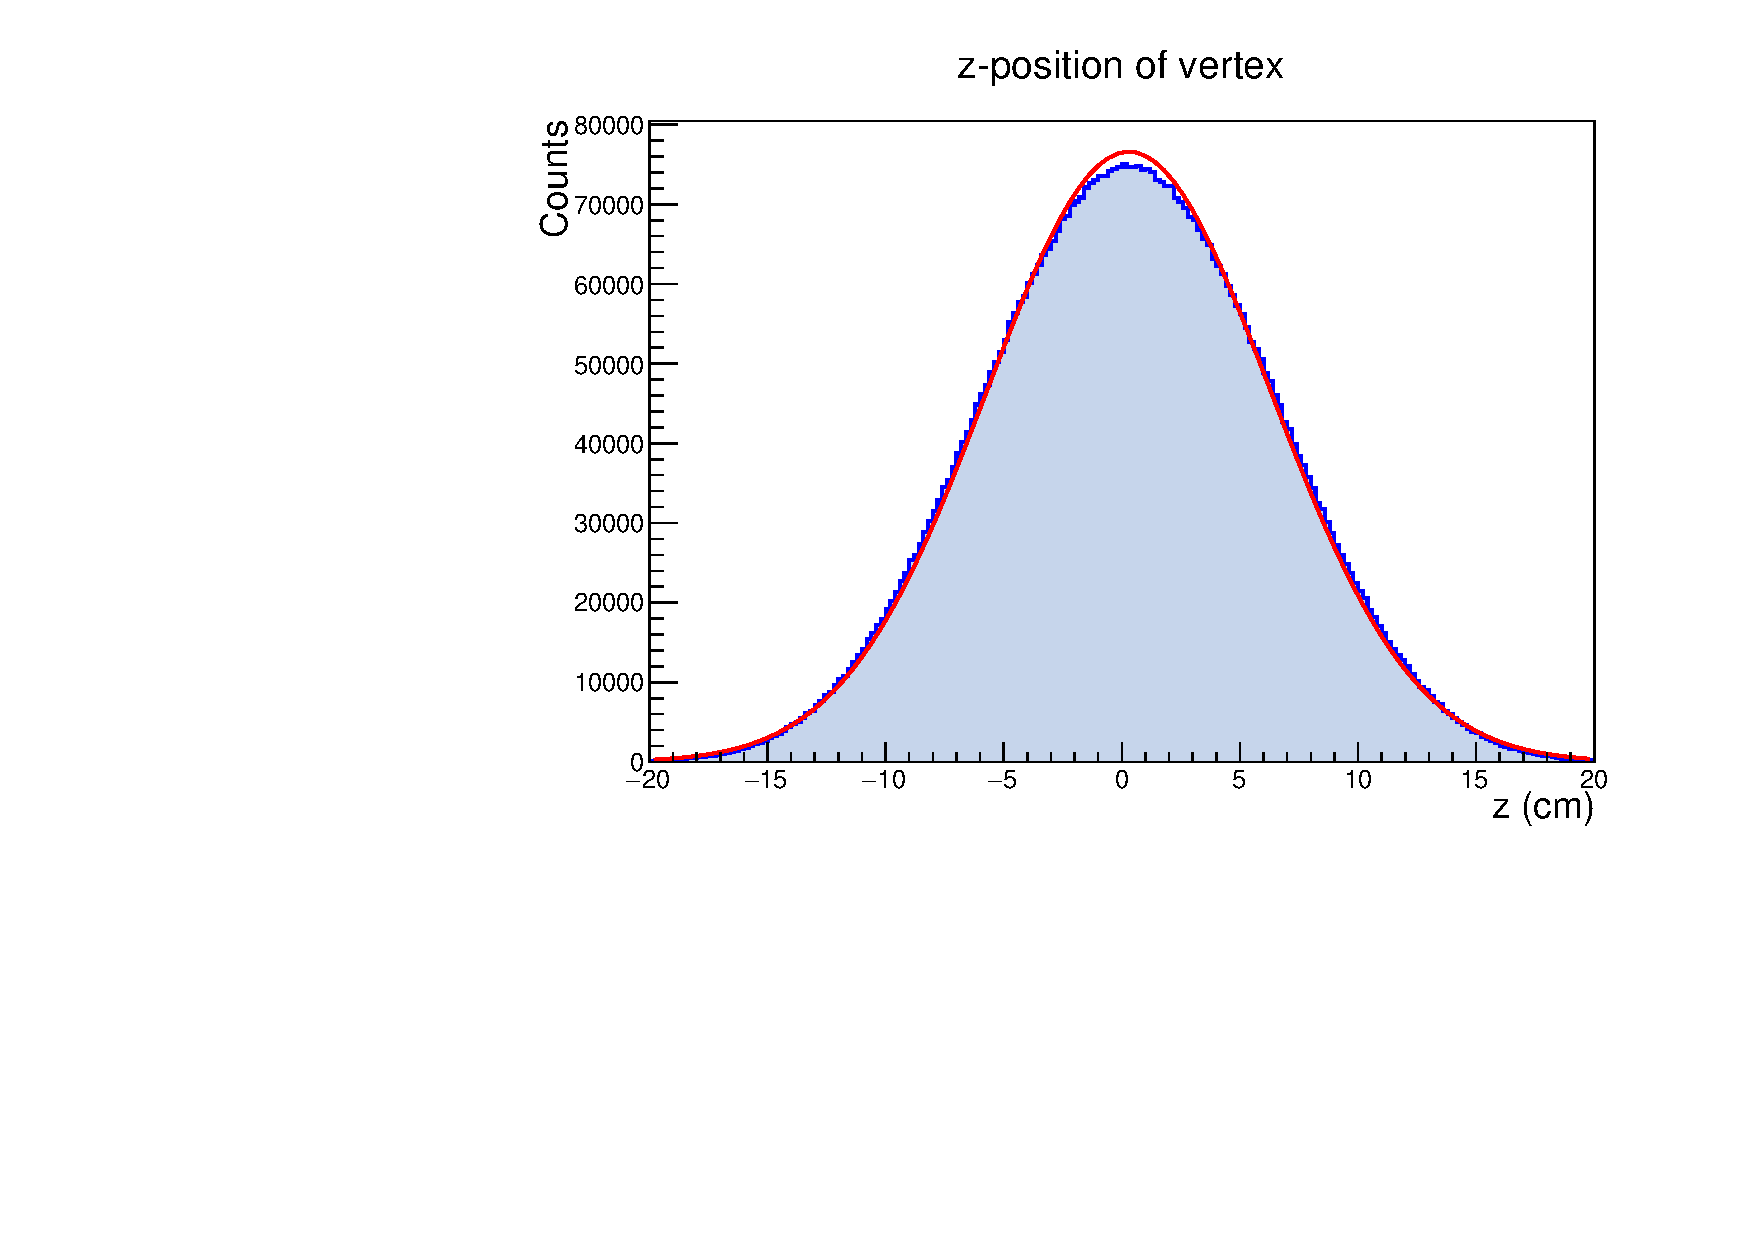
\includegraphics[width=\linewidth]{Plots/pass4_TracksIU/Z.pdf}
        \caption{Histogram of the $z$-position of the collision vertex. A gaussian function is fit to the data, with $\mu=0.2951$, $\sigma=6.0205$. Note that this is not the position as determined by the ITS alone as that information is not in the data model at present. Each entry is a collision, not a track.}
        \label{fig:ITS_Z}
    \end{subfigure}
\caption[Histograms of $\eta$, $\varphi$, \OldTexttt{nClusters}, and $z$ for tracks in the ITS]{Histograms of kinematic variables of tracks detected by the ITS as well as of collisions.}
\label{fig:ITS_1D}
\end{figure}

The $\varphi$ distribution in \cref{fig:ITS_phi} looks much more uniform, at least on the whole, than in \cref{fig:nohasITS_phi}. This is made more obvious when taking \cref{fig:nohasITS_phi_no_ITS} into account as there appears to be no pattern or symmetry in the $\varphi$ distribution of tracks when not detected in the ITS. No reason for this is apparent to us so this requires a more in-depth investigation. The valley in \cref{fig:ITS_phi} at about 4.3, and smaller ones in other places, is certainly a concern. \Cref{fig:ITS_eta_phi} helps to elucidate the situation as we can see there is no $\eta$ dependence on the large gap, so we are inclined to say that a whole strip of detectors in the ITS, running along the $z$-axis, was not functioning properly. This is reasonable as the electronics in the ITS group pixel chips together in that direction. Other smaller gaps can also be seen, spanning short ranges of $\eta$, which would imply short strips of pixel chips weren't working properly.

\begin{figure}[h]
    \begin{center}
        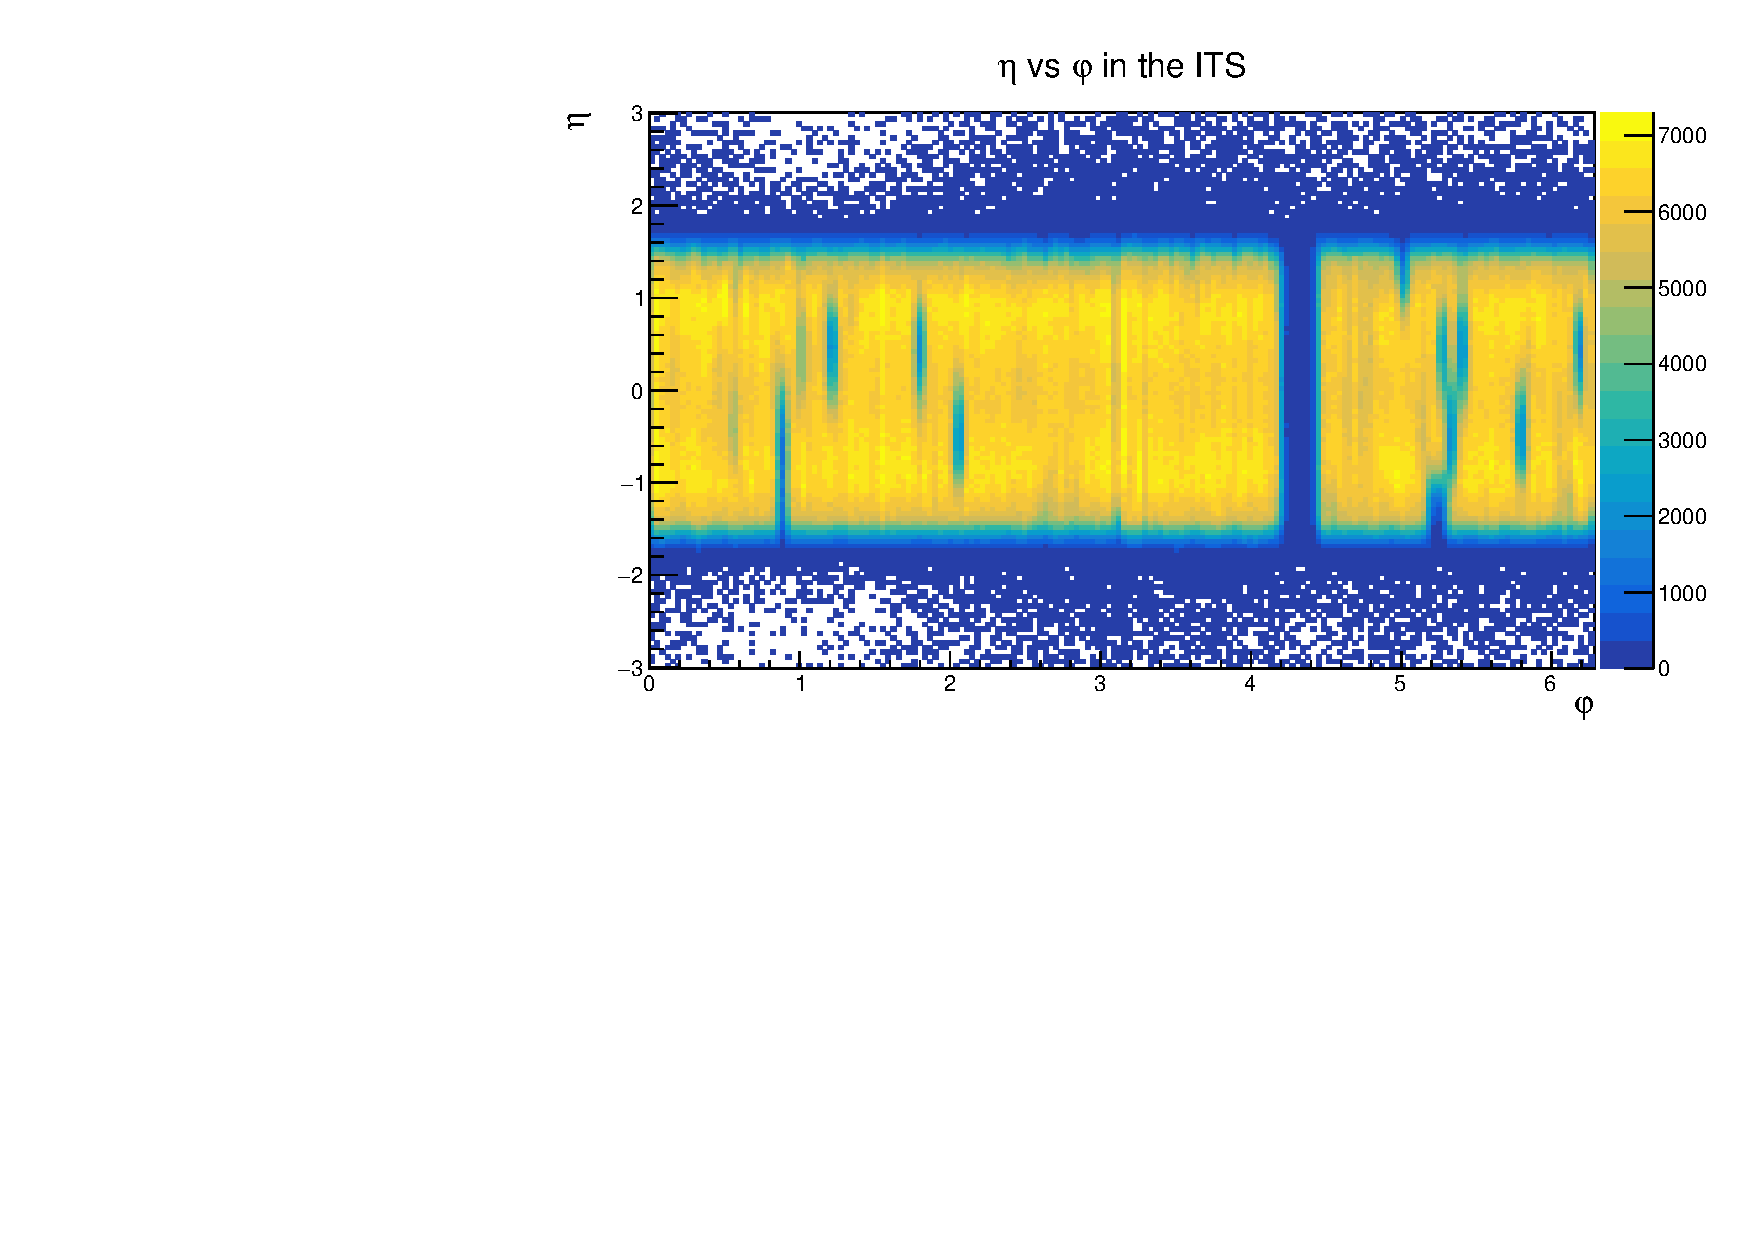
\includegraphics[width=.8\textwidth]{Plots/pass4_TracksIU/eta_phi.pdf}
        \caption[$\eta$-$\varphi$ histogram for tracks in the ITS]{Histogram of $\eta$ and $\varphi$ for tracks detected in the ITS. The valley at $\varphi\approx 4.3$ can clearly be seen, with no specific $\eta$ region being affected. Note a few other smaller strips of lower counts.}
        \label{fig:ITS_eta_phi}
    \end{center}
\end{figure}

Looking at \cref{fig:ITS_NCls_InnerBarrel} in comparison to \cref{fig:nohasITS_NCls_InnerBarrel}, we see a decrease in the number of tracks with no clusters in the inner barrel. This is clearly as expected. Lastly, the $z$-position of the collision vertex is shown in \cref{fig:ITS_Z} with a gaussian function fit to it. Important to note here is that each entry in the histogram is not a track, as it has been before, but rather a collision in the \texttt{aod::Collisions} table. While the ITS is the main detector that determines the vertex position, there is little information about what information was used to determine the vertex so little can be said about how the ITS performs in this regard. Nevertheless, this is a useful plot to look at to make sure that collisions are happening both as close to the IP as possible but also symmetrically around the IP. Both these conditions are met in this case, within acceptable tolerance. 

\bigskip

The last histograms to interrogate are ones corresponding to the clusters contributing to tracks in the ITS, shown in \cref{fig:ITS_Clusters}. The left is easy to interpret, showing the number of ITS clusters used in each track. Interestingly it appears to have a minimum of 4 clusters per track. If these tracks are from the TPC regime, this doesn't make sense, but if they are standalone tracks then we may have discovered something about the method used.

\begin{figure}[h]%
    \centering
    \begin{subfigure}[t]{.49\linewidth}
        \centering
        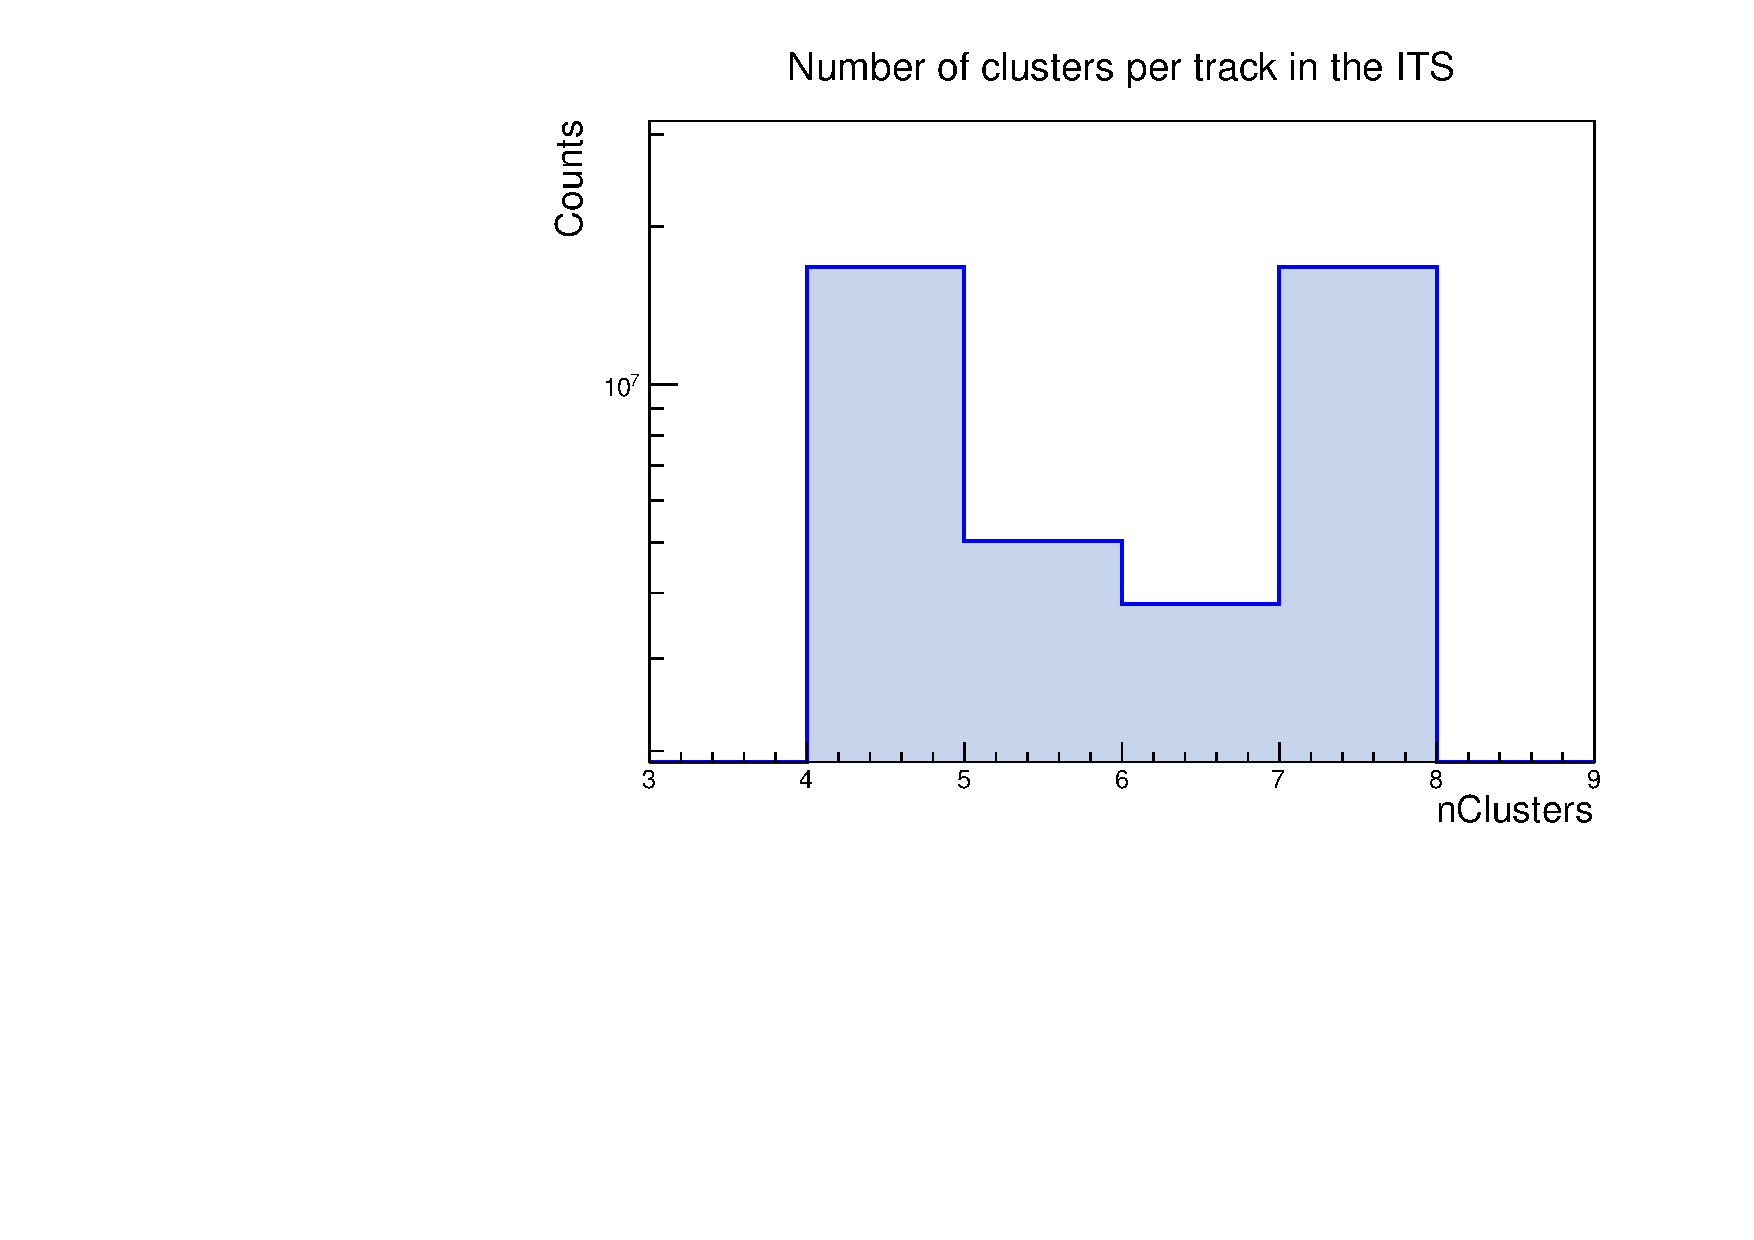
\includegraphics[width=\linewidth]{Plots/pass4_TracksIU/itsNCls.pdf}
        \caption{Histogram of number of clusters in the entire ITS that contribute to a given track. Note the cut-off at 4, seeming to imply a minimum number of clusters per track.}
        \label{fig:ITS_NCls}
    \end{subfigure}
    \hfill
    \begin{subfigure}[t]{.49\linewidth}
        \centering
        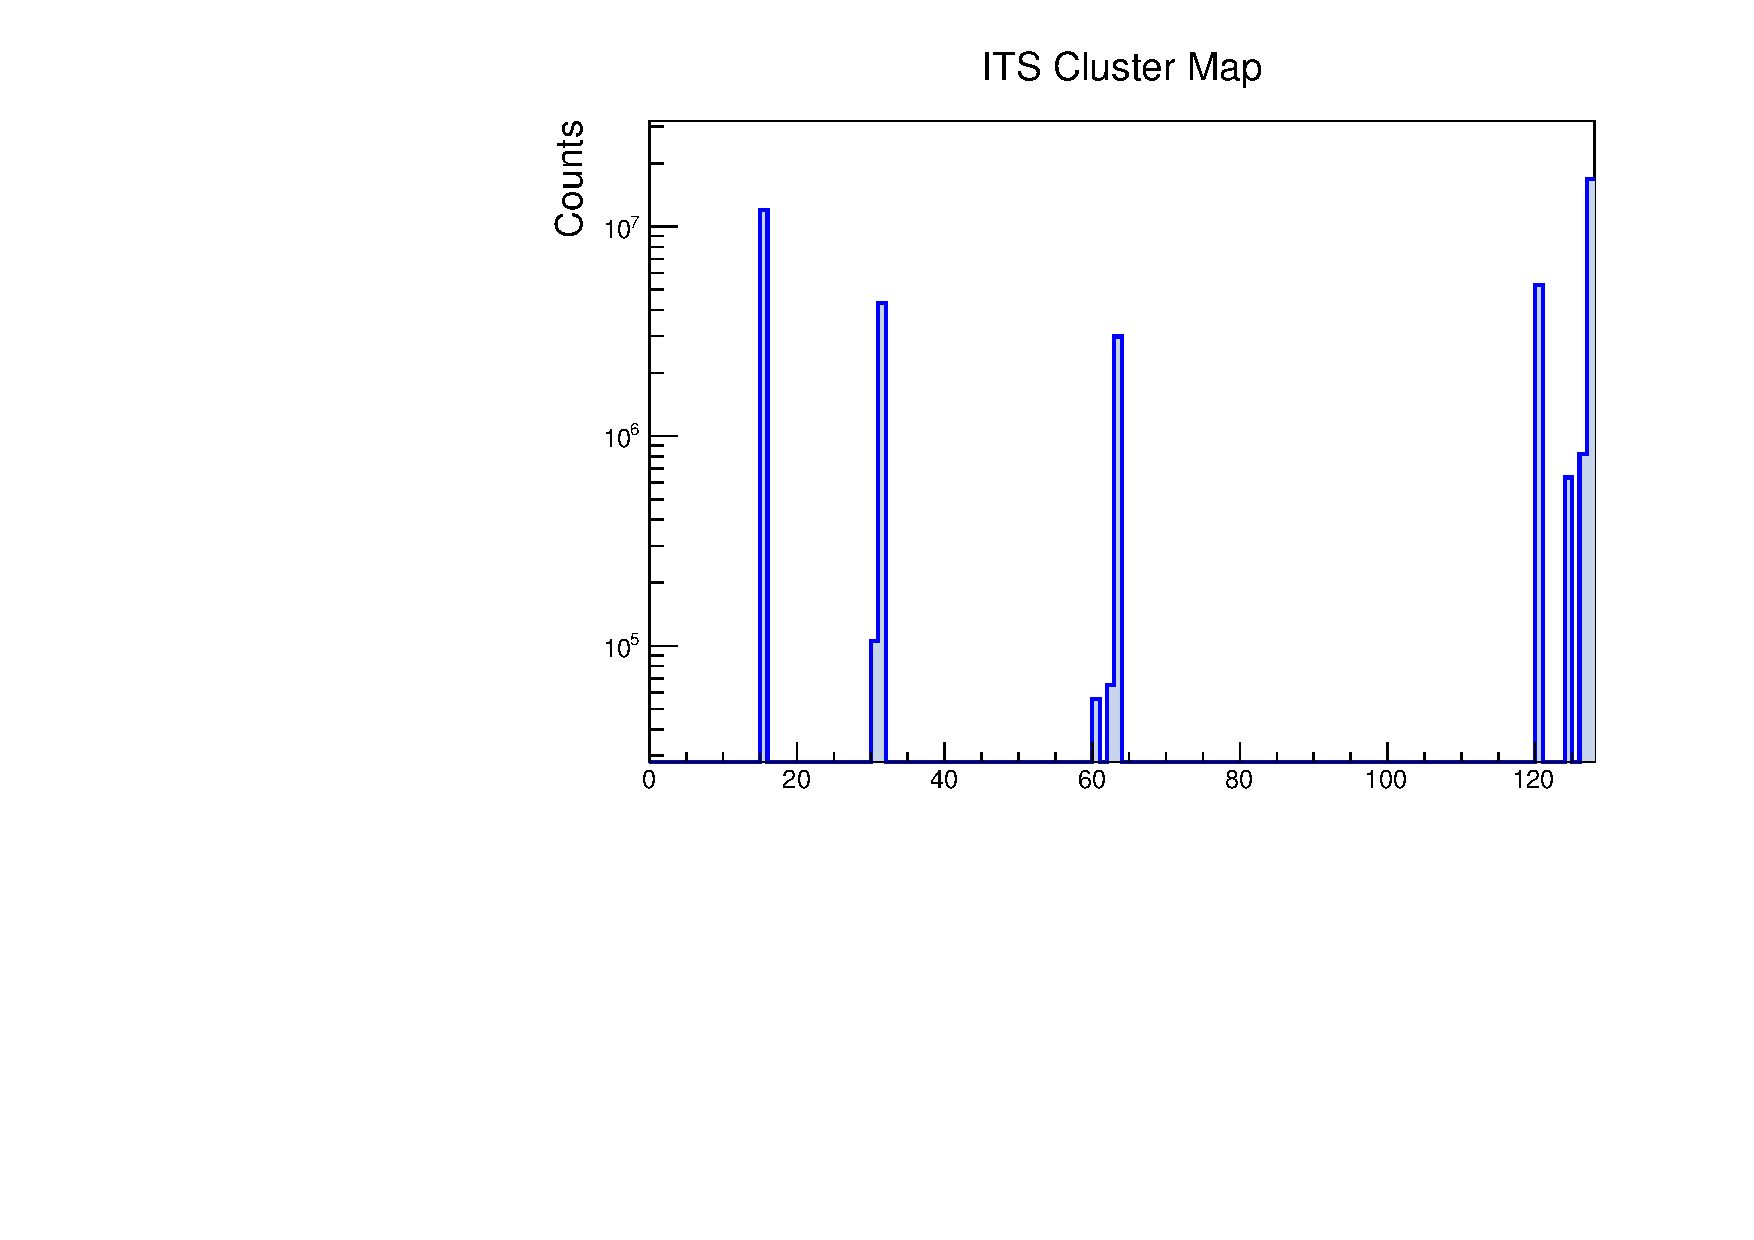
\includegraphics[width=\linewidth]{Plots/pass4_TracksIU/itsClusterMap.pdf}
        \caption{Histogram of the so-called ``Cluster Map'' of the ITS, where each layer in the ITS is assigned a bit, starting from the innermost.}
        \label{fig:ITS_ClusterMap}
    \end{subfigure}
\caption[Histograms of cluster information for tracks in the ITS]{Additional histograms with information about the ITS clusters used in track finding.}
\label{fig:ITS_Clusters}
\end{figure}

On the right of \cref{fig:ITS_Clusters} is the ``Cluster Map'' of the ITS. The column in the data model contains an 8 bit unsigned integer with each bit assigned to a layer, excluding the last bit. If a track has a cluster in a specific layer, the bit is set to 1, otherwise it is set to 0. Since integers have unique representations in binary, we can see exactly which layers contributed to a given track simply by decoding the integer. As seen in \cref{fig:ITS_ClusterMap}, the lowest is 15 meaning the innermost 4 layers had clusters contributing, and the highest is 127 meaning all layers had clusters contributing. In between those is all combinations of the 7 bits, but only those with 4 or more clusters, as expected from \cref{fig:ITS_NCls}. 

\section{Discussion and Recommendations}\label{sec:DiscussionRecommendations}
Our methods of analysis for the most part came down to interpreting histograms of kinematic variables through the lens of assumed isotropic emission of particles. The shape of the coordinate system and detector geometry had to be considered in order to explain some things and there was a lot of guesswork as to the configuration of the detectors and reconstruction process/analysis framework. In this section we present some improvements that can be made to this process.

There were many times during our analysis where we came up against a limitation in the analysis software that restricted our ability to see the details we were after. This really comes down to the fact that the types of analysis that O2 was (and still is being) built for are not the type that we were looking to do. Given more time to attain a greater understanding of the inner workings of particularly the steps from CTFs to AODs, we might have been able to delve into the belly of the beast and find the data ourselves. Since we were limited by our time this year, the best we can do is recommend some modifications to the AOD data model that would lend themselves to these analyses. 

We recommend introducing more detail about the tracks in the MFT, such as the position of hits in each disk, or even a simple ``Cluster Map''-style column in the \texttt{aod::MFTTracks} table to be able to see which disks or detector planes contributed to the track. At time of writing, there is no way to view the vertex position data as determined by the ITS or the MFT alone. Adding this capability would allow for an investigation into the improvement of the new ITS and MFT in that sector, which we were unable to do.

Outside the realm of modifying O2 and the data model, there is more that could be done to properly verify if the distributions we see for, say $\eta$ and $\varphi$, are correct. We have attempted to explain them from a physical motivation but comparison to simulated data would prove the most robust way to check that there are no large systematic errors. In the interest of determining how the MFT has improved the tracking capabilities in the forward region, the old techniques used in Runs 1 and 2 using the MCH could be implemented on new data and compared to the new technique on the same data. This would require investigation of the analysis framework at a much more involved level than was possible in this report but could lead to some interesting results. Once again simulation could aid in this endeavour. 

Lastly, we were left with many questions about the details of the track reconstruction, read-out architecture, and columns in the data model such as the $z$ variable in \texttt{aod::MFTTracks}. This effectively comes down to the documentation surrounding these detectors and analysis framework, so a concerted effort to improve that documentation would be greatly appreciated by people new to the ALICE group and to these detectors. 

\section{Conclusion}\label{sec:Conclusion}
The advent of Run 3 at the LHC, with its increased energy and luminosity, brought a number of new challenges that required the ALICE detectors and analysis framework to be upgraded. Among the detector upgrades were two new silicon tracking detectors; the ITS and MFT. In this report we used the new O2 analysis framework to look at distributions of variables relating to particle tracks in either the ITS or MFT, using pilot beam data from October 2021. The intention was both to learn the new framework and to determine if the new detectors are performing as expected.

Before any analysis could be done, the new framework had to be learned. Due to its need to be efficient and lightweight on hard disk and memory usage, it is very particular about how things must be structured. Learning O2 took up the majority of the time spent on this project and the basics are presented in \cref{sec:AnalysingWithO2}. 

Simulation of data for comparison was outside the scope of this project so the notion of an ``expected performance'' had to come from an understanding of the physical design of the detectors as well as an interpretation of the read-out architecture and track reconstruction process as outlined in the Technical Design Reports of the two detectors. Isotropic emission of particles from the IP was assumed which led to expectations of smooth, if not uniform, distributions in most cases. Where this was not seen and the geometry of the sensitive material of the detectors couldn't explain the discrepancy, specific areas of research into the detectors were recommended. This analysis is presented in \cref{sec:OurAnalysis}.

Due to time limitations, this report could only give a qualitative review of the performance of the new detectors so we present recommendations for the direction of further investigation in \cref{sec:DiscussionRecommendations} if a more quantitative perspective is desired.




% O2 was then used to analyse tracks of particles detected in each detector. Using the assumption of isotropic emission of particles from IP as a baseline, we interpreted histograms of kinematic variables through the lens of the geometry of the sensitive material of the detectors as well as the geometry of the coordinates commonly used in particle physics. This led to expectations of smooth distributions in most cases 



% The notion of ``expected performance'' is hard to define specifically but we started with the assumption of isotropic emission of particles from the IP and interpreted kinematic variable histograms through the lens of the geometry of the sensitive material in each detector. Smooth distributions were expected and in some cases




% the physical design of the detectors, as well as descriptions of the track finding algorithms from technical design reports, to 




% We presented the basics of creating and running an analysis task in O2 before discussing the results of the analysis. Our analysis

% comes with a number of new challenges regarding the 


% Pilot beam data from ALICE at the LHC at CERN was given a preliminary analysis using the new Online-Offline analysis framework. The new Inner Tracking System and Muon Forward Tracker silicon tracking detectors were the focus of this analysis. 


% The increased energy and luminosity, as well as continuous read-out architecture, of Run 3 at ALICE necessitated a new analysis framework and new and upgraded detectors. We used the new framework to analyse test beam data

% The new ITS and MFT detectors at ALICE were introduced and 



\newpage
\printbibliography

\newpage
\section*{Appendix}
\appendix
\section{Downloading data from the GRID}\label{apx:Downloading_Data}
\begin{minted}{bash}
    # The directory in alimonitor where you want to get the data from. Should contain a load of numbered directories
    # For example, /alice/data/2021/OCT/505548/AOD. Note that it's AOD not AO2D
    sourceMotherDir=/alice/data/path/to/AOD
    nFiles=$1

    # This is the directory on your local machine where you want to store your data
    targetMotherDir=/path/to/alice/data/${sourceMotherDir}
    mkdir -p ${targetMotherDir}

    for ((i=1; i<=nFiles; i++))
    do
        if (( i < 10 )); then
            pref=00
        fi
        if (( i > 9 )); then
            pref=0
        fi
        iDir=${pref}${i}
        iSourceDir=${sourceMotherDir}/${iDir}
        iTargetDir=${targetMotherDir}/${iDir}
        mkdir -p ${iTargetDir}

        echo "copying from ${iSourceDir} to ${iTargetDir}" 
        
        alien_cp -retry 5 ${iSourceDir}/AO2D.root file://${iTargetDir}/AO2D.root
    done
\end{minted}

\newpage
\section{Additional Plots}\label{apx:Additional_Plots}

\begin{figure}[h]%
    \centering
    \begin{subfigure}[t]{.49\linewidth}
        \centering
        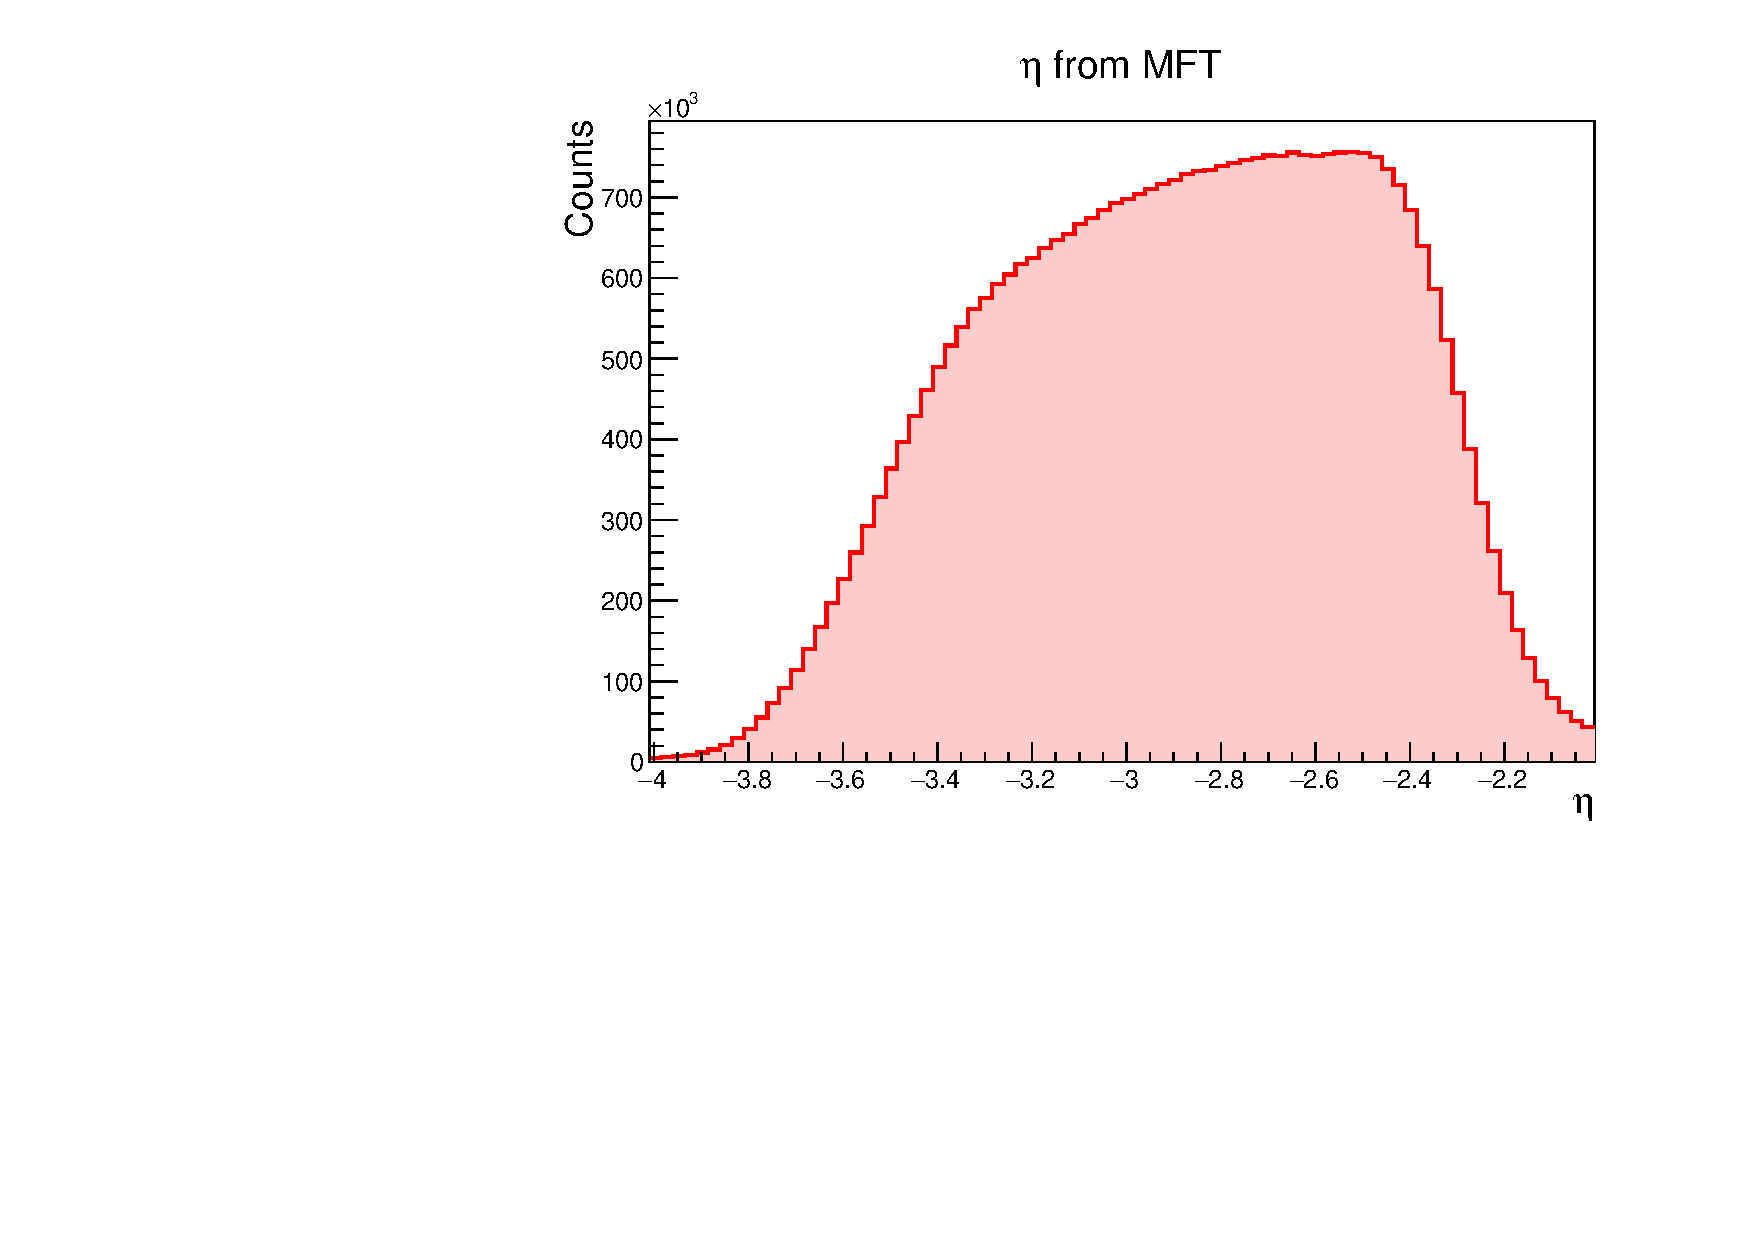
\includegraphics[width=\linewidth]{Plots/pass4_MFT/MFTeta_pass4.pdf}
        \caption{}
        \label{}
    \end{subfigure}
    \hfill
    \begin{subfigure}[t]{.49\linewidth}
        \centering
        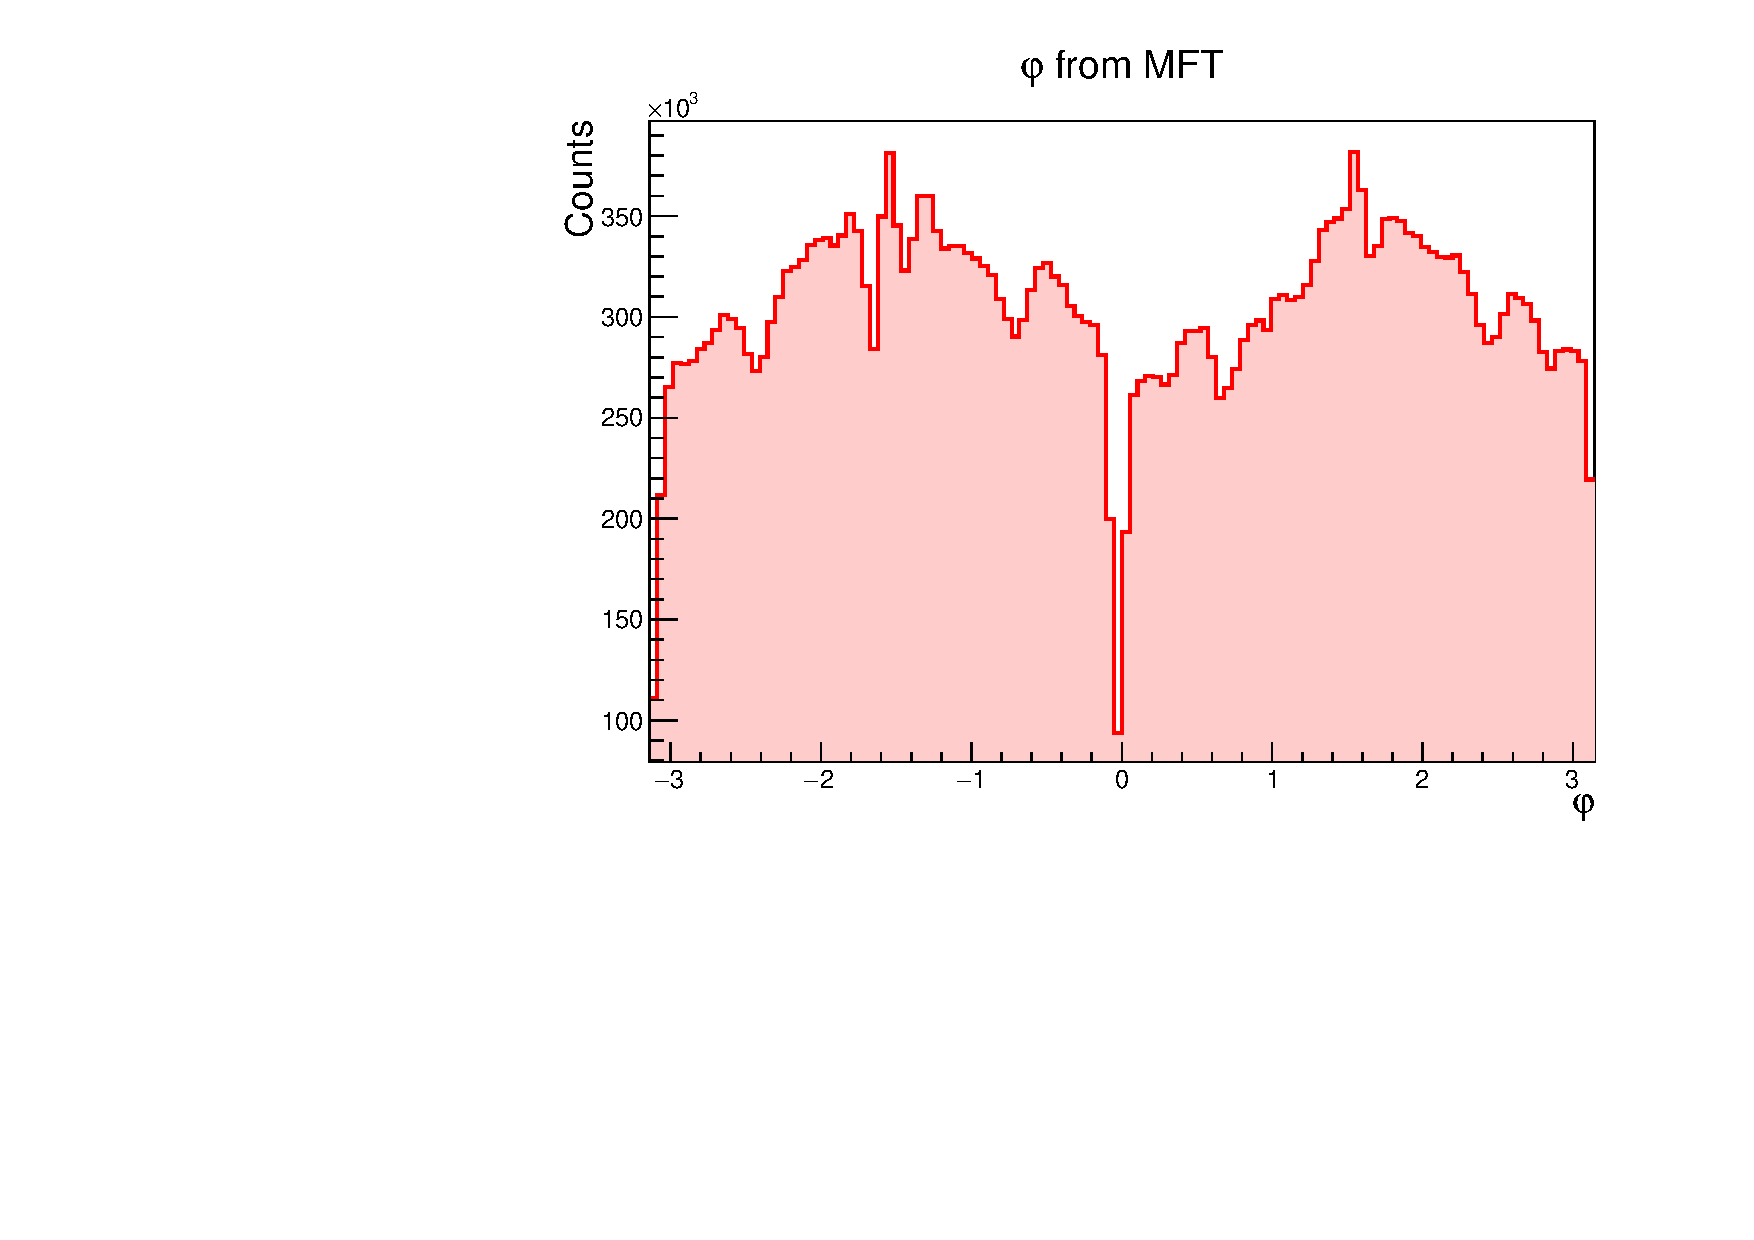
\includegraphics[width=\linewidth]{Plots/pass4_MFT/phi_pass4.pdf}
        \caption{}
        \label{}
    \end{subfigure}
    \begin{subfigure}[t]{.49\linewidth}
        \centering
        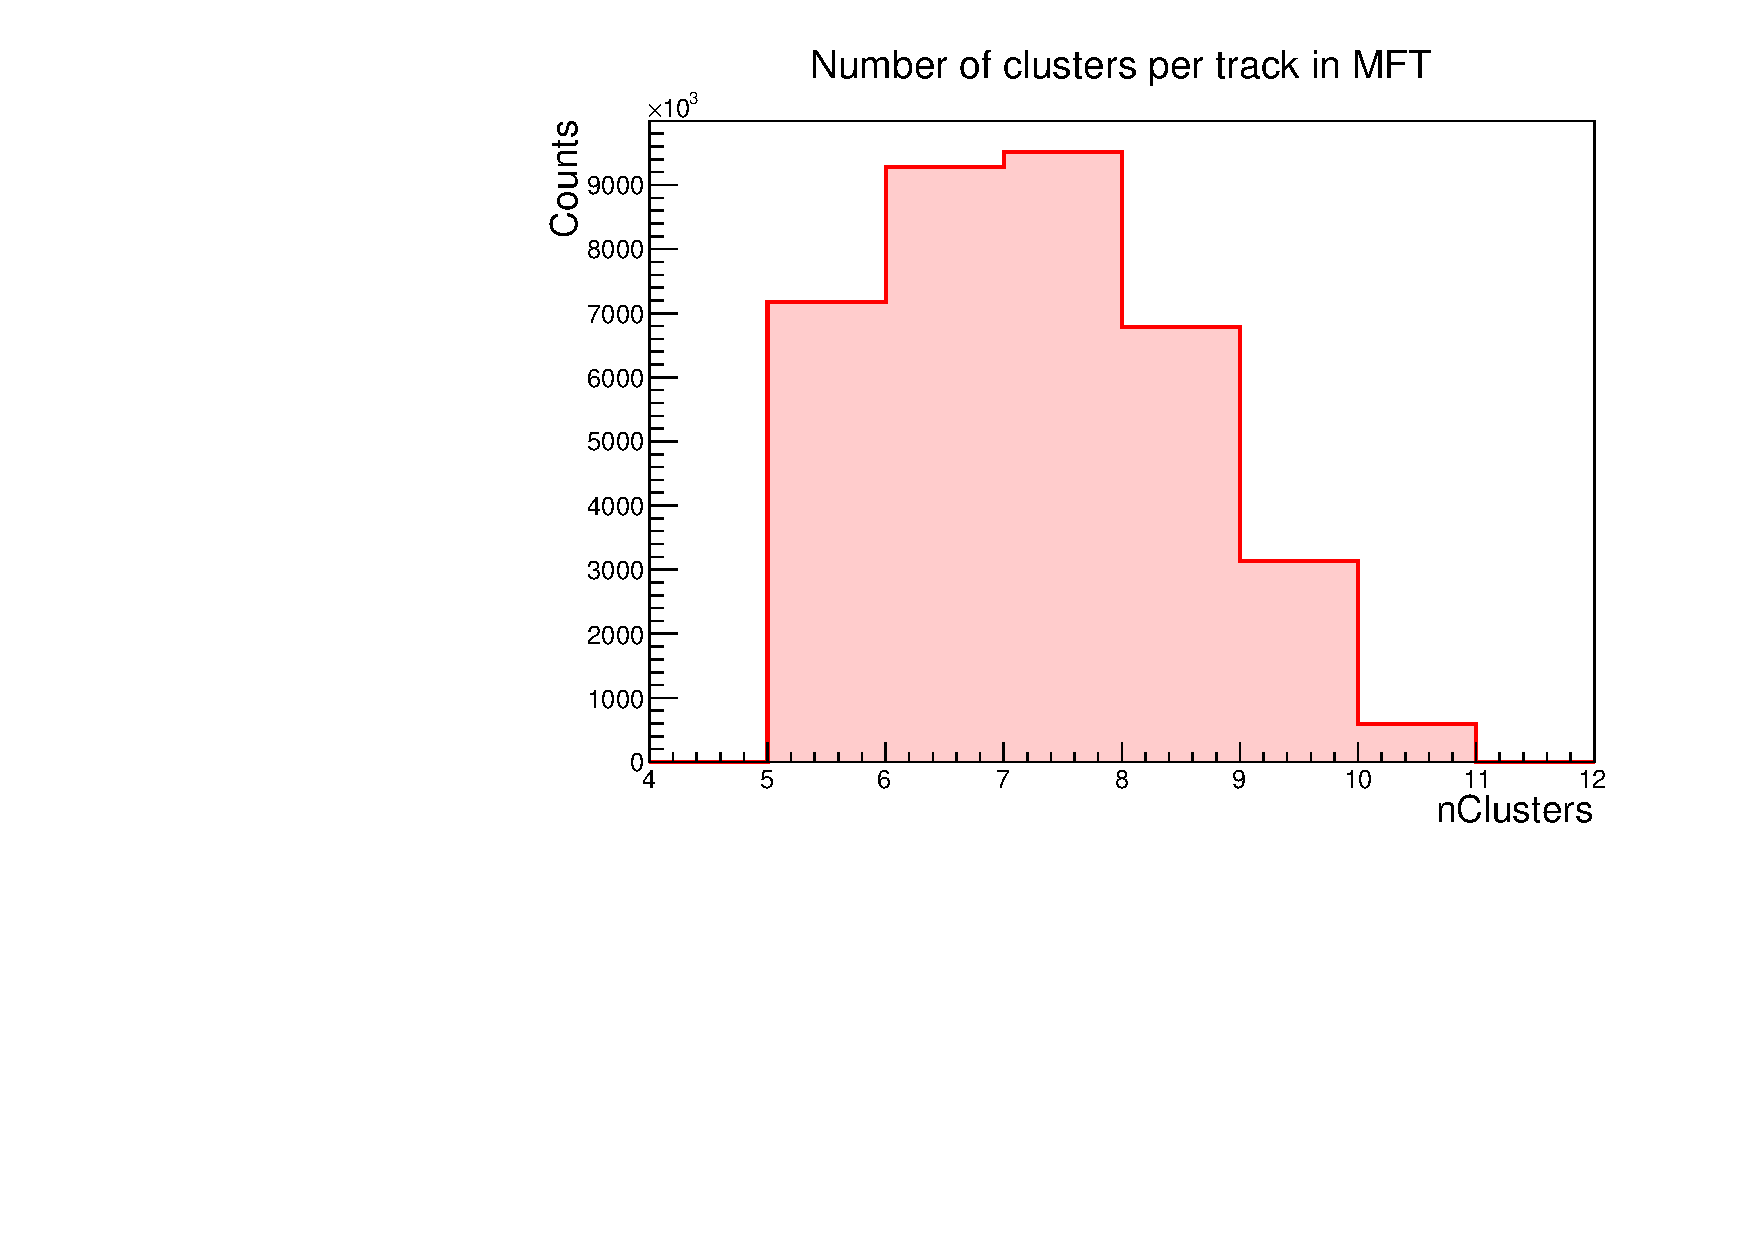
\includegraphics[width=\linewidth]{Plots/pass4_MFT/nClusters_pass4.pdf}
        \caption{}
        \label{}
    \end{subfigure}
    \hfill
    \begin{subfigure}[t]{.49\linewidth}
        \centering
        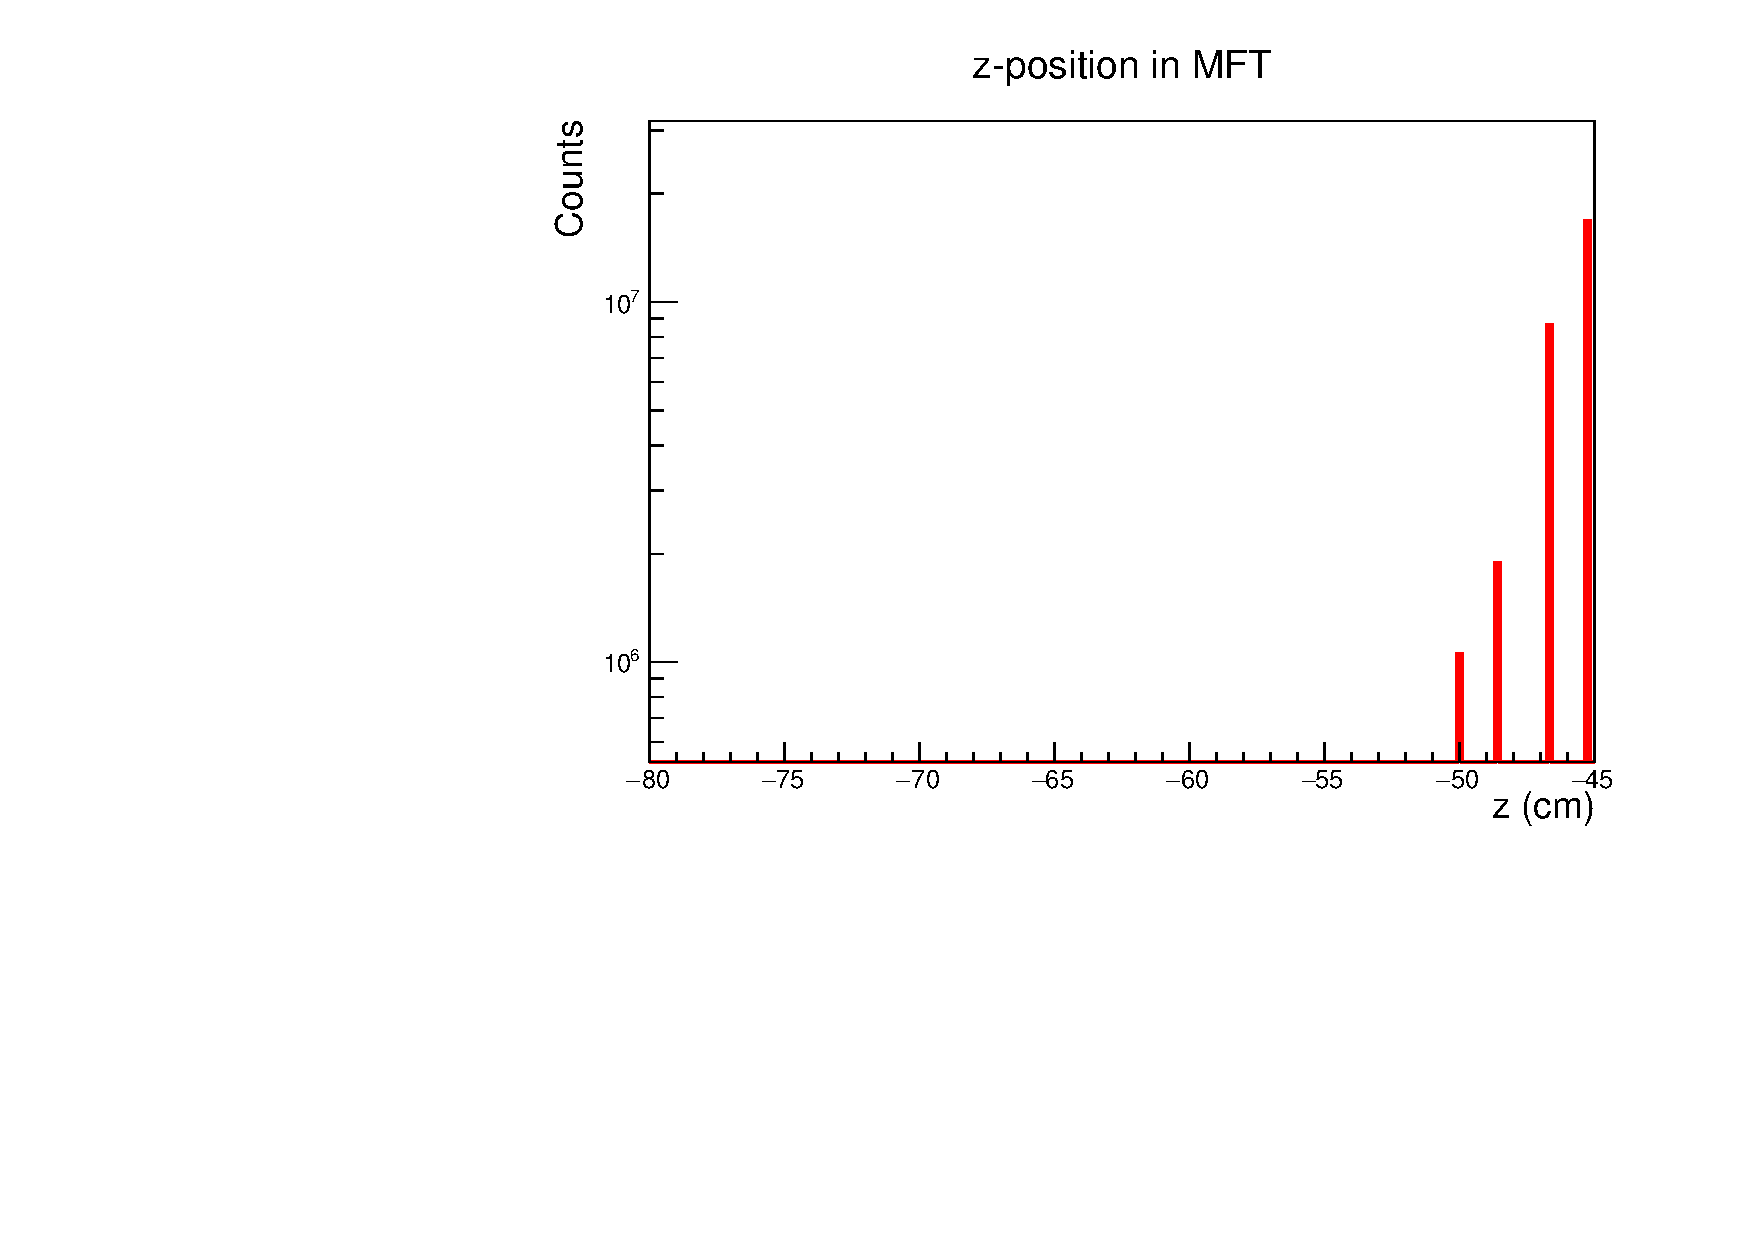
\includegraphics[width=\linewidth]{Plots/pass4_MFT/Z_MFT_pass4.pdf}
        \caption{}
        \label{}
    \end{subfigure}
\caption[Histograms of $\eta$, $\varphi$, \OldTexttt{nClusters}, and $z$ for tracks from pass 4 in the MFT]{Histograms of kinematic variables for tracks in the MFT from reconstruction pass 4. Presented here for comparison to \cref{fig:MFT_1D_pass3}. Note that other than $\eta$ there is no significant difference between these and those from pass 3. }
\label{fig:MFT_1D_pass4}
\end{figure}

\begin{figure}[h]%
    \centering
    \begin{subfigure}[t]{.49\linewidth}
        \centering
        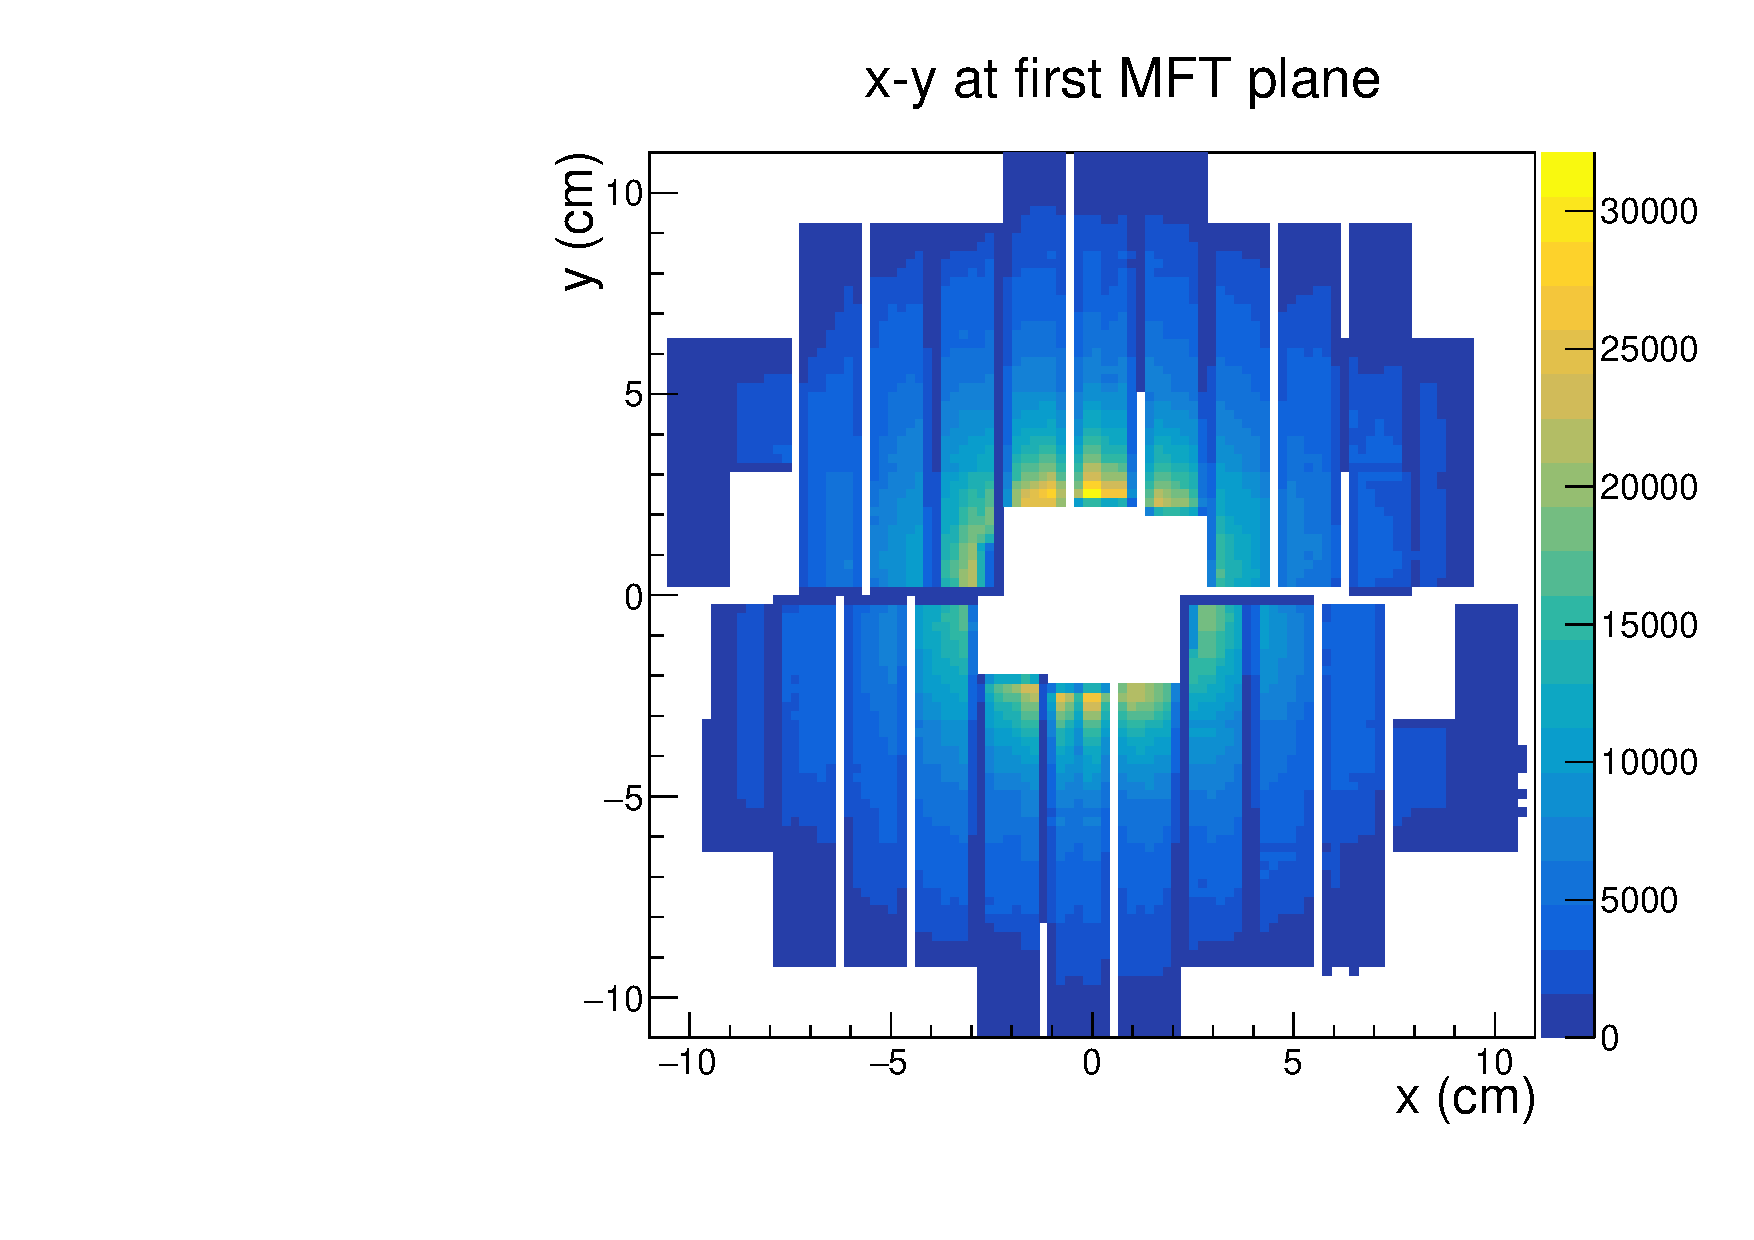
\includegraphics[width=\linewidth]{Plots/pass4_MFT/x_y_1_pass4.pdf}
        \caption{}
        \label{}
    \end{subfigure}
    \hfill
    \begin{subfigure}[t]{.49\linewidth}
        \centering
        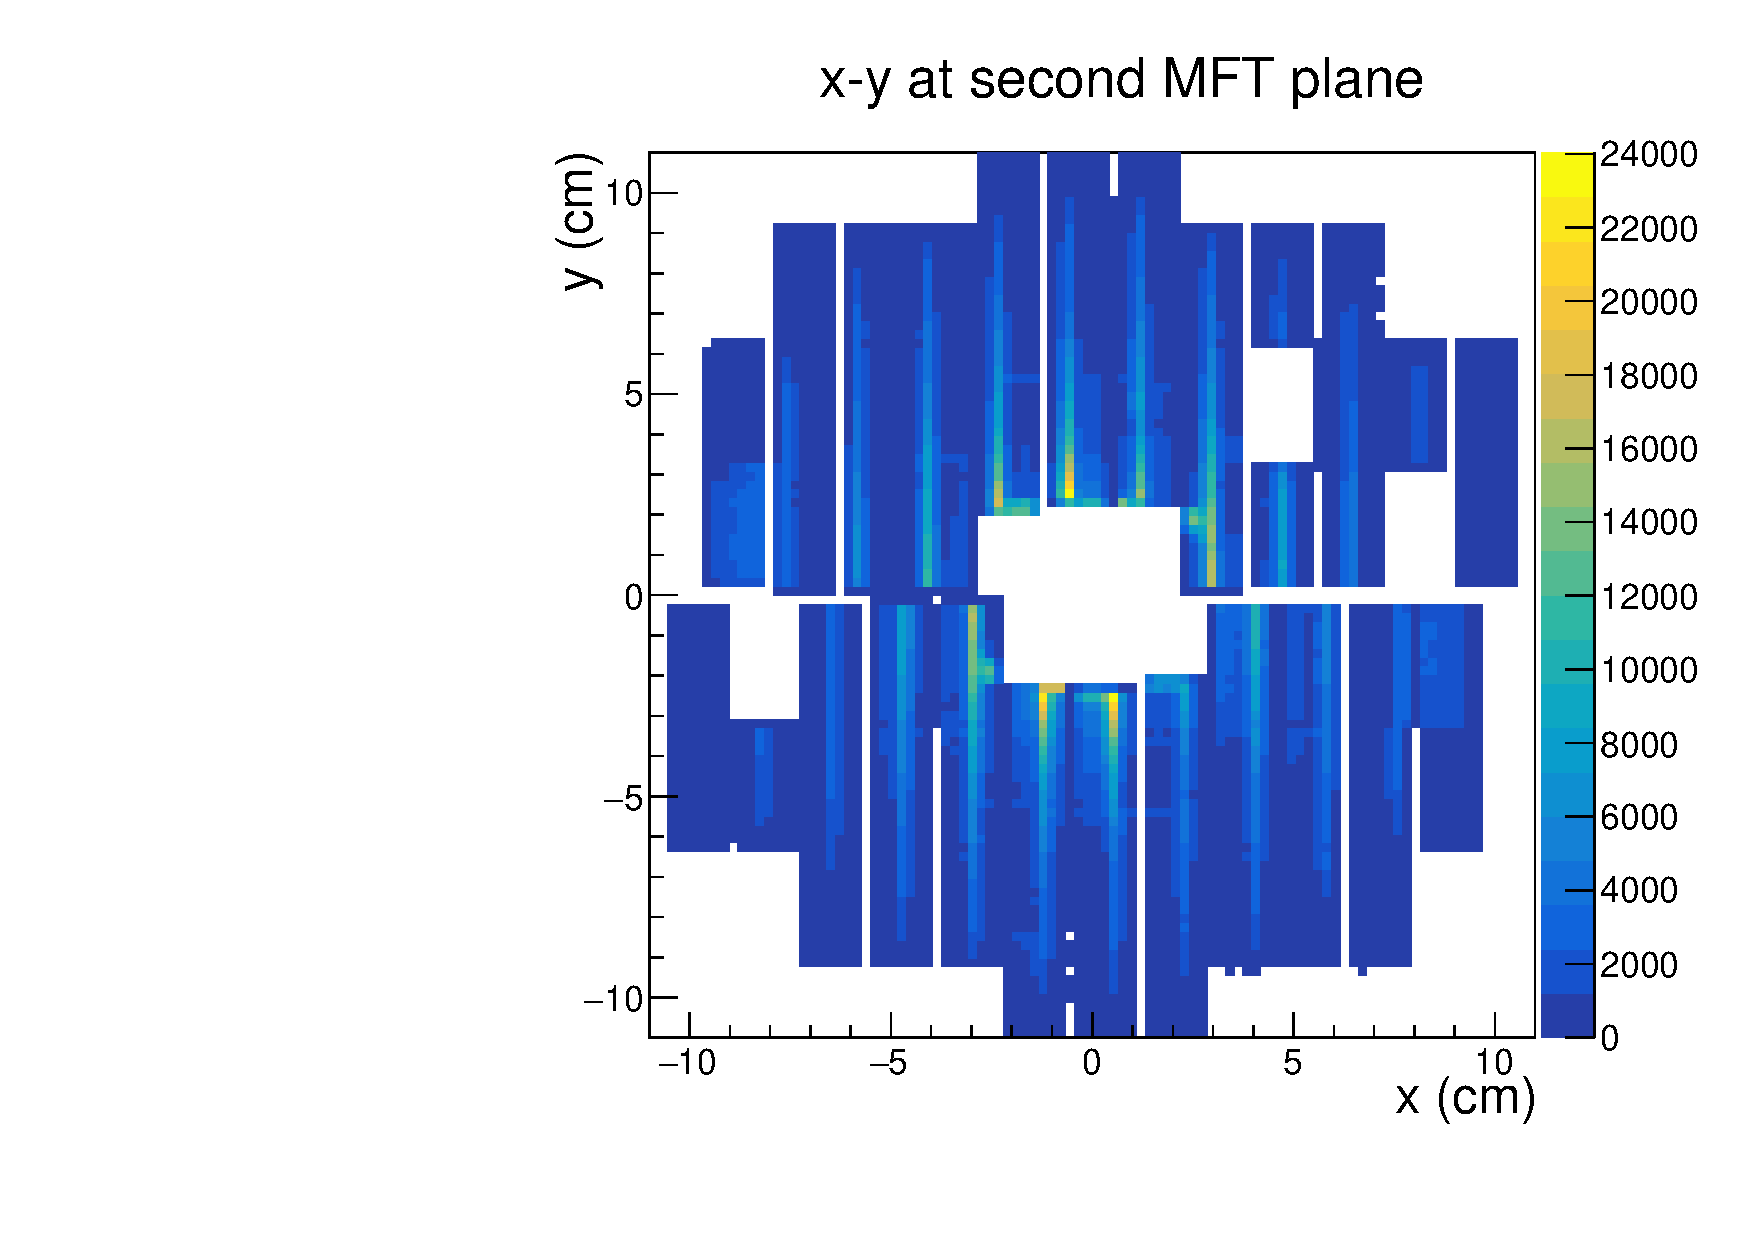
\includegraphics[width=\linewidth]{Plots/pass4_MFT/x_y_2_pass4.pdf}
        \caption{}
        \label{}
    \end{subfigure}
    \begin{subfigure}[t]{.49\linewidth}
        \centering
        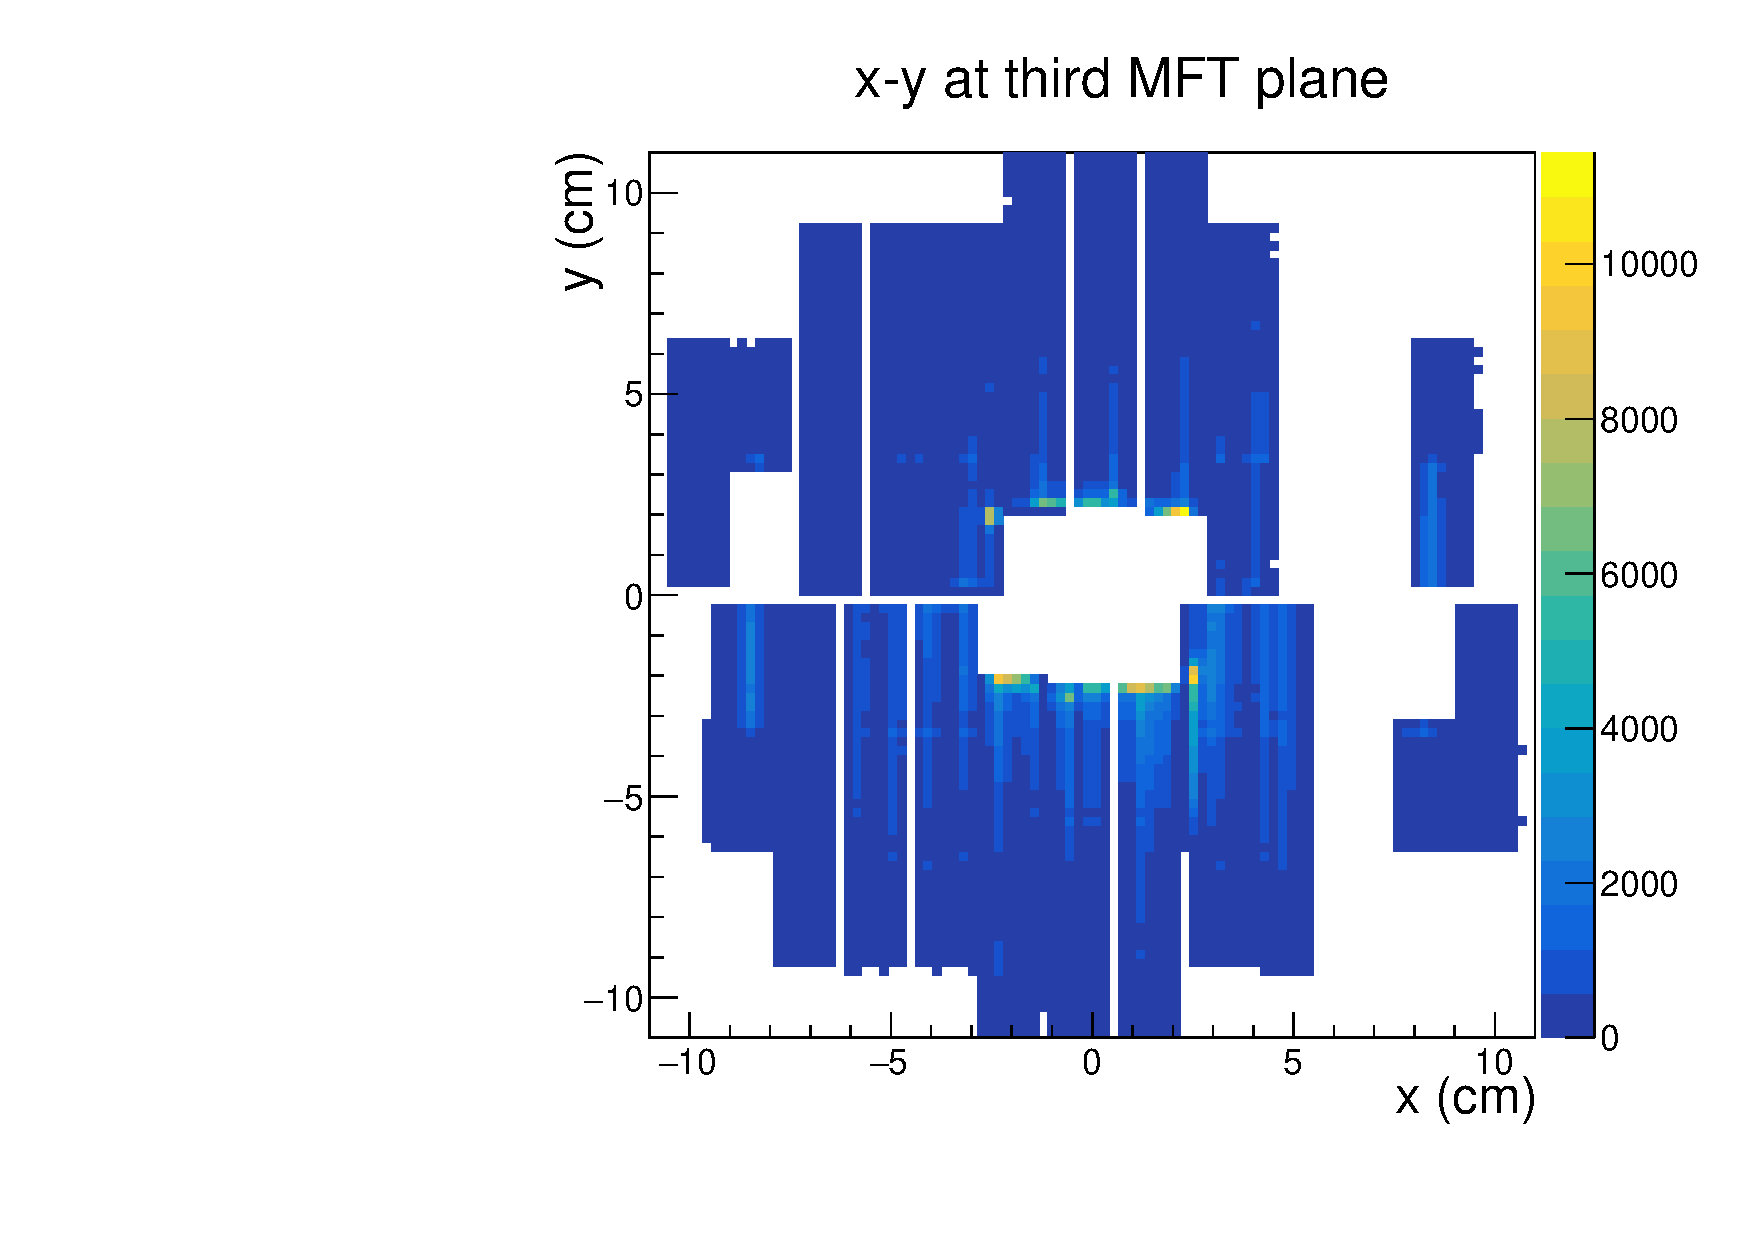
\includegraphics[width=\linewidth]{Plots/pass4_MFT/x_y_3_pass4.pdf}
        \caption{}
        \label{}
    \end{subfigure}
    \hfill
    \begin{subfigure}[t]{.49\linewidth}
        \centering
        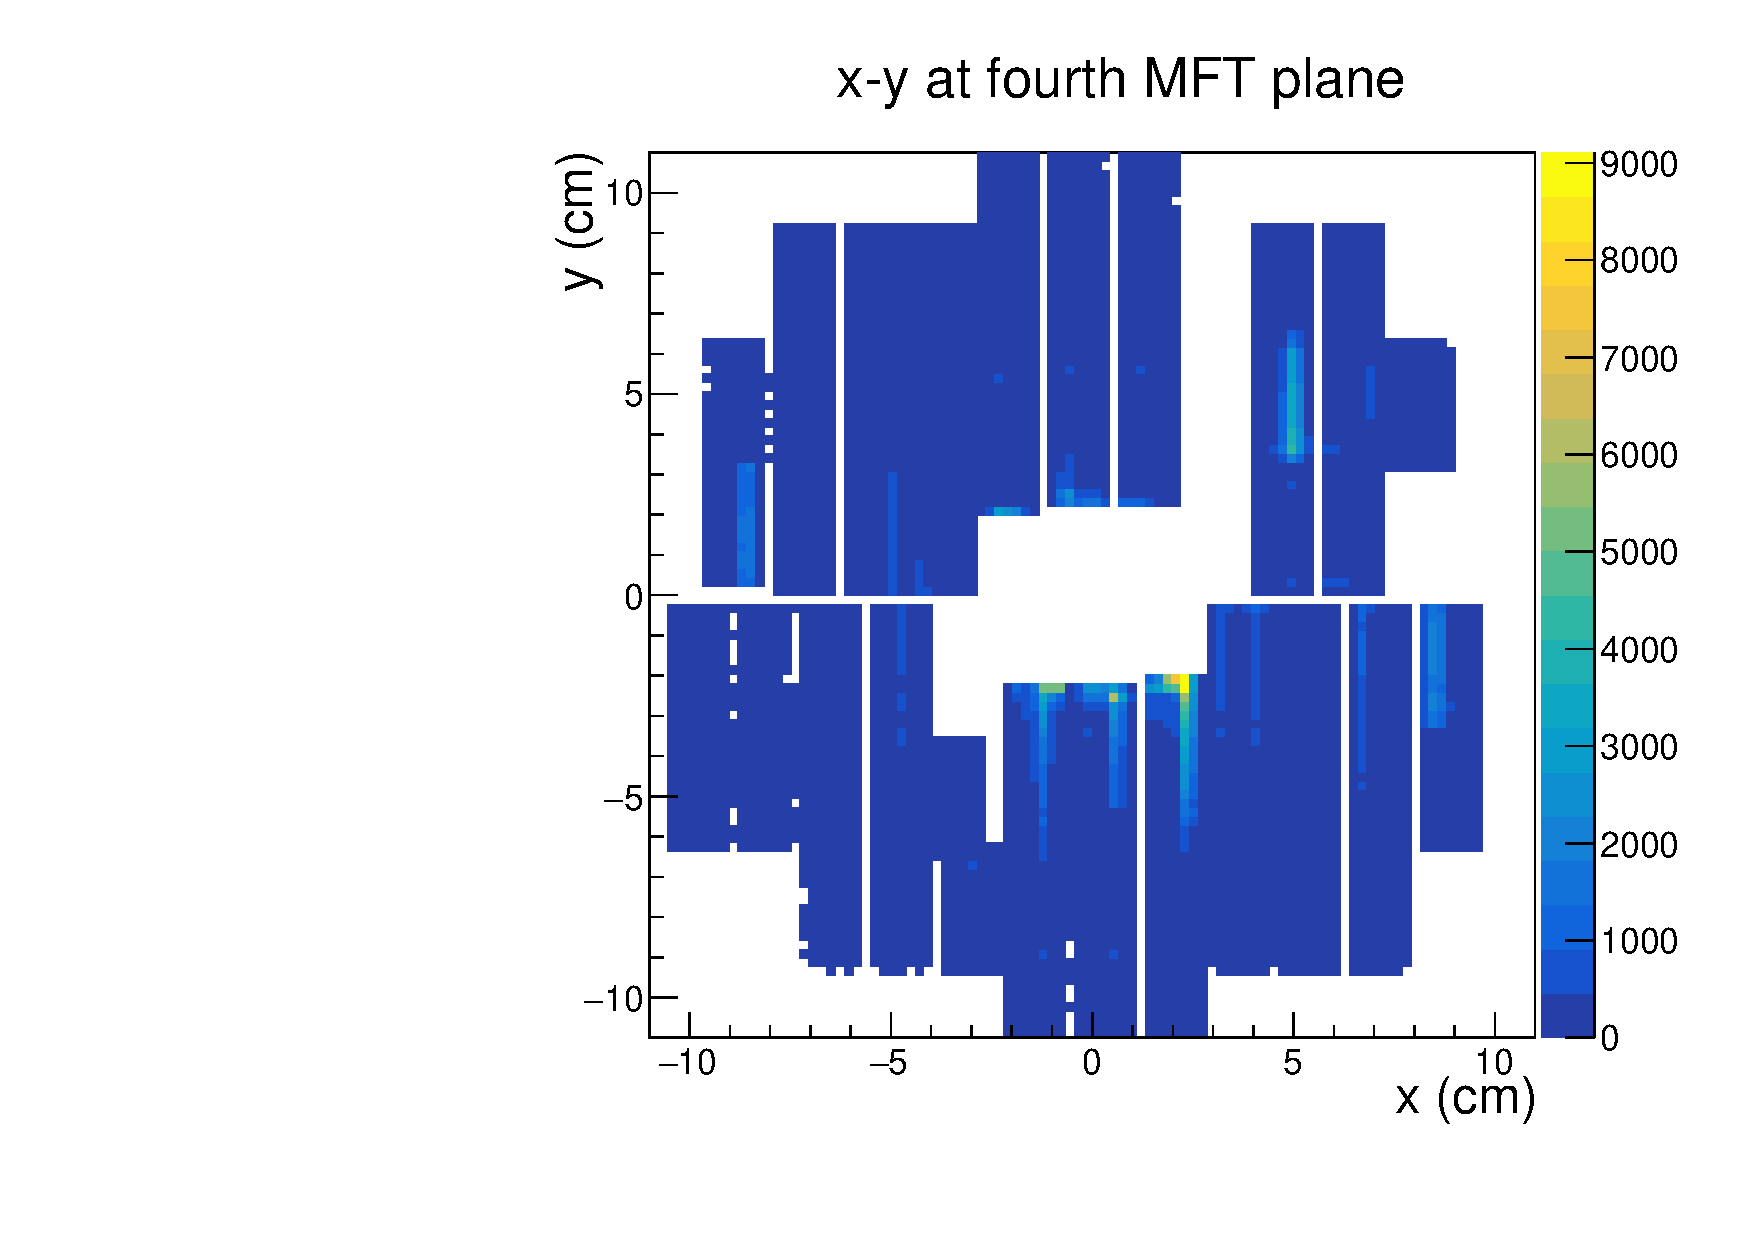
\includegraphics[width=\linewidth]{Plots/pass4_MFT/x_y_4_pass4.pdf}
        \caption{}
        \label{}
    \end{subfigure}
\caption[$x$-$y$ histograms of tracks at different planes in the MFT]{$x$-$y$ histograms for MFT tracks from reconstruction pass 4. Once again there is not much difference compared to pass 3 other than a general trend towards more uniform data. }
\label{fig:MFT_2D_pass4}
\end{figure}

\end{document}


